%&bericht

%%%%%%%%%%%%%%%%%%%%%%%%%%%%%%%%%%%%%%%%%%%%%%%%%%%%%%%%%%%%%%%%%%%%%%%%%%%%%%%
%% Descr:       Vorlage für Berichte der DHBW-Karlsruhe
%% Author:      Prof. Dr. Jürgen Vollmer, juergen.vollmer@dhbw-karlsruhe.de
%% $Id: bericht.tex,v 1.25 2020/03/13 15:07:45 vollmer Exp $
%%  -*- coding: utf-8 -*-
%%%%%%%%%%%%%%%%%%%%%%%%%%%%%%%%%%%%%%%%%%%%%%%%%%%%%%%%%%%%%%%%%%%%%%%%%%%%%%%

\documentclass[
   ngerman          % neue deutsche Rechtschreibung
  ,a4paper          % Papiergrösse
% ,twoside          % Zweiseitiger Druck (rechts/links)
% ,10pt             % Schriftgrösse
  ,12pt
% ,12pt
  ,pdftex
%  ,disable         % Todo-Markierungen auschalten
]{report}

% Bitte die Codierung Ihrer Dateien auswählen:
% \usepackage[latin1]{inputenc}    % Für UNIX mit ISO-LATIN-codierten Dateien
% \usepackage[applemac]{inputenc}  % Für Apple Mac
% \usepackage[ansinew]{inputenc}   % Für Microsoft Windows
\usepackage[utf8]{inputenc}        % UTF-8 codierte Dateien
                                   % Dieses Dokument ist unter Unix erstellt, daher
                                   % wird diese Input-Codierung benutzt.

\usepackage{bericht}
\usepackage{amsmath}
\usepackage{amssymb}
%% ACHTUNG, wenn man eine eigene Formatdatei (bericht.fmt) benutzt, werden Änderungen an bericht.sty
%% erst wirksam, wenn die Format-Datei neu erzeugt wurde!!!
%% Genauer alle Änderungen, die textuell vor der nächsten Zeile ".... endofdump...." stehen
%% werden erst wirksam, wenn die Formatdatei neu erzeugt wurde
\csname endofdump\endcsname

%%%%%%%%%%%%%%%%%%%%%%%%%%%%%%%%%%%%%%%%%%%%%%%%%%%%%%%%%%%%%%%%%%%%%%%%%%%%%%%
%% Angaben zur Arbeit
%%%%%%%%%%%%%%%%%%%%%%%%%%%%%%%%%%%%%%%%%%%%%%%%%%%%%%%%%%%%%%%%%%%%%%%%%%%%%%%

\newcommand{\Autor}{Lukas Hörnle & Marc Gökce}
\newcommand{\MatrikelNummer}{TODO}
\newcommand{\Kursbezeichnung}{TINF20B4}

\newcommand{\FirmenName}{CAS Software AG & 1&1 }
\newcommand{\FirmenStadt}{Karlsruhe}


% Falls es kein Firmenlogo gibt:
  \newcommand{\FirmenLogoDeckblatt}{}

\newcommand{\BetreuerDHBW}{Ralph Lausen}%TODO Titel von Lausen raussuchen

%%%%%%%%%%%%%%%%%%%%%%%%%%%%%%%%%%%%%%%%%%%%%%%%%%%%%%%%%%%%%%%%%%%%%%%%%%%%%%%%%%%%%

% Wird auf dem Deckblatt und in der Erklärung benutzt:
\newcommand{\Was}{Studienarbeit}
%\newcommand{\Was}{Projektarbeit}
%\newcommand{\Was}{Studienarbeit}
%\newcommand{\Was}{Bachleorarbeit}

%%%%%%%%%%%%%%%%%%%%%%%%%%%%%%%%%%%%%%%%%%%%%%%%%%%%%%%%%%%%%%%%%%%%%%%%%%%%%%%%%%%%%

\newcommand{\Titel}{
Evaluation verschiedener Bildverarbeitungsmethoden und neuronaler Netze sowie Impleymentierung eines Bildverarbeitungsverfahrens zur Segementierung und Auswertung von Füllständen in Bildern}
\newcommand{\AbgabeDatum}{22.05.2023}

\newcommand{\Dauer}{TODO raussuchen}

% \newcommand{\Abschluss}{Bachelor of Engineering}
\newcommand{\Abschluss}{Bachelor of Science}

\newcommand{\Studiengang}{Informatik}
% \newcommand{\Studiengang}{Informatik / Angewandte Informatik}

\hypersetup{%%
  pdfauthor={\Autor},
  pdftitle={\Titel},
  pdfsubject={\Was}
}

%%%%%%%%%%%%%%%%%%%%%%%%%%%%%%%%%%%%%%%%%%%%%%%%%%%%%%%%%%%%%%%%%%%%%%%%%%%%%%%

% Wenn \includeonly{..} benutzt wird, werden nur diese Kaptitel ausgegeben.
\includeonly{
  abk
 ,kapitel1
 ,kapitel2
 ,kapitel3
 ,kapitel4
 ,kapitel5
 ,kapitel6
 ,kapitel7
 ,kapitel8
 ,kapitel9
 ,kapitel10
 ,kapitel11
 ,kapitel12
 ,kapitel13
 ,kapitel14
 ,changelog
}

%%%%%%%%%%%%%%%%%%%%%%%%%%%%%%%%%%%%%%%%%%%%%%%%%%%%%%%%%%%%%%%%%%%%%%%%%%%%%%%

% Benutzt man das "biblatex"-Paket, dann muß das hier stehen:
% siehe auch die mit BIBLATEX markierten Zeilen in bericht.sty
\bibliography{bericht}

\begin{document}

%%%%%%%%%%%%%%%%%%%%%%%%%%%%%%%%%%%%%%%%%%%%%%%%%%%%%%%%%%%%%%%%%%%%%%%%%%%%%%%

\begin{titlepage}
\begin{center}
\vspace*{-2cm}
\FirmenLogoDeckblatt\hfill
\includegraphics[width=4cm]{img/dhbw-logo.png}\\[2cm]
{\Huge \Titel}\\[1cm]
{\Huge\scshape \Was}\\[1cm]
{\large für die Prüfung zum}\\[0.5cm]
{\Large \Abschluss}\\[0.5cm]
{\large des Studienganges \Studiengang}\\[0.5cm]
{\large an der}\\[0.5cm]
{\large Dualen Hochschule Baden-Württemberg Karlsruhe}\\[0.5cm]
{\large von}\\[0.5cm]
{\large\bfseries \Autor}\\[1cm]
{\large Abgabedatum \AbgabeDatum}
\vfill
\end{center}
\begin{tabular}{l@{\hspace{2cm}}l}
Bearbeitungszeitraum	         & \Dauer 			\\
Matrikelnummer	                 & \MatrikelNummer		\\
Kurs			         & \Kursbezeichnung		\\
Ausbildungsfirma	         & \FirmenName			\\%TODO hier steht aus irgendeinem Grund eine 1 
			      \empty    & \FirmenStadt			\\
Gutachter der Studienakademie	 & \BetreuerDHBW		
\end{tabular}
\end{titlepage}

%%%%%%%%%%%%%%%%%%%%%%%%%%%%%%%%%%%%%%%%%%%%%%%%%%%%%%%%%%%%%%%%%%%%%%%%%%%%%%%

%%%%%%%%%%%%%%%%%%%%%%%%%%%%%%%%%%%%%%%%%%%%%%%%%%%%%%%%%%%%%%%%%%%%%%%%%%%%%%%
%% Descr:       Vorlage für Berichte der DHBW-Karlsruhe, Erklärung
%% Author:      Prof. Dr. Jürgen Vollmer, vollmer@dhbw-karlsruhe.de
%% $Id: erklaerung.tex,v 1.11 2020/03/13 14:24:42 vollmer Exp $
%% -*- coding: utf-8 -*-
%%%%%%%%%%%%%%%%%%%%%%%%%%%%%%%%%%%%%%%%%%%%%%%%%%%%%%%%%%%%%%%%%%%%%%%%%%%%%%%

% In Bachelorarbeiten muss eine schriftliche Erklärung abgegeben werden.
% Hierin bestätigen die Studierenden, dass die Bachelorarbeit, etc.
% selbständig verfasst und sämtliche Quellen und Hilfsmittel angegeben sind. Diese Erklärung
% bildet das zweite Blatt der Arbeit. Der Text dieser Erklärung muss auf einer separaten Seite
% wie unten angegeben lauten.

\newpage
\thispagestyle{empty}
\begin{framed}
\begin{center}
\Large\bfseries Erklärung
\end{center}
\medskip
\noindent
% siehe §5(3) der \enquote{Studien- und Prüfungsordnung DHBW Technik} vom 29.\,9.\,2017 und Anhang 1.1.13
Ich versichere hiermit, dass ich meine \Was mit dem Thema:
\enquote{\Titel}
selbstständig verfasst und keine anderen als die angegebenen Quellen und Hilfsmittel benutzt habe. Ich versichere zudem, dass die eingereichte elektronische Fassung mit der gedruckten Fassung übereinstimmt.
\vspace{3cm}
\noindent
\underline{\hspace{4cm}}\hfill\underline{\hspace{6cm}}\\
Ort~~~~~Datum\hfill Unterschrift\hspace{4cm}
\end{framed}

\vfill
\emph{Sofern  vom Dualen Partner ein Sperrvermerk gewünscht wird, ist folgende Formulierungzu verwenden:}
\begin{framed}
\begin{center}
\Large\bfseries Sperrvermerk
\end{center}
\medskip
\noindent
Der Inhalt dieser Arbeit darf weder als Ganzes noch in Auszügen Personen
außerhalb des Prüfungsprozesses und des Evaluationsverfahrens zugänglich gemacht
werden, sofern keine anderslautende Genehmigung vom Dualen Partner vorliegt.
\end{framed}

%%%%%%%%%%%%%%%%%%%%%%%%%%%%%%%%%%%%%%%%%%%%%%%%%%%%%%%%%%%%%%%%%%%%%%%%%%%%%%%
\endinput
%%%%%%%%%%%%%%%%%%%%%%%%%%%%%%%%%%%%%%%%%%%%%%%%%%%%%%%%%%%%%%%%%%%%%%%%%%%%%%%


%%%%%%%%%%%%%%%%%%%%%%%%%%%%%%%%%%%%%%%%%%%%%%%%%%%%%%%%%%%%%%%%%%%%%%%%%%%%%%%

\begin{abstract}
Dieses \LaTeX-Dokument kann als Vorlage für einen Praxis- oder Projektbericht, eine Studien- oder
Bachelorarbeit dienen.

Zusammengestellt von Prof.\,Dr.\,Jürgen Vollmer \email{juergen.vollmer@dhbw-karlsruhe.de}\\
\url{https://www.karlsruhe.dhbw.de}. Die jeweils aktuellste Version dieses \LaTeX-Paketes ist immer
auf der \emph{FAQ-Seite} des Studiengangs Informatik zu finden:
\url{https://www.karlsruhe.dhbw.de/inf/studienverlauf-organisatorisches.html} $\to$ \emph{Formulare und Vorlagen}.

\centering Stand \verb+$Date: 2020/03/13 15:07:45 $+
\end{abstract}

\newpage
\tableofcontents           % Inhaltsverzeichnis hier ausgeben

% Jetzt kommt der "eigentliche" Text




\chapter{Einleitung}

\begin{center}
\begin{figure}[h]
    
\includegraphics[width=\textwidth]{img/PIA23645_PaleBlueDotRevisited_1600.jpg}
    \caption{``The Pale Blue Dot'' Feb. 14, 1990, by NASA\footnotemark.}
    \vspace{-6mm}
    \label{fig:my_label}
\end{figure}
\footnotetext{\fullcite{nasa.bluedot}}
\end{center}

''Ein Bild sagt mehr aus als tausend Worte.`` Dieses bekannte Sprichwort drückt aus, wie mächtig Bilder als Kommunikationsmittel sind. 
Bilder beinhalten Informationen, vermitteln Emotionen, erzählen Geschichten und sind ein Fenster in die Vergangenheit. 
Bilder sind in der modernen Gesellschaft omnipräsent und im Alltag digital als auch analog unentbehrlich.
Bilder unterscheiden sich je nach Aufnahme in den verschiedenen Eigenschaften ihrer Speicherung und Darstellung. 
Zwei dieser Eigenschaften sind die Größe und die Auflösung eines Bildes. 
Die Größe eines digitalen Bildes gibt an, wie viele Pixel es enthält, während die Auflösung eines Bildes angibt, wie viele Pixel pro Flächeneinheit vorhanden sind \ac{PPI}.

~

Die Größe und die Auflösung eines Bildes haben Einfluss auf seine Qualität und seinen Speicherplatzbedarf. 
Um ein Bild für einen bestimmten Zweck zu nutzen, muss es häufig in seiner Größe und oder Auflösung verändert werden. 
Der Vorgang zur Veränderung der Größe und Auflösung wird als Bildskalierung bezeichnet\footfullcite{techlib.scaling}\footfullcite{abcdef.scaling} und ist eine grundlegende Operation in der digitalen Bildverarbeitung.
Bildskalierung ist eine grundlegende Methode der Bildverarbeitung. Bildskalierung erlaubt die Änderung der Größe eines digitalen Bildes.
Eine Gute Bildskalierung misst sich an ihren Eigenschaften in den Bereichen Rechenaufwand und Qualitätsverlust. 
Besonders wichtig ist der Qualitätsverlust, wenn man Bilder größer skaliert. 
Ein geeignetes Modell um diesen Prozess zu erklären ist das übertragen einer Zeichnung von einem kleinen Papier auf eine große Leinwand. 
Wird die Zeichnung lediglich unbedacht vergrößert, wird diese unscharf und verliert an Details. 
Das Ziel einer guten Bildskalierung ist es, diesen Effekt zu verhindenr und die Zeichnung größenunabhängig scharf und detailreich darzustellen.

~

Es gibt viele verschiedene Methoden, um die Größe eines Bildes zu ändern. 
Klassische Methoden verwenden Interpolationstechniken, die neue Pixel aus den vorhandenen Pixeln berechnen. 
Diese Methoden sind schnell und stellen einen geringen Rechenaufwand in Kombination mit geringer Komplexität dar. 
Jedoch kommt es mit diesen Algorithmen oft zu Qualitätsverlusten oder der Erzeugung von Artefakten. 
Moderne Anwendungen zur Skalierung von Bildern verwenden Deep-Learning-Techniken wie Convolutional Neural Networks \ac{CNN} oder Generative Adversarial Networks \ac{GAN}, die neue Pixel aus einem trainierten Modell erzeugen. 
Diese neuen Methoden sind komplex und benötigen mehr Rechenaufwand, können allerdings die Qualität des Bildes verbessern oder kreative Effekte erstellen.

\begin{figure}[h!]
    \vspace{8mm}
    \centering
    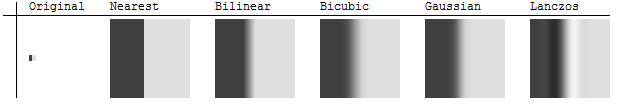
\includegraphics{img/xaR8r.png}
    \caption{Verschiedene Beispiele von upscaling Algorithmen\cite{whuber.lanczos}.}
    \label{fig:my_label}
    \vspace{4mm}
\end{figure}

Die Bildskalierung hat heute viele Anwendungen in verschiedenen Bereichen wie beispielweise Webdesign, Fotografie, Druck oder Videotechnik. 
Es gibt auch in modernen Anwendungen verschiedene Arten von Skalierungsverfahren, die sich in ihrer Funktionsweise und ihrem Ergebnis unterscheiden. 
Diese Arbeit schafft einen Überblick über klassische und moderne Skalierungsverfahren sowie deren ihre Vor- und Nachteile. 
Diese werden anhand von Beispielen inszeniert. 
Zuletzt wird basierend auf der Evaluierung der verschiedenen Verfahren eine Empfehlung für die beste Skalierungsmethode für verschiedene Bildtypen geben. 

~

In dieser Arbeit geht es darum herauszufinden, welche Methode zum Vergrößern oder Verkleinern von Bildern das beste Gleichgewicht aus Komplexität, Rechenaufwand und Ergebnissen liefert. 
Des weiteren werden die Kriterien zur Bewertung von solchen Methoden umschrieben. 
%TODO mit dem Abschnitt bin ich noch nicht happy
Dazu erklären wir zuerst die wichtigsten Konzepte der digitalen Bildverarbeitung und der Skalierung von Bildern und zeigen einige Beispiele für ihre Anwendung. Danach stellen wir die traditionellen Skalierungsmethoden vor und vergleichen ihre Stärken und Schwächen. Dann zeigen wir die neueren Skalierungsmethoden und vergleichen ihre Stärken und Schwächen. Zum Schluss bewerten wir die verschiedenen Methoden mit verschiedenen Maßstäben für die Bildqualität und geben eine Empfehlung für die beste Methode. Wir fassen unsere Ergebnisse zusammen und besprechen ihre Bedeutung und Einschränkungen.
%----------------------
\newpage




\chapter{Grundlagen der Bildverarbeitung und der Skalierung von Bildern}


\section{Einblick in die Bildverarbeitung}
Historie, Entwicklung, aktueller Stand und mögliche Entwicklungen.

\section{Skalierung von Bildern}

\subsection{Arten der Skalierungen: Interpolation und Skalierung}
    Die Interpolation und die Skalierung von Bildern oder Bildbereichen sind wichtige Konzepte der Bildverarbeitung. 
    Das Verfahren der Interpolation ermöglicht es neue Pixelwerte auf Basis vorgegebener Werte zu berechnen.
    Die Skalierung ist eine Anpassung der Bildgröße durch das Ändern der Anzahl von Pixeln oder der Auflösung.
    Im Kontext der Bildverarbeitung wird Interpolation häufig verwendet, um die Größe von Bildern zu ändern, ohne dass dabei die Anzahl der Pixel verändert wird. Dazu werden neue Pixelwerte berechnet, indem vorhandene Pixelwerte interpoliert werden. 
    Die Wahl der Interpolationsmethode hat einen großen Einfluss auf die Qualität des interpolierten Bildes. 
    In der Bildverarbeitung gibt es verschiedene Interpolationsmethoden, wie z.B. Nearest-Neighbor-Interpolation, Bilineare Interpolation oder Bikubische Interpolation.
    Skalierung hingegen verändert die Größe eines Bildes, indem die Anzahl der Pixel oder die Auflösung verändert wird. 
    Im Gegensatz zur Interpolation wird die Anzahl der Pixel bei der Skalierung verändert, um das Bild kleiner oder größer zu machen. 
    Auch hier hat die Wahl der Skalierungsmethode einen großen Einfluss auf die Qualität des resultierenden Bildes.

\subsection{Bildformate}
    Bilder können allgemein als zweidimensionaler Array dargestellt werden.
    Historisch gesehen gab es jedoch viele unterschiedliche Formate für Bilder. 
    Zunächst erschufen unterschiedliche Softwareentwickler im Bereich der Bildverarbeitung häufig ihre eigenen Formate.\footfullcite{burger2009digitale}
    Einheitliche Standards, wie sie heute im Einsatz sind, etablierten sich erst später.
    Ein Vorreiter der modernen Bildformate ist das "Portable Network Graphics Format"\footfullcite{boutellpng}, das 1985 in den USA vorgestellt wurde. 
    Moderne Dateiformate zur Speicherung von Bildern werden anhand der Art des Bildes sowie der Kriterien Speicherbedarf und Kompression, Kompatibilität und ihrem Anwendungsbereich bewertet. 
    \footfullcite{burger2009digitale}
    
    \subsubsection{Portable Network Graphics Format}
        Portable Network Graphics Format \ac{PNG} setzt einen besonderen Fokus auf eine geringe Komplexität und eine einfache Implementierung des Standards. 
        Der Standard kann frei von jedem genutzt werden.
        Des weiteren profitiert das Format von verlustfreier Kompression. \footfullcite{boutell1997png}
        PNG unterstützt Vollfarbbilder, Grauwertbilder sowie Indexbilder. \footfullcite{burger2015digitale}
        Der PNG-Algorithmus komprimiert Bilder, indem er mehrere Techniken, einschließlich Filterung und Huffman-Codierung anwendet. 
        Zunächst wird das Bild in Blöcke von 16 x 16 Pixeln aufgeteilt und dann wird auf jedem Block ein Filter angewendet, um Redundanzen zu entfernen. 
        Anschließend wird das Ergebnis der Filterung Huffman-codiert, um eine effiziente Darstellung der Daten zu erreichen.
        Characteristisch für PNG-Dateien ist auch die Möglichkeit, transparente Flächen einzubauen. 
        Der Standard verwendet eine spezielle Methode, um Transparenz darzustellen. 
        Diese wird als Alpha-Kanal bezeichnet und ermöglicht es, transparente sowie halbtransparente Bilder zu erstellen.
        Die kompekte Komprimmierung des PNG-Formats hat dafür gesorgt, dass der Standard im Internet eine hohe Beliebtheit genießt. 
        \footfullcite{^w3c_png}
    
    \subsubsection{JPG-Format}
        \ac{JPG}
        %TODO und Acronym für JPG
        Hier noch text bittö.
        
    
    \subsubsection{Scalable Vector Graphics}
        \begin{quote}
            The main idea motivating \ac{SVG} was simple: to create a generic document-oriented solution  for graphics that can be adapted to modern media
            \grqq{}~\footfullcite{book:729077}
        \end{quote}
        %Evaluation und Implementierung eines Bildverarbeitungsverfahrens zur Füllstandsmessung
        Scalable Vector Graphics (SVG) steht für ein Format, das Vektorgrafiken basierend auf \ac{XML} darstellt.
        Im Gegensatz zu Rastergrafiken, wie z.B. PNG, die aus Pixeln bestehen und bei Vergrößerung an Schärfe verlieren, sind Vektorgrafiken vektorbasiert und behalten ihre Qualität bei beliebiger Skalierung. 
        Der Standard ermöglicht eine besonders effiziente Speicherung von Bildern.
        SVG ist außerdem ein offenes Format und unterstützt Interaktivität, Animation und Skripting.\footfullcite{quint2003scalable} 
        Da SVG auf XML basiert, kann es auch mit anderen Webtechnologien wie HTML, \ac{CSS} und JavaScript integriert werden.\footfullcite{mdn_svg} 
        
    \subsubsection{Weitere Standards}
        %TODO MEHR TEXT!!!! 
        \begin{description}
            \item[\ac{GIF}]~\\
                Ein Format für animierte Rastergrafiken mit einer begrenzten Farbpalette von 256 Farben. 
                Es verwendet eine verlustfreie Kompression, die aber nicht sehr effizient ist. 
                Es ist geeignet für einfache Animationen und Grafiken mit wenigen Farben.
            \item[\ac{TIFF}]~\\
                Ein Format für hochauflösende Rastergrafiken ohne Kompression oder mit verlustfreier Kompression.
                Es wird oft im Druckbereich verwendet, da es viele Optionen für Farbmanagement und Metadaten bietet.
                Es ist aber nicht sehr kompatibel mit Webbrowsern \\
            \item[\ac{PSD}]~\\
                Ein Format für Photoshop-Dokumente, das alle Ebenen, Masken, Effekte und andere Informationen speichert.
                Es ermöglicht eine umfangreiche Bearbeitung von Rastergrafiken, ist aber nur mit Photoshop kompatibel.\\
            \item[\ac{BMP}]~\\
                Ein Format für unkomprimierte Rastergrafiken mit hoher Qualität.
                Es wird selten verwendet, da es sehr große Dateien erzeugt und keine Transparenz oder andere Funktionen unterstützt. \\
            \item[\ac{EPS}]~\\
                Ein Format für vektorbasierte Grafiken, das Kurven, Texte und andere Elemente speichert.
                Es kann skaliert werden ohne Qualitätsverlust und wird oft im Druckbereich verwendet.
                Es ist aber nicht sehr kompatibel mit Webbrowsern oder anderen Programmen. \\
        \end{description}
        Weiterhin gibt es unzählige Standards um Grafiken darzustellen. Diese übersteigen jedoch den Umfang dieser Arbeit.
        \footfullcite{prepressure_file_formats}\footfullcite{ionos_file_formats}\footfullcite{rabbani2002overview}\footfullcite{marcellin2000overview}\footfullcite{britannica_jpeg}\footfullcite{elsevier_artwork}
\subsection{Wichtige Aspekte der Skalierung}
    \subsubsection{Segmentierung}
    
        Die Segmentierung von Bildern ist ein wichtiges Verfahren der Bildverarbeitung, da es ermöglicht, ein Bild in sinnvolle Regionen zu unterteilen. 
        Hierbei können verschiedene Verfahren, wie Schwellenwert- oder Clustering-Methoden eingesetzt werden. 
        Die Genauigkeit der Segmentierung hängt dabei maßgeblich von der Komplexität des Bildes und der gewählten Methode ab.
        Eine erfolgreiche Segmentierung kann für viele Anwendungen von Nutzen sein.
        Die automatischen Erkennung von Gesichtern oder die Identifizierung von Verkehrszeichen auf Straßenbildern sind die populärsten Beispiele.
        Jedoch ist es oft schwer genaue Grenzen zwischen Objekten in Bildern mit komplexen Strukturen zu erkennen.
    
    \subsubsection{Klassifizierung}
    
        Die Klassifizierung von Bildinhalten ist ein weiterer wichtiger Aspekt der Bildverarbeitung.
        Hierbei werden Bilder in automatisch bestimmte Kategorien eingeteilt. 
        Beispielanwendungen inkludieren das Erkennen von Tierarten auf Naturfotos oder das Identifizieren von Gesichtern auf Fotos. 
        Hierfür können verschiedene Techniken verwendet werden. Beispiele sind Deep Learning oder Entscheidungsbaum-Algorithmen.
        Eine erfolgreiche Klassifizierung kann für viele Anwendungen genutzt werden, wie zum Beispiel zur Automatisierung von Aufgaben oder im maschinellen Lernen. 
        Die Geneauigkeit einer Klassifizierung wird von Faktoren, wie zum Beispiel von der Qualität der Trainingsdaten oder der Komplexität der verwendeten Klassifikationsmethode beeinflusst.
    
    \subsubsection{Objekterkennung und -verfolgung}
    
        Die Objekterkennung und -verfolgung ist ein wichtiger Aspekt der Bildverarbeitung, der oft in Anwendungen wie der Überwachung und Robotik genutzt wird. 
        Hier geht es darum, Objekte in Bildern oder Videos zu erkennen und ihre Bewegungen zu verfolgen. 
        Es können verschiedene Techniken eingesetzt werden, wie zum Beispiel Hintergrundsubtraktion oder optische Flussberechnung.
        Eine erfolgreiche Objekterkennung und -verfolgung kann für viele Anwendungen genutzt werden, wie zum Beispiel in der Videoüberwachung oder bei der Steuerung von autonomen Fahrzeugen. 
        Allerdings gibt es auch Herausforderungen bei der Objekterkennung und -verfolgung, wie zum Beispiel die Bewältigung von Hintergrundrauschen oder die Verfolgung von Objekten bei hoher Geschwindigkeit.
    
    \subsubsection{3D-Bildverarbeitung}
        In der 3D-Bildverarbeitung werden dreidimensionale Bilder und Modelle analysiert und verarbeitet.
        Die Anwendungsfelder dieser Technologien reichen von medizinischen Umgebungen bis hin zur industriellen Fertigung.
        In bildgebenden medizinischen verfahren werden 3D-Bilder für die Diagnose von Krankheiten und Verletzungen verwendet. 
        In der industriellen Fertigung werden 3D-Modelle für die Qualitätssicherung und die Fehlererkennung verwendet.
    
    \subsubsection{Bildkompression}
        Da Bilder in der Regel große Datenmengen erzeugen, die für die Übertragung und Speicherung unpraktisch sind, benötigt es oft eine Bildkompression. 
        Durch Kompressionstechniken wie z.B. die JPEG-Kompression kann die Größe von Bildern erheblich reduziert werden ohne dabei große QUalitätsverluste zu erleiden.
    
\section{Echtzeitverarbeitung von Bildern}

    Die Echtzeitverarbeitung von Bildern stellt eine Herausforderung in der Bildverarbeitung dar, da eine sehr schnelle Verarbeitung notwendig ist, um zeitkritische Anwendungen wie z.B. autonomes Fahren oder Augmented Reality zu realisieren.
    Bei diesen Aufgaben müssen Bilder in Echtzeit erfasst, verarbeitet und angezeigt werden, um eine reibungslose Funktionalität zu gewährleisten.
    Die Echtzeitverarbeitung von Bildern erfordert in der Regel eine hohe Rechenleistung, um die Daten schnell genug zu verarbeiten.
    Hierbei kommen spezielle Algorithmen zum Einsatz, die für eine effiziente Verarbeitung sorgen.
    Eine weitere Herausforderung bei der Echtzeitverarbeitung von Bildern ist die Echtzeit-Kommunikation zwischen den verschiedenen Komponenten des Systems. 
    Hierbei müssen Daten schnell und zuverlässig ausgetauscht werden, um Verzögerungen zu vermeiden. 
    Hierfür kommen oft spezielle Systeme zum Einsatz, die für eine schnelle Übertragung und parallele Verarbeitung von Daten optimiert sind.
    \footfullcite{oehlrich1992transputersystem}
\section{Anwendungen von Skalierungsmethoden}
    % help
    Die Anwendung von Skalierungsmethoden bietet eine Vielzahl ungewöhnlicher, aber äußerst nützlicher Anwendungen in verschiedenen Sektoren.
    In der Landwirtschaft können diese Methoden dazu beitragen, die Gesundheit von Pflanzen zu überwachen und den Einsatz von Pestiziden zu optimieren.
    Durch die Analyse von Pflanzenbildern können frühzeitig Krankheiten erkannt und gezielte Maßnahmen ergriffen werden, um Ernteausfälle zu minimieren.
    In der Archäologie ermöglichen Skalierungsmethoden die digitale Rekonstruktion verwitterter oder beschädigter Artefakte.
    Dies eröffnet Forschern neue Einblicke in die Geschichte vergangener Zivilisationen und ermöglicht die Erstellung interaktiver virtueller Museen.
    In der Modeindustrie ermöglichen Skalierungsmethoden das virtuelle Anprobieren von Kleidung, was den Kunden die Möglichkeit gibt, Passform und Aussehen der Kleidungsstücke im Voraus zu überprüfen und das Online-Shopping-Erlebnis zu verbessern.
    Durch die Integration von Bildverarbeitung und Augmented Reality entsteht eine innovative und interaktive Shopping-Erfahrung.
    Insgesamt bieten Skalierungsmethoden in diesen verschiedenen Sektoren ungewöhnliche Anwendungen, die zu Effizienzsteigerungen, Erkenntnisgewinnen und verbesserten Kundenerfahrungen führen.

\chapter{Klassische Skalierungsmethoden}

    \section{Pixel-Verdopplung}

        \begin{figure}[h]
            \centering
            
\includegraphics[width=0.6\textwidth]{img/so_sieht_pixel_verdopplung_aus.jpg}
            \caption{Beispielhafte Darstellung einer Skalierung durch PixelVerdopplung}
            \label{fig:beispielhafte_darstellung_einer_skalierung_durch_pixelverdopplung}
        \end{figure}

        Die Pixel-Verdopplung vergrößert das Bild, indem jeder Pixel dupliziert wird.
        Diese Methode kann schnell und einfach umgesetzt werden, indem jeder Pixelwert einfach auf den Nachbarpixel übertragen wird.
        Wenn Bilder mit dieser Methode stark vergrößert werden, ergeben sich oft pixelige und unscharfe Ausgaben, da die Details nicht wirklich vorhanden sind, sondern nur durch die Duplizierung von Pixeln aufgefüllt werden. 
        Aus diesem Grund wird Pixel-Verdopplung oft als eine minderwertige Skalierungsmethode betrachtet und findet in professionellen Anwendungen selten Gebrauch.~\footfullcite{WANG1983363}


    \newpage
    Eine beispielhafte Implementierung in Python sieht folgendermaßen aus:
    
    \begin{lstlisting}[caption={Python-Klasse zur Pixelverdopplung und Bildmanipulation: Implementierung des Algorithmus mit der Pillow-Bibliothek und Erklärung des Codes von PixelVerdopplung: \url{https://github.com/studienarbeit-cnn-dhbwka-2022/Code/blob/main/backend/skalierungsmethoden/pixel_verdopplung.py}.}]
    class PixelVerdopplung(Image):
        def __init__(self, path):
            extend = "p2"
            super().__init__(path, extend)
        
        def manipulate(self, new_size):
            super().manipulate(new_size)
        
            for y in range(self.new_height):
                for x in range(self.new_width):
                    x_old = int(x / (self.new_width / self.width))
                    y_old = int(y / (self.new_height / self.height))
        
                    # Check that x_old and y_old are within bounds of original image
                    if x_old >= self.width:
                        x_old = self.width - 1
                    if y_old >= self.height:
                        y_old = self.height - 1
        
                    old_pixel = self.img.getpixel((x_old, y_old))
                    self.newImg.putpixel((x, y), old_pixel)
        
            return self.save()
    \end{lstlisting}
        
        Die vorliegende Implementierung in Python beschreibt die Realisierung der Pixelverdopplungsklasse, welche in der Lage ist, ein größeres Bild zu erzeugen, indem die leeren Pixel mit demselben Pixelwert wie der nächste Nachbarpixel befüllt werden.
        Der Code ist darauf ausgelegt, eine einfache Möglichkeit bereitzustellen, um ein Bild auf eine höhere Auflösung zu skalieren, wodurch fehlende Details ausgeglichen werden können.
        Dabei wird eine lineare Interpolation auf der Basis der Nachbarpixel durchgeführt, um das neue Bild zu generieren.
        Die Klasse "PixelVerdopplung" erbt von der Klasse "Image" und besitzt einen Konstruktor, der den Pfad zum Bild und die Erweiterung "p2" als Argumente erhält. 
        Die Methode "manipulate" ist dafür zuständig, das Bild auf die gewünschte Größe zu skalieren und zu manipulieren.
        Innerhalb der Methode werden Schleifen durchlaufen, um jeden neuen Pixel im manipulierten Bild zu generieren. 
        Die Koordinaten des jeweiligen alten Pixels werden durch Division der neuen Koordinaten durch die Skalierungsfaktoren berechnet und auf den nächstgelegenen Integer gerundet.
        Um sicherzustellen, dass die berechneten Koordinaten innerhalb der Grenzen des ursprünglichen Bildes liegen, werden sie in einem nächsten Schritt auf den maximalen Index des Bildes zurückgesetzt, falls sie außerhalb liegen sollten. 
        Anschließend wird der Pixelwert des entsprechenden alten Pixels abgerufen und als neuer Pixel an der berechneten Stelle im neuen Bild platziert.
        Die Implementierung dieses Algorithmus stellt eine einfache Möglichkeit dar, um ein Bild auf eine höhere Auflösung zu skalieren, wodurch ein besseres visuelles Ergebnis erzielt werden kann. 
        Dabei ist darauf zu achten, dass die lineare Interpolation eine höhere Laufzeit und Speicheranforderungen aufweist als andere Interpolationsmethoden.
        
    \section{Nearest-Neighbor-Interpolation}
        Die Nearest-Neighbor-Interpolation ist eine weitere Methode zur Skalierung von Bildern. 
        Es wird für jedes Pixel im Ausgabebild der am nächsten liegende Pixel im Eingabebild ausgewählt und der Farbwert des ausgewählten Pixels wird als Farbwert des entsprechenden Pixels im Ausgabebild verwendet.
        Die Verwendung von Nearest-Neighbor-Interpolation ist einfach und schnell zu implementieren. 
        Aufgrund ihrer geringen Komplexität ist sie daher sehr beliebt. 
        Die Methode eignet sich besonders gut für die Vergrößerung von Bildern mit großen, einheitlichen Bereichen oder harten Kanten. 
        

        \begin{acronym}
          \acro{NNI}{Nearest Neighbor Interpolation}
        \end{acronym}
        \begin{lstlisting}
        import numpy as np
        import cv2
        
        def nearest_neighbor_interpolation(image, scale_factor):
            new_size = (int(image.shape[1] * scale_factor), int(image.shape[0] * scale_factor))
            
            scaled_image = np.zeros(new_size + (image.shape[2],), dtype=np.uint8)
            for i in range(new_size[0]):
                for j in range(new_size[1]):
                    x = int(i / scale_factor)
                    y = int(j / scale_factor)
                    scaled_image[j, i] = image[y, x]
            
            return scaled_image
        
        
        image = cv2.imread('example_image.jpg')
        scaled_image = nearest_neighbor_interpolation(image, 2)
        cv2.imshow(image)
        cv2.imshow(scaled_image)
        \end{lstlisting}\footfullcite{jiang2015quantum}
        %TODO @Marc kannst du mir ne Schöne Grafik machen, wo du diesen Code kurz über unser Beispielbild laufen lässt und wir so nen rechts/links Vergleich haben?

        Bei der Verkleinerung von Bildern erleiden diese jedoch oft einen Qualitätsverlust.
        Hier kommt es zu Unschärfe und Blockbildung.
        Dieser Effekt verstärkt sich, wenn das Verhältniss zwischen Quellbild und Audgabebild kein Vielfaches ist.

    \section{Bilineare Interpolation}
    
    % Interpolation cool weil, schnell und ergebniss recht schön.

    % Bilinear ist well aus 2 pixel linear interpoliert wird. (Bild farbig)
    % Die Distanz wir linear berechnet aus den 4 nachbar pixel (Graph 2 punkte)
    % wird fast überall genutzt (citation und quelle angeben)
    
    % Vorteile: Schnell und kompilizert zu programmieren, sieht nicht beschissen aus und kann immer angewendet werden
    % Nachteile: Sieht nicht perfekt aus (Siehe Bicubic oder lanzeros) - ist bei extremen skalierungen nicht super

        Die bilineare Interpolation ist eine weit verbreitete Methode zur Skalierung von Bildern.
        Sie basiert auf dem Konzept der linearen Interpolation und wird häufig in Grafikanwendungen und Bildverarbeitungsalgorithmen eingesetzt.
        Bei der bilinearen Interpolation werden zwei Pixelwerte linear interpoliert, um den Wert eines Zwischenpunkts zu berechnen.
        Dieser Ansatz führt zu einer relativ schnellen Berechnung und liefert ästhetisch ansprechende Ergebnisse.

        \begin{figure}[h]
            \centering
            
\includegraphics[width=0.5\textwidth]{img/so_sieht_bilineare_verdopplung_aus}
            \caption{So sieht bilineare Verdopplung aus.}
            \label{fig:so_sieht_bilineare_verdopplung_aus}
        \end{figure}

        Der Prozess der bilinearen Interpolation bezieht sich auf die Berechnung der Distanz zwischen dem zu interpolierenden Punkt und den umliegenden vier Pixeln.
        Diese Distanz wird linear verwendet, um gewichtete Durchschnittswerte der umgebenden Pixel zu erzeugen.
        Dieser Ansatz ermöglicht eine glattere Darstellung von Zwischenwerten im Vergleich zu einfacheren Interpolationsmethoden wie der nächsten Nachbar-Interpolation.


        \begin{figure}[h]
            \centering
            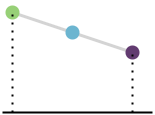
\includegraphics[width=0.5\textwidth]{img/pixel_verdopplung_graph.png}
            \caption{Graph über bilineare Skalierung.}
            \label{fig:graph_uber_bilineare_skalierung}
        \end{figure}

        Die bilineare Interpolation wird aufgrund ihrer Einfachheit und Effizienz häufig eingesetzt.
        Sie ist schnell zu implementieren und kann auf unterschiedliche Bildgrößen angewendet werden.
        Viele Bildbearbeitungssoftware und Grafikbibliotheken nutzen bilineare Interpolation als Standardmethode für die Skalierung von Bildern.
        Dennoch hat die bilineare Interpolation einige Nachteile, insbesondere bei extremen Skalierungen.
        Bei sehr großen oder kleinen Skalierungsfaktoren können Artefakte auftreten, die zu einer verminderten Bildqualität führen.
        In solchen Fällen können fortgeschrittenere Interpolationsverfahren wie Bicubic oder Lanczos eine bessere Wahl sein.


    \begin{figure}[h]
        \centering
        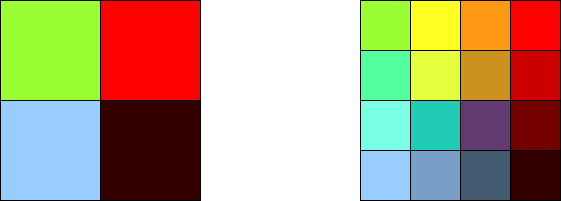
\includegraphics[width=0.5\textwidth]{img/pixel_verdopplung.png}
        \caption{Beispielgrafik zur Pixelverdopplung.}
        \label{fig:beispielgrafik_zur_pixelverdopplung}
    \end{figure}
    
    
    \begin{lstlisting}
    for y in range(self.new_height):
        for x in range(self.new_width):
            x_old = x / (self.new_width / self.width)
            y_old = y / (self.new_height / self.height)
    
            # Find the surrounding pixels
            x1 = int(x_old)
            x2 = min(x1 + 1, self.width - 1)
            y1 = int(y_old)
            y2 = min(y1 + 1, self.height - 1)
    
            # Check if x2 and y2 are out of bounds, if they are substract one
            if x2 == self.width - 1:
                x2 = x1
                x1 -= 1
            if y2 == self.height - 1:
                y2 = y1
                y1 -= 1
    
            # Find the weights
            w1 = (x2 - x_old) * (y2 - y_old)
            w2 = (x_old - x1) * (y2 - y_old)
            w3 = (x2 - x_old) * (y_old - y1)
            w4 = (x_old - x1) * (y_old - y1)
    
            # Get the pixel values of the surrounding pixels
            p1 = self.img.getpixel((x1, y1))
            p2 = self.img.getpixel((x2, y1))
            p3 = self.img.getpixel((x1, y2))
            p4 = self.img.getpixel((x2, y2))
    
            # Interpolate the pixel value
            new_pixel = (
                int(w1 * p1[0] + w2 * p2[0] + w3 * p3[0] + w4 * p4[0]),
                int(w1 * p1[1] + w2 * p2[1] + w3 * p3[1] + w4 * p4[1]),
                int(w1 * p1[2] + w2 * p2[2] + w3 * p3[2] + w4 * p4[2])
            )
            self.newImg.putpixel((x, y), new_pixel)
    \end{lstlisting}\footfullcite{1409828}
    
\section{Bikubische Interpolation}

\subsection{Mathematische Grundlagen}


% Erläuterung der mathematischen Grundlagen der bikubischen Interpolation, einschließlich der Verwendung von kubischen Polynomen und der Stichprobentheorie.
% Herleitung der bikubischen Interpolationsformel und der Eigenschaften der resultierenden Funktion.
% Diskussion der Vor- und Nachteile der Verwendung kubischer Funktionen für die Interpolation im Vergleich zu anderen Funktionstypen.
% Überblick über die Rolle der Fourier-Analyse und der Fourier-Transformationen bei der Bildinterpolation und wie sich dies auf die bikubische Interpolation bezieht.
    
Die bikubische Interpolation ist ein mathematisches Verfahren zur Schätzung der Werte einer kontinuierlichen Funktion an einer gegebenen Stelle, indem eine Funktion mit kubischen Polynomen verwendet wird, die durch benachbarte Funktionswerte verläuft.
Dabei wird das umliegende Gebiet untersucht und die Werte werden basierend auf der Stichprobentheorie geschätzt.

Die bikubische Interpolationsformel ist eine Erweiterung der Bilinearinterpolation auf vier umliegende Pixel und verwendet eine Funktion, die durch benachbarte Funktionswerte verläuft.
Die resultierende Funktion ist stetig differenzierbar und besitzt glatte partielle Ableitungen.

\begin{figure}[h]
    \centering
    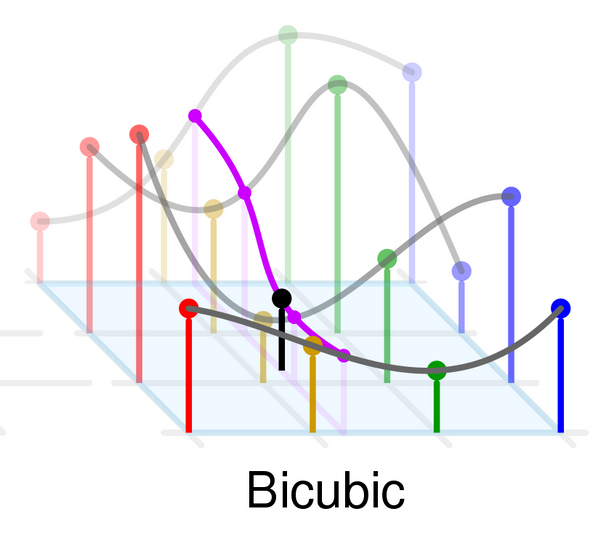
\includegraphics[width=0.5\textwidth]{img/bicubic_graph}
    \caption{Bikubische Interpolation}
    \label{fig:bicubic_interpolation}
\end{figure}

Im Vergleich zu anderen Interpolationsverfahren wie der bilinearen Interpolation und der Lanczos-Interpolation hat die bikubische Interpolation den Vorteil, dass sie eine höhere Genauigkeit bei der Schätzung von Pixelwerten bietet.
Ein Nachteil ist jedoch, dass sie im Allgemeinen höhere Rechenaufwendungen erfordert.

Die Fourier-Analyse und die Fourier-Transformationen spielen eine wichtige Rolle bei der Bildinterpolation, da sie es ermöglichen, die Funktion in den Frequenzraum zu transformieren und damit eine effektivere Interpolation zu erreichen.

\subsection{Algorithmische Implementierung}


% Überblick über die algorithmischen Schritte bei der bikubischen Interpolation, einschließlich der Auswahl der umgebenden Pixel und der Gewichte sowie der Berechnung der neuen Pixelwerte.
% Diskussion von Techniken zur Optimierung der Leistung der bikubischen Interpolation, wie z. B. die Vorberechnung von Lookup-Tabellen, Parallelisierung und Speicherverwaltung.
% Untersuchung von Grenzfällen und Randbedingungen, die bei der bikubischen Interpolation auftreten können, und wie diese effektiv behandelt werden können.
% Vergleich der algorithmischen Implementierung der bikubischen Interpolation mit anderen Interpolationsverfahren, wie z.B. der bilinearen Interpolation und der Lanczos-Interpolation.

    
Die bikubische Interpolation erfolgt durch die Auswahl von umgebenden Pixeln und deren Gewichte sowie der Berechnung der neuen Pixelwerte.

Sie verwendet eine 4x4-Matrix umliegender Pixel, um den Wert an einem bestimmten Punkt zu berechnen.
Die Formel zur Berechnung lautet:

Die Koeffizienten $a_{ij}$ werden basierend auf den umliegenden Pixelwerten und ihren Ableitungen berechnet.
Dieses Verfahren ermöglicht eine glatte Interpolation zwischen den Pixeln und hinterlasst wenige scharfe Kanten.

\begin{equation}
    f(x,y) = \sum_{i=0}^{3}\sum_{j=0}^{3}a_{i,j}*x^{i}*y^{j}
\end{equation}

Eine Möglichkeit zur Optimierung der Leistung besteht darin, Lookup-Tabellen vorzubereiten, Parallelisierungstechniken zu verwenden und die Speicherverwaltung zu optimieren.
Grenzfälle und Randbedingungen können bei der bikubischen Interpolation auftreten und müssen effektiv behandelt werden.
Die algorithmische Implementierung der bikubischen Interpolation kann mit anderen Interpolationsverfahren wie der bilinearen Interpolation und der Lanczos-Interpolation verglichen werden.

Ein Beispiel für die Implementierung der bikubischen Interpolation in Python ist der folgende Code:

Die Methode `manipulate` der Klasse `BicubicInterpolation` implementiert die bikubische Interpolation für das Vergrößern von Bildern.
Der wichtigste Teil des Codes ist die Schleife, die über jedes Pixel einen Kernel berechnet, der die jeweiligen Gewichte der benachbarten Pixel erechnet.
In den genannten Zeilen wird ein 4x4-Kern um das aktuelle Pixel herum gebildet und für jeden Pixel im Kern werden die Gewichte berechnet.
Dabei wird die `\_get\_weight`-Funktion aufgerufen, welche auf der Basis einer kubischen Kurve das Gewicht für einen bestimmten Abstand berechnet.
Die berechneten Gewichte werden in eine Liste `weights` hinzugefügt.
Diese Gewichte dienen später bei der Interpolation des aktuellen Pixels als multiplikative Faktoren für die umliegenden Pixel im Originalbild.


\begin{lstlisting}
weights = []
for j in range(-1, 3):
    for i in range(-1, 3):
        weight = _get_weight(i - dx) * _get_weight(dy - j)
        weights.append(weight)
\end{lstlisting}

\subsection{Analyse der Leistung}

    Zur Bewertung der Leistung von Bildinterpolationsverfahren werden verschiedene Kriterien verwendet, einschließlich der visuellen Qualität, der Genauigkeit und der Berechnungseffizienz. 
    Die Leistung der bikubischen Interpolation kann mit anderen Interpolationstechniken anhand von Testbildern und Datensätzen verglichen werden. 
    Dabei werden verschiedene Parameter wie Bildgröße, Auflösung und Inhalt untersucht, um ihre Auswirkungen auf die Leistung der bikubischen Interpolation zu analysieren. %...


% Ich hab das obere vom bot schreiben lassn

    \subsection{Implementation}
    \begin{lstlisting}
import math
from backend.image import Image

def _cubic(x, a=-0.5):
    abs_x = abs(x)
    if abs_x <= 1:
        return (a + 2) * (abs_x ** 3) - (a + 3) * (abs_x ** 2) + 1
    elif abs_x < 2:
        return a * (abs_x ** 3) - (5 * a) * (abs_x ** 2) + (8 * a) *
abs_x - (4 * a)
    return 0

def _get_weight(distance):
    abs_distance = abs(distance)
    if abs_distance <= 1:
        return _cubic(abs_distance)
    return 0

class BicubicInterpolation(Image):
    def __init__(self, path):
        extend = "biCu"
        super().__init__(path, extend)

    def manipulate(self, new_size):
        super().manipulate(new_size)

        for y in range(self.new_height):
            for x in range(self.new_width):
                px = x * self.width / self.new_width
                py = y * self.height / self.new_height

                ix = math.floor(px)
                iy = math.floor(py)

                dx = px - ix
                dy = py - iy

                weights = []
                for j in range(-1, 3):
                    for i in range(-1, 3):
                        weight = _get_weight(i - dx) * _get_weight(dy - j)
                        weights.append(weight)

                total_weight = sum(weights)
                normalized_weights = [w / total_weight for w in weights]

                new_pixel = [0, 0, 0]
                for j in range(-1, 3):
                    for i in range(-1, 3):
                        ox = ix + i
                        oy = iy + j
                        if ox < 0 or oy < 0 or ox >= self.width or
oy >= self.height:
                            pixel_value = list(
                                self.img.getpixel((min(max(ox, 0),
self.width - 1), min(max(oy, 0), self.height - 1)))
                            )
                        else:
                            pixel_value = list(self.img.getpixel(
(ox, oy)))

                        weight_index = (j + 1) * 4 + (i + 1)
                        weight = normalized_weights[weight_index]
                        for k in range(3):
                            new_pixel[k] += weight * pixel_value[k]

                self.newImg.putpixel((x, y), (int(new_pixel[0]),
int(new_pixel[1]), int(new_pixel[2])))

        return self.save()
    \end{lstlisting}


    \subsection{Anwendungen}

Die bikubische Interpolation wird in verschiedenen Anwendungen der Bildverarbeitung eingesetzt und bietet bestimmte Vorteile gegenüber der bilinearen Interpolation.
Ein Bereich, in dem die bikubische Interpolation besser geeignet sein kann, ist die Bildskalierung und -größenänderung.
Durch die Verwendung von zusätzlichen benachbarten Pixeln in der Interpolationsmethode kann die bikubische Interpolation feinere Details beibehalten und glattere Übergänge erzeugen, was zu hochwertigeren skalierten Bildern führen kann.

Ein weiterer Anwendungsbereich ist die Bildrotation und -transformation.
Bei der bikubischen Interpolation werden nicht nur benachbarte Pixel, sondern auch deren benachbarte Pixel berücksichtigt, wodurch eine bessere Anpassung an die gewünschten Rotationen oder Transformationen ermöglicht wird.
Dies kann zu weniger Verzerrungen und einem insgesamt realistischeren Ergebnis führen.

Die bikubische Interpolation kann auch in der Bildentrauschung und -wiederherstellung nützlich sein.
Durch die Verwendung von zusätzlichen Pixeln und einer gewichteten Interpolation können Rauschanteile reduziert und verloren gegangene Informationen wiederhergestellt werden.
Dies kann insbesondere in der medizinischen Bildgebung und der Satellitenbildgebung von Vorteil sein, wo genaue und zuverlässige Bilder erforderlich sind.

Wichtig zu beachten ist, dass die Eignung der bikubischen Interpolation von verschiedenen Faktoren abhängt, einschließlich der Natur des Eingangsbildes, des gewünschten Ausgabekontexts und der verfügbaren Rechenleistung.
In einigen Fällen kann die bikubische Interpolation aufgrund ihrer erhöhten Berechnungskosten und möglichen Unschärfen weniger geeignet sein.
Eine sorgfältige Bewertung der spezifischen Anforderungen und der verfügbaren Optionen ist daher umso entscheidender, um die optimale Interpolationsmethode für eine bestimmte Anwendung zu bestimmen.

    \subsection{Erweiterungen und Variationen}

    Erläuterung der verschiedenen Erweiterungen und Variationen der bikubischen Interpolation, wie z.
    B. Super-Resolution-Techniken, Multiskalen- und pyramidenbasierte Interpolation und adaptive Interpolationstechniken.
    Diskussion der Vor- und Nachteile dieser Varianten und ihrer Eignung für verschiedene Bildtypen und Anwendungen.
    Erkundung potenzieller künftiger Forschungsrichtungen in diesem Bereich, z.
    B. auf Deep Learning basierende Ansätze, ungleichmäßige und unregelmäßige Abtastverfahren sowie mehrdimensionale und mehrkanalige Interpolation.


\section{Lanczos-Interpolation}
    Die Lanczos-Interpolation ist eine Methode zur Rekonstruktion von Werten im Bild aus diskreten Abtastungen. 
    In diesem Abschnitt wird die mathematische Grundlage und die praktische Anwendung der Lanczos-Interpolation kurz erläutert.

\subsection{Mathematische Grundlage}

    Die Lanczos-Interpolation basiert auf der Idee, ein kontinuierliches Signal $f(x)$ durch eine Summe von gewichteten Basisfunktionen zu approximieren. 
    Dieses Signal können zum Beispiel Farbwerte in einem Bild sein.
    Die Basisfunktionen werden durch das sogenannte Lanczos-Kernel definiert:

\begin{equation}
    L(x) = \begin{cases} \frac{a \cdot \sin(\pi \cdot x) \cdot \sin(\pi \cdot x / a)}{(\pi \cdot x)^2} & \text{wenn } \left| x \right| < a \\ 0 & \text{sonst} \end{cases}
\end{equation}
~\footfullcite{duchon1979lanczos}

Das Lanczos-Kernel hat eine kompakte Trägerfunktion.
Eine kompakte Träägerformel bedeutet, sie ist nur in einem begrenzten Bereich von Null verschieden. 
In der Praxis hat dies den Vorteil, dass das Signalrauschen in Bereichen außerhalb des Bereichs im Signalraum reduziert wird und somit eine bessere Interpolation des Signals erreicht werden kann.
Die Gewichtungen der Basisfunktionen werden durch die Interpolationskoeffizienten bestimmt, die durch die diskreten Abtastungen des Signals berechnet werden.

Die Lanczos-Interpolation wird in der Regel auf gleichmäßig verteilten Stützstellen angewendet. 
Die Interpolationsmethode verwendet diese Stützstellen als Ausgangspunkt, um eine Schätzung des Signals an anderen Orten zu berechnen. 
Seien $x_1, x_2, \ldots, x_n$ die Stützstellen des Signals und $y_1, y_2, \ldots, y_n$ die zugehörigen Abtastungen.
Die Interpolationsfunktion $s(x)$ kann dann wie folgt berechnet werden:

\begin{equation}
    s(x) = \sum_{i=1}^{n} y_i \cdot L(x - x_i)
\end{equation}

Hierbei ist $L(x - x_i)$ die Lanczos-Kernel-Funktion, die den Beitrag des i-ten Stützpunkts zum interpolierten Signal an der Position x angibt.
Die Gewichtung erfolgt durch Multiplikation der Abtastung $y_i$ mit dem Wert des Lanczos-Kernels für den Abstand zwischen der Stützstelle $x_i$ und dem Zielpunkt x.

Die Wahl des Parameters $a$ beeinflusst die Schärfe der Interpolation.
Ein kleinerer Wert von $a$ führt zu einer breiteren Trägerfunktion und einer glatteren Interpolation, während ein größerer Wert von $a$ zu einer schärferen Trägerfunktion und einer detailreicheren Interpolation führt.
Es ist wichtig zu beachten, dass bei zu großen Werten von $a$ sogenannte Ringing-Artefakte auftreten können, bei denen sich unerwünschte Oszillationen um Kanten oder Kontrastübergänge im Bild bilden.

Insgesamt bietet die Lanczos-Interpolation eine effektive Methode zur Skalierung von Bildern mit Erhaltung von Details und Schärfe.
Sie ist jedoch rechenaufwändiger als einfachere Interpolationsmethoden, da sie eine Berechnung für jeden Pixel im skalierten Bild erfordert.
~\footfullcite{BENTBIB2016233}

\subsection{Praktische Anwendung}

Die Lanczos-Interpolation findet Anwendung in vielen Bereichen der Bildverarbeitung. 
Ein Anwendungsbeispiel ist die Upsampling von digitalen Bildern, um eine höhere Auflösung zu erreichen.

Die praktische Umsetzung der Lanczos-Interpolation erfordert die Berechnung der Interpolationskoeffizienten und die Bestimmung der Stützstellen des Signals. 
In der Regel werden hierfür spezielle Algorithmen eingesetzt, die auf der effizienten Berechnung der Basisfunktionen basieren.

\begin{lstlisting}
from backend.image import Image
import math

class LanczosInterpolation(Image):
    def __init__(self, path):
        extend = "lcz"
        super().__init__(path, extend)

    def lanczos_kernel(self, x, a=2):
        if x == 0:
            return 1
        elif abs(x) >= a:
            return 0
        else:
            return math.sin(math.pi * x) * math.sin(math.pi * x / a) /
(math.pi ** 2 * x ** 2)

    def manipulate(self, new_size):
        super().manipulate(new_size)

        for i in range(self.new_width):
            for j in range(self.new_height):
                x, y = i * self.width / self.new_width, j *
self.height / self.new_height
                u, v = math.floor(x), math.floor(y)
                s, t = x - u, y - v

                pixel = (0, 0, 0)
                weight_sum = 0

                for m in range(u - 2, u + 3):
                    for n in range(v - 2, v + 3):
                        if 0 <= m < self.width and 0 <= n < self.height:
                            weight = self.lanczos_kernel(s - (m - u)) *
self.lanczos_kernel(t - (n - v))
                            pixel = tuple([p + weight * self.img.getpixel(
(m, n))[i] for i, p in enumerate(pixel)])
                            weight_sum += weight
                if weight_sum > 0:
                    pixel = tuple([int(p / weight_sum) for p in pixel])
                    self.newImg.putpixel((i, j), pixel)

        return self.save()
\end{lstlisting}

\section{Zusammenfassung zu Vor- und Nachteilen von Techniken in der Bildverarbeitung}

In der Bildverarbeitung gibt es verschiedene Techniken, die verwendet werden können, um ein Bild zu bearbeiten oder zu manipulieren. 
In diesem Abschnitt werden wir uns mit einigen gängigen Techniken zur Interpolation von Bildern beschäftigen, nämlich Pixelverdopplung, Nearest Neighbour Interpolation, Bilineare Interpolation, Bikubische Interpolation und Lanczos Interpolation. 
Wir werden jeweils auf die Vor- und Nachteile dieser Techniken eingehen.

\subsection{Pixelverdopplung}

Bei der Pixelverdopplung wird jedes Pixel im Bild einfach dupliziert, um ein größeres Bild zu erzeugen. 
Diese Methode ist einfach und schnell, aber sie führt oft zu einer Verzerrung des Bildes und kann zu einer verschlechterten Bildqualität führen.

\subsection{Nearest Neighbour Interpolation}

Die Nearest Neighbour Interpolation ist eine einfache Interpolationsmethode, bei der jeder neue Pixelwert durch den nächstgelegenen Pixelwert im Originalbild bestimmt wird. 
Diese Methode ist einfach und schnell, aber sie führt oft zu einem "Treppeneffekt" im Bild, da die Pixelwerte nicht kontinuierlich interpoliert werden.

\subsection{Bilineare Interpolation}

Die bilineare Interpolation ist eine Methode, bei der die neuen Pixelwerte aus einer bilinearen Funktion berechnet werden, die aus den vier nächstgelegenen Pixeln im Originalbild abgeleitet wird. 
Diese Methode führt oft zu einer glatteren Interpolation als die Nearest Neighbour Interpolation, aber es kann immer noch zu einem "Verwischen" des Bildes kommen.

\subsection{Bikubische Interpolation}

Die bikubische Interpolation ist eine Methode, bei der die neuen Pixelwerte aus einer bikubischen Funktion berechnet werden, die aus den sechzehn nächstgelegenen Pixeln im Originalbild abgeleitet wird.
Diese Methode führt oft zu einer noch glatteren Interpolation als die bilineare Interpolation, aber sie kann auch zu einer Überbetonung von Bildstrukturen führen.

\subsection{Lanczos Interpolation}
Die Lanczos Interpolation ist eine Methode, bei der die neuen Pixelwerte aus einer Lanczos-Funktion berechnet werden, die aus einer begrenzten Anzahl von nächstgelegenen Pixeln im Originalbild abgeleitet wird. 
Diese Methode führt oft zu einer sehr glatten Interpolation und reduziert das Rauschen im Bild, aber sie kann auch zu einer gewissen Unschärfe im Bild führen.

\section{Analyse der Leistung}

    Erläuterung der Kriterien, die zur Bewertung der Leistung von Bildinterpolationsverfahren verwendet werden, einschließlich der visuellen Qualität, der Genauigkeit und der Berechnungseffizienz.

    Untersuchung der Auswirkungen verschiedener Parameter wie Bildgröße, Auflösung und Inhalt auf die Leistung der bikubischen Interpolation.
    Diskussion der potenziellen Einschränkungen und Kompromisse, die mit der Verwendung der bikubischen Interpolation verbunden sind, sowie der Faktoren, die ihre Leistung in verschiedenen Kontexten beeinflussen können.

    \begin{table}[h]
        \begin{tabular}{l|l|l|l}
            Verfahren & Geschwindigkeit & Qualität & Brauchbarkeit \\ \hline \hline
            Nearest Neighbour & schnell & mäßig & blockige Ergebnisse \\ \hline
            Bilineare Interpolation & mittel & gut & linearer Effekt \\ \hline
            Bicubische Interpolation & langsam & sehr gut & glättender Effekt \\ \hline
            Lanczos-Interpolation & langsam & sehr gut & glättender Effekt \\
        \end{tabular}
    \end{table}

Die Beurteilung von Bildinterpolationsverfahren erfolgt anhand diverser Kriterien, welche ihre Leistung charakterisieren.
Zu den frequent verwendeten Kriterien zählen die visuelle Qualität, die Genauigkeit sowie die Berechnungseffizienz.
Die visuelle Qualität bezieht sich auf die subjektive Wahrnehmung der Bildqualität nach der Interpolation.
Wesentliche Aspekte der visuellen Qualität beinhalten die Schärfe der Details, das Vorhandensein von Artefakten (z.B. Unschärfe oder Kantenartefakte) und die allgemeine Ästhetik des interpolierten Bildes.
Die Genauigkeit eines Interpolationsverfahrens betrifft dessen Fähigkeit, die tatsächlichen Werte oder Strukturen des Originalbildes möglichst präzise zu reproduzieren.
Eine präzise Interpolation minimiert den Informationsverlust und wahrt die inhärente Qualität des Bildes.
Die Berechnungseffizienz betrachtet die Laufzeit- und Ressourcenanforderungen des Interpolationsverfahrens.
Zügige und effiziente Methoden ermöglichen eine reibungslose Verarbeitung großer Datenmengen in Echtzeit oder bei der Stapelverarbeitung.

Beispiele aus dem wirklichen Leben umfassen Ladezeiten für Webseiten, medizinische Bildgebung oder Fernerkundung.
In wissenschaftlichen Anwendungen wie der medizinischen Bildgebung oder der Fernerkundung ist es von besonderer Bedeutung, dass präzise Messungen und Analysen durchführbar sind.
Eine präzise Interpolation minimiert den Informationsverlust und wahrt die inhärente Qualität des Bildes.
Die Berechnungseffizienz spielt eine ausschlaggebende Rolle in Anwendungen wie der Videokodierung oder der Echtzeitbildverarbeitung.

Es ist essenziell zu beachten, dass die Leistung der Interpolationsverfahren von diversen Faktoren abhängt, einschließlich der Bildgröße, der Auflösung, des Inhalts und des Kontextes der Anwendung.
Ein Verfahren, welches in einer bestimmten Situation gute Ergebnisse erzielt, kann in einer anderen Situation weniger erfolgreich sein.
Deshalb ist es wichtig, die spezifischen Anforderungen und Beschränkungen einer Anwendung zu berücksichtigen, um das am besten geeignete Interpolationsverfahren auszuwählen.

\subsection{Vergleich und Zusammenfassung}

Insgesamt gibt es keine "beste" Methode zur Interpolation von Bildern, da jede Methode ihre eigenen Vor- und Nachteile hat. 
Die Wahl der Methode hängt von den spezifischen Anforderungen und Einschränkungen ab, die für die jeweilige Anwendung gelten. 
Die Wahl einer geeigneten Interpolationsmethode kann jedoch die Bildqualität erheblich verbessern und zu einer effektiveren Bildverarbeitung führen.
\newpage



\chapter{Fortgeschrittene Skalierungsmethoden}

In diesem Kapitel werden fortgeschrittene Skalierungsmethoden behandelt.
Unter Beachtung der Erhaltung der Bildqualität werden Convolutional Neural Networks (CNNs) sowie Deep Learning zur Bildskalierung betrachtet.
Des Weiteren wird die Super Resolution vorgestellt.
Super Resolution ist eine Methode zur Generierung hochauflösender Bilder aus niedrigauflösenden Versionen, einschließlich der Wiederherstellung von verlorenen Details.

Ein weiterer Ansatz, ist der Einsatz von Generative Adversarial Networks (GANs), die durch den Wettbewerb zwischen einem Generator-Netzwerk und einem Diskriminator-Netzwerk hochrealistische Bilder erzeugen können.
Außerdem gibt es die Multiskalenskalierungstechnik, bei der verschiedene Skalierungsfaktoren angewendet werden, um eine ausgewogene Balance zwischen Details und Vergrößerung zu erreichen.
Abschließend werden die Vor- und Nachteile dieser fortgeschrittenen Methoden vorgestellt, um ein umfassendes Verständnis für ihre Anwendungsmöglichkeiten und Einschränkungen in der Bildverarbeitung zu entwickeln.


\section{Convolutional Neural Networks / Deep learning}
    \subsection{Grundlagen von Convolutional Neural Networks (CNNs)}
        Convolutional Neural Networks \ac{CNN} sind eine Art von Deep-Learning-Modell, welches besonders im Hinblick auf die Verarbeitung von Daten mit räumlicher Struktur den aktuellen Stand der Technik darstellt.      
        Räumliche Daten, wie z.B.      Bilder können bearbeitet, verarbeitet, erstellt und hauptsächlich analysiert werden.      
        CNNs bestehen aus mehreren Schichten von Neuronen, die so angeordnet sind, dass sie Merkmale extrahieren und Objekte Klassifizieren können.
        Die grundlegende Idee hinter CNNs ist die Verwendung von Faltung (engl.      convolution) zur Merkmalsextraktion und pooling layers.      
        Diese Art der Verbindung spart Rechenleistung und ermöglicht eine effektivere sowie schnellere Verarbeitung von großen Datensätzen\footfullcite{Li2022}.
        \footfullcite{kolbentwicklung,oshea2015introduction}
    \subsection{Architekturen von CNNs}
    
        Es gibt mehrere bekannte Architekturen von CNNs, darunter AlexNet\footfullcite{Aloysius2017}, ResNet\footfullcite{Pengcheng2020} und Inception\footfullcite{Zahangir2017}.

        \begin{figure}[h]
            \centering
            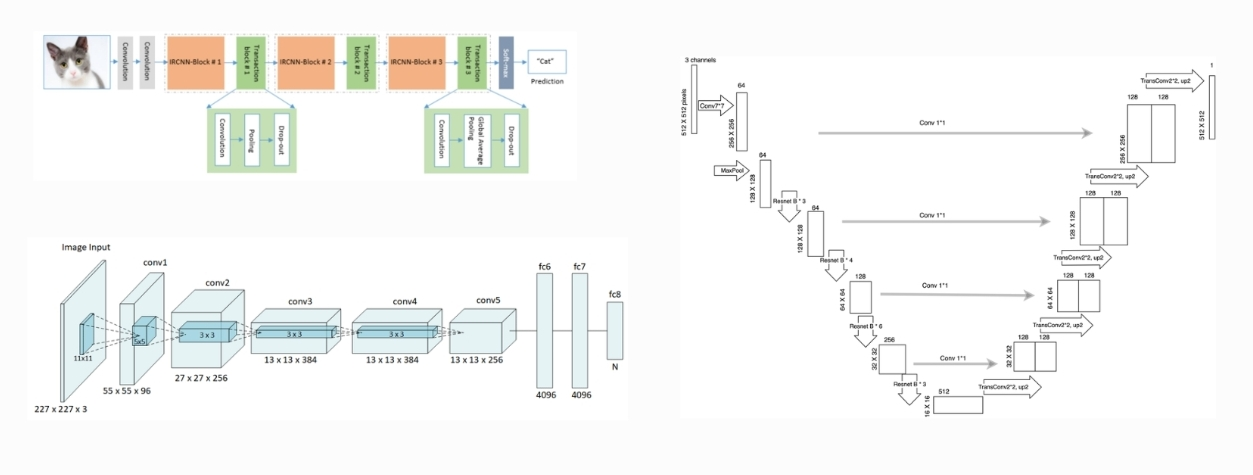
\includegraphics[width=0.8\textwidth]{img/different_types_of_cnn_nets.jpg}
            \caption{Verschiedene Architekturen von Image Networks. Oben links vereinfachtest Alex net, unten links inception net, rechts Abbildung der Res net Architektur.}
            \label{fig:my_label}
        \end{figure}
        
        AlexNet\footfullcite{Aloysius2017} war das erste CNN, das auf einem großen Datensatz erfolgreich angewendet wurde.
        ResNet zeichnet sich durch seine Fähigkeit aus, sehr tiefe Netzwerke zu trainieren, ohne dass das Problem des Verschwindens des Gradienten auftritt\footfullcite{Pengcheng2020}.  
        Inception wiederum ist für seine Fähigkeit bekannt, die Effizienz von CNNs durch die Verwendung von sogenannten Inception-Modulen zu erhöhen\footfullcite{Zahangir2017}.
        %TODO Grafiken für die Netzwerke raussuchen (BV Vorlesung?)

        \begin{figure}[h]
            \centering
            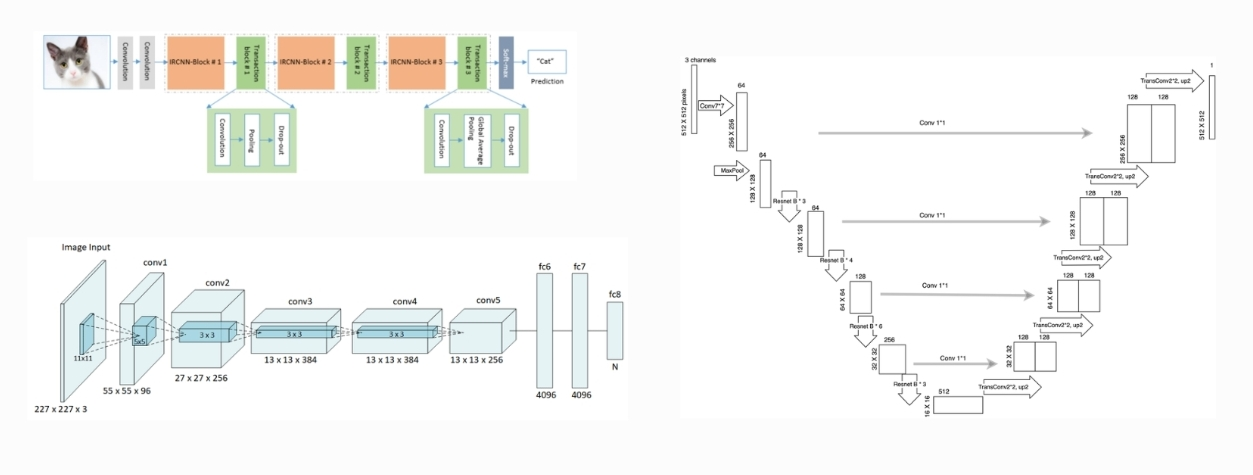
\includegraphics[width=0.8\textwidth]{img/different_types_of_cnn_nets.jpg}
            \caption{Verschiedene Architekturen von Image Networks. Oben links vereinfachtest Alex net, unten links inception net, rechts Abbildung der Res net Architektur.}
            \label{fig:my_label}
        \end{figure}
        
        AlexNet\footfullcite{Aloysius2017} war das erste CNN, das auf einem großen Datensatz erfolgreich angewendet wurde.
        ResNet zeichnet sich durch seine Fähigkeit aus, sehr tiefe Netzwerke zu trainieren, ohne dass das Problem des Verschwindens des Gradienten auftritt\footfullcite{Pengcheng2020}.  
        Inception wiederum ist für seine Fähigkeit bekannt, die Effizienz von CNNs durch die Verwendung von sogenannten Inception-Modulen zu erhöhen\footfullcite{Zahangir2017}.
    
    \subsection{Anwendungen von CNNs}
    
        CNNs haben zahlreiche Anwendungen, darunter Bildklassifizierung, Objekterkennung und Gesichtserkennung.      
        Bei der Bildklassifizierung werden Bilder automatisch in verschiedene Kategorien eingeteilt.      
        Beispielsweise können Bilder in Klassen wie Hunde, Katzen oder Autos eingeteilt werden.  
        Bei der Objekterkennung wird das Modell darauf trainiert, bestimmte Objekte in einem Bild zu erkennen, wie z.B.      Personen oder Straßenschilder.      
        Die Gesichtserkennung wird oft zur Identifikation von Personen in Sicherheitsanwendungen eingesetzt.
        \footfullcite{wu2017squeezedet,liu2015deep,jaderberg2015spatial}\footnote{\url{https://www.researchgate.net/figure/Object-detection-in-a-dense-scene_fig4_329217107}}

        \begin{figure}[h]
            \centering
            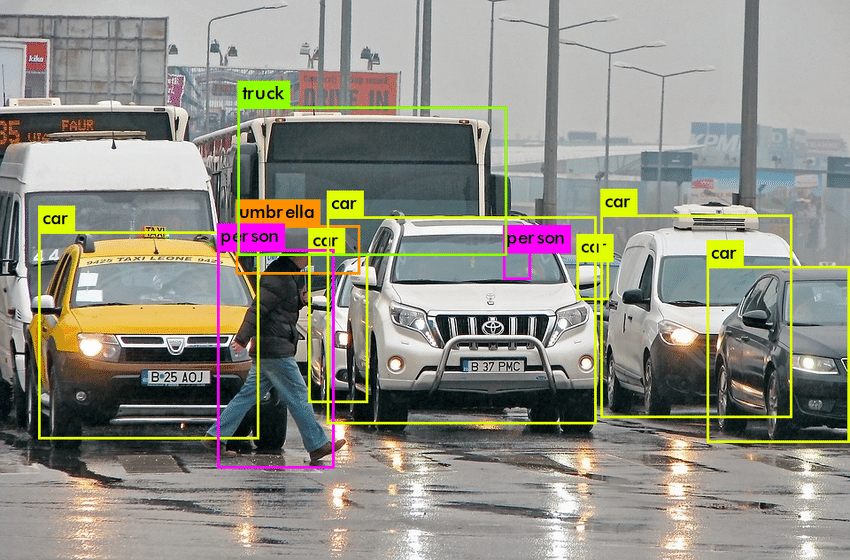
\includegraphics[width=0.6\textwidth]{img/Object-detection-in-a-dense-scene.ppm.png}
            \caption{Beispielbild eines Frames mit Bounding Boxes}
            \label{fig:Beispielbild_eines_Frames_mit_Bounding_Boxes}
        \end{figure}


    \subsection{Transfer Learning mit CNNs}
    
        Transfer Learning ist eine Technik, bei der ein bereits trainiertes CNN auf eine neue Aufgabe angewendet wird, ohne es von Grund auf neu zu trainieren.      
        Dies ist nützlich, wenn man nur über begrenzte Trainingsdaten verfügt oder wenn das Trainieren eines neuen Modells zu viel Zeit oder Ressourcen in Anspruch nimmt.      
        Ein Beispiel hierfür ist Erkennung von Autos, bei denen das Modell auf einem bereits trainierten CNN basieren kann, das auf z\.B\. Yolo v8 trainiert wurde\footfullcite{Nguyen2021}.

        In unserem Projekt haben wir das Modell resnet50 zur Trainingsgrundlage genommen, um unser eigenes Modell zu entwickeln. Wir haben den Code, den wir verwendet haben, um dieses Training durchzuführen, im Folgenden aufgeführt:

        \begin{lstlisting}
Net = torchvision.models.segmentation.deeplabv3_resnet50(pretrained=True)
        \end{lstlisting}

        Dieser Code\footnote{\url{https://github.com/studienarbeit-cnn-dhbwka-2022/Segmentation_cnn/blob/main/cnn.ipynb}} ermöglichte es uns, die Leistungsfähigkeit von resnet50 auszunutzen und es an unsere spezifischen Anforderungen anzupassen. Durch das Training unseres Modells konnten wir die gewünschten Ergebnisse erzielen und wichtige Erkenntnisse gewinnen, ohne ein Model von Grund auf zu trainieren.
        
    \subsection{Limitationen von CNNs und aktuelle Forschungsziele}

        Obwohl CNNs sehr erfolgreich bei der Verarbeitung von Bildern sind, haben sie auch einige Limitationen.      
        Zum Beispiel sind sie nicht gut geeignet, um komplexe Abhängigkeiten zwischen verschiedenen Eingabemerkmalen zu erfassen, wie z.B. das Verhalten von Objekten in einem Video.
        Zudem benötigen CNNs weiterhin viel Rechenleistung und Ressourcen
        \footfullcite{li2018visualizing}

        Facebooks Segment Anything Model (SAM) ist ein neues und Open-Source Modell, das sowohl interaktive als auch automatische Segmentierung durchführen kann.
        Die Benutzeroberfläche des Modells ermöglicht es, es auf flexible Weise zu verwenden, was eine Vielzahl von Segmentierungsaufgaben durch einfache Ingenieursarbeiten möglich macht.
        Das Modell wurde auf einem Datensatz von 11 Millionen Bildern und 1,1 Milliarden Masken trainiert und hat eine starke Null-Schuss-Leistung bei einer Vielzahl von Segmentierungsaufgaben\footnote{\url{https://research.facebook.com/publications/segment-anything/}}.

        \begin{figure}[h]
            \centering
            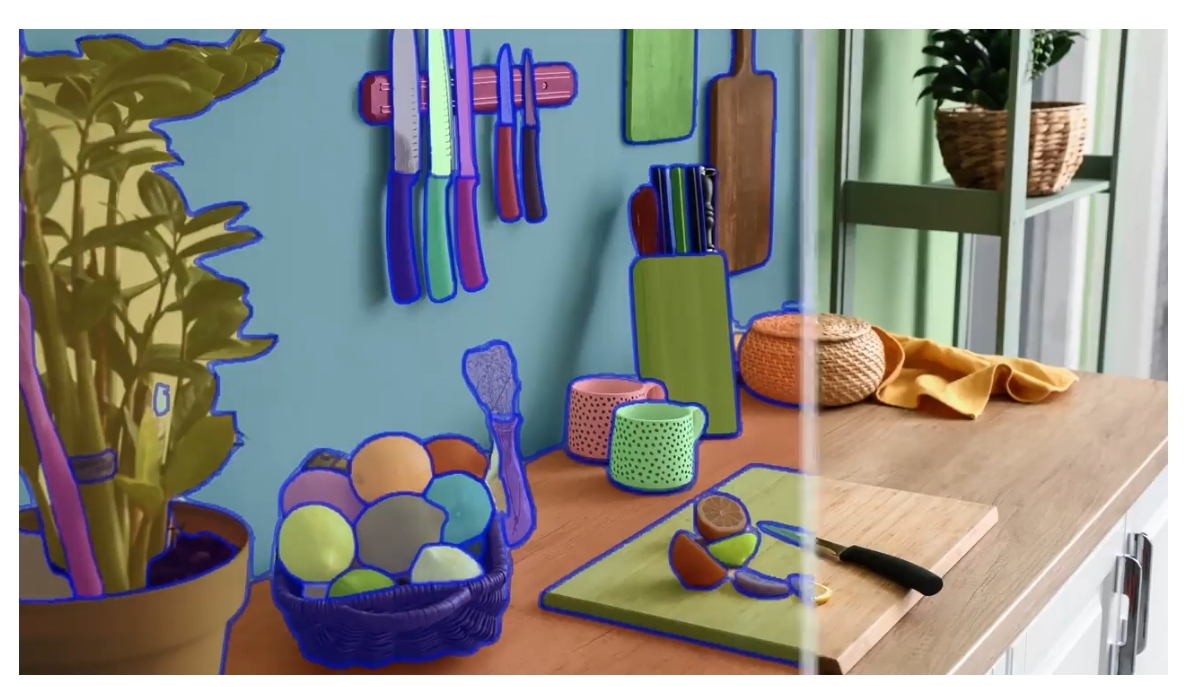
\includegraphics[width=0.6\textwidth]{img/SmartSelect_20230517_135035_Firefox.jpg}
            \caption{SAM: A generalized approach to segmentation}
            \label{fig:facebook_sam}
        \end{figure}

\section{Super Resolution}
    \subsection{Grundlagen von Super Resolution }
    
        Super Resolution \ac{SR} ist eine Technik, um aus einer niedrig aufgelösten Eingabe ein hochauflösendes Bild zu generieren.      
        Dies wird oft als Upscaling bezeichnet und findet in vielen Anwendungen wie der Bildrekonstruktion und Videoanalyse Anwendung.
        Die Grundidee hinter SR ist, dass hochauflösende Informationen in einem niedrig aufgelösten Bild versteckt sein können.      
        Die Herausforderung besteht darin, diese Informationen zu extrahieren und in ein hochauflösendes Bild zu integrieren.      
        SR ist somit ein Problem der inversen Bildgebung, bei dem eine hohe Auflösung aus einer niedrigen Auflösung abgeleitet werden muss.
        \footfullcite{7115171}
        
    \subsection{Super Resolution-Methoden auf Basis von Deep Learning}
    
        Super Resolution-Methoden auf Basis von Deep Learning haben in den letzten Jahren viel Aufmerksamkeit erhalten und sind derzeit der Stand der Technik für SR.      
        Diese Methoden verwenden Convolutional Neural Networks (CNNs) zur Verarbeitung von Bildern und zur Generierung von hochauflösenden Bildern.
        Es gibt verschiedene Arten von SR-Methoden auf Basis von Deep Learning, darunter Single-Image Super Resolution (SISR) und Multi-Image Super Resolution (MISR).      
        SISR-Methoden verwenden nur ein niedrig aufgelöstes Bild als Eingabe, während MISR-Methoden mehrere Bilder verwenden, um ein hochauflösendes Bild zu generieren.

        \begin{figure}[h]
            \centering
            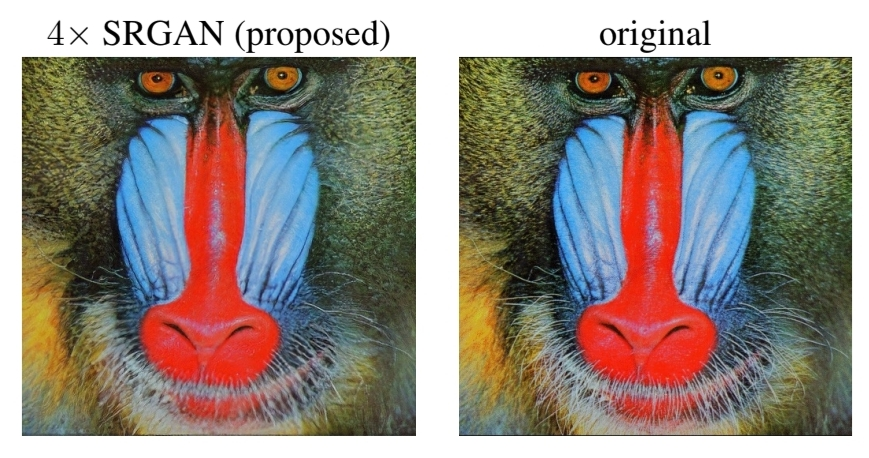
\includegraphics[width=0.7\textwidth]{img/SmartSelect_20230517_140120_Samsung Notes.jpg}
            \caption{Super resolution links, original rechts}
            \label{fig:superresolution}
        \end{figure}
        
        %TODO mehr auf sisr und misr eingehen hab ich aber nur semi verstanden so far 
    
    \subsubsection{Anwendungen von SR}
    
        SR hat viele Anwendungen in der Bild- und Videoanalyse, einschließlich der Rekonstruktion von Bildern aus medizinischen Scans, der Verbesserung von Bildern für die forensische Analyse\footfullcite{10.1007/978-0-387-73742-3_20} und der Verbesserung von Bildern für die Erkennung von Gesichtern und Objekten.
        In der Videoanalyse kann SR verwendet werden, um Videos zu stabilisieren, indem Bewegungsunschärfe reduziert und die Schärfe der Bilder verbessert wird.      
        SR kann auch bei der Entschlüsselung von unscharfen und verschwommenen Bildern in Überwachungsaufnahmen helfen.
    
    \subsubsection{Evaluierung von SR-Methoden}
    
        Die Evaluierung von SR-Methoden ist eine wichtige Aufgabe, um die Qualität und Effektivität der generierten Bilder zu bestimmen.      
        Die gängigen Evaluierungsmethoden umfassen die Verwendung von visuellen Qualitätsmetriken wie Peak Signal-to-Noise Ratio (PSNR) und Structural Similarity Index Measure (SSIM).
        Es gibt auch speziellere Evaluierungsmethoden wie die Verwendung von Perceptual Quality Assessment (PQA)-Maßnahmen, die menschliche Wahrnehmungseigenschaften berücksichtigen, um die Qualität der generierten Bilder zu bestimmen.
    
    \subsubsection{Herausforderungen und zukünftige Forschungsziele von Super Resolution}
    
        Obwohl SR-Methoden auf Basis von Deep Learning vielversprechende Ergebnisse erzielt haben, gibt es immer noch Herausforderungen und zukünftige Forschungsziele, die erforscht werden müssen.
        Eine der Herausforderungen besteht darin, dass SR-Methoden häufig dazu neigen, Artefakte in den generierten Bildern zu erzeugen, insbesondere bei der Verwendung von sehr hohen Upscaling-Faktoren.      %TODO Beispielbild Artefakte erklären
        Dies kann die visuelle Qualität der generierten Bilder beeinträchtigen und die Anwendbarkeit von SR-Methoden in bestimmten Szenarien einschränken.
        
        Eine weitere Herausforderung besteht darin, dass SR-Methoden häufig sehr rechenaufwändig sind, insbesondere wenn sie auf großen Datensätzen oder in Echtzeit angewendet werden müssen.      
        Die benötigten Ressourcen sind teuer.
        Dies kann die praktische Anwendbarkeit von SR-Methoden in einigen Anwendungen einschränken.        
        Zukünftige Forschungsziele könnten sich darauf konzentrieren, diese Herausforderungen zu überwinden, indem sie neue SR-Methoden entwickeln, die sowohl effektiv als auch effgizient sind.      
        Eine mögliche Lösung wäre die Verwendung von Generative Adversarial Networks (GANs) zur Verbesserung der visuellen Qualität der generierten Bilder und zur Reduzierung von Artefakten.      %TODO näher auf GAN eingehen 
        Eine weitere mögliche Lösung wäre die Entwicklung von neuartigen Architekturen von Deep Learning-Netzwerken, die weniger rechenaufwändig sind und schneller ausgeführt werden können\footfullcite{dong2016accelerating}\footfullcite{Park2020}.

        \subsubsection{Deep Learning Super Sampling}

        Eine vielversprechende Lösung zur Beschleunigung von Deep Learning ist Nvidia's DLSS-3 (Deep Learning Super Sampling 3, Stand 2023 Mai 17)\footnote{\url{https://www.nvidia.com/en-us/geforce/news/dlss3-ai-powered-neural-graphics-innovations/}}. 
        DLSS ist eine fortschrittliche Technologie, die von NVIDIA entwickelt wurde und es ermöglicht, hochauflösende Grafiken in Echtzeit zu rendern, indem es auf KI-Methoden basiert und durch Hardware (GPU) beschleunigt wird.
        DLSS bietet nicht nur schnellere Renderzeiten, sondern ermöglicht auch eine verbesserte Leistung auf Grafikkarten, da weniger rechenintensive Berechnungen erforderlich sind.
        Durch extensive Nutzung der CUDA cores, welche immer imposanter in Grafikarten eingebaut werden, ist das berechnen von Hohchauflösenden Bilder schneller mit jeder generation.
            
        % I want a tea party with Y'ha-nthlei

        ~
        
        Insgesamt bleibt SR ein aktives Forschungsfeld mit großem Potenzial für Anwendungen in der Bild- und Videoanalyse.      
        Mit weiteren Fortschritten in der Forschung können SR-Methoden immer leistungsfähiger und praktischer werden, um die Bedürfnisse der Industrie und der Geselllschaft zu erfüllen.

\section{Generative Adversarial Networks (GANs)}

    \subsection{Grundlagen von Generative Adversarial Networks (GANs)}
        
        Generative Adversarial Networks (GANs) sind ein leistungsstarkes Framework für das Training von Deep Learning-Modellen zur Generierung von Daten.      
        GANs bestehen aus zwei miteinander konkurrierenden neuronalen Netzwerken, einem Generator und einem Diskriminator.

        \begin{figure}[h]
            \centering
            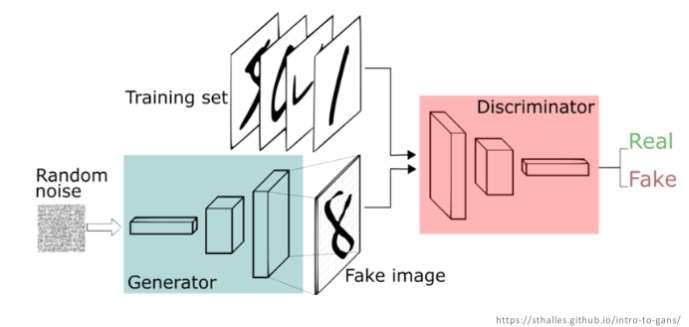
\includegraphics[width=0.7\textwidth]{img/GAN_architecture.jpg}
            \caption{Der Generator erzeugt neue Daten, während der Diskriminator versucht, zwischen den vom Generator erzeugten Daten und den echten Daten zu unterscheiden.}
            \label{fig:GAN_aufbau}
        \end{figure}
        
        Im Laufe des Trainings passt sich der Generator kontinuierlich an und verbessert seine Fähigkeit, realistische Daten zu generieren, während der Diskriminator gleichzeitig verbessert wird, um zwischen den generierten und echten Daten zu unterscheiden.
        %TODO GRAFIK! LUKAS! GRAFIK!
    
    \subsection{Architekturen von GANs}
    
        Es gibt verschiedene Architekturen von GANs, die für verschiedene Arten von Anwendungen geeignet sind.      
        in Beispiel ist das Deep Convolutional GAN (DCGAN), das speziell für die Generierung von Bildern entwickelt wurde.      %TODO Bild? ALso so architekkturbild oder so idk
        DCGAN nutzt Convolutional Neural Networks (CNNs) und Transposed Convolutional Neural Networks, um Bilder zu generieren, die visuell realistisch aussehen und strukturell konsistent sind.
        Ein weiteres Beispiel ist das CycleGAN\footfullcite{CycleGAN2017}, das für die Bildübersetzung zwischen verschiedenen Domänen verwendet werden kann.      
        CycleGAN nutzt einen Generator und einen Diskriminator sowie zusätzliche Cycle-Verlustfunktionen, um die Transformationen zwischen den Bildern in verschiedenen Domänen zu erlernen.%todo quellen vergessen
    
    \subsection{Anwendungen von GANs}
    
        GANs finden Anwendungen in verschiedenen Bereichen wie der Bildgenerierung, Style Transfer, der Verbesserung von Bildern und der Videoanalyse.      
        Zum Beispiel können GANs verwendet werden, um realistisch aussehende Bilder von Gesichtern, Landschaften oder anderen Objekten zu generieren.

        \begin{figure}[h]
            \centering
            
\includegraphics[width=0.4\textwidth]{img/cactus.jpg}
            \caption{Eingabe in das Modell: A small cactus wearing a straw hat and neon sunglasses in the Sahara desert.: \url{https://imagen.research.google/}}
            \label{fig:GAN_example}
        \end{figure}


        Style Transfer ermöglicht die Veränderung des visuellen Erscheinungsbildes von Bildern durch die Übertragung des Stils von einem Bild auf ein anderes.
        Dabei wird ein vortrainiertes neuronales Netzwerk verwendet, um Merkmale des Stils und Inhalts eines Bildes zu erfassen und zu kombinieren.
        Diese Technik hat Anwendungen in der Bildbearbeitung, Kunstgenerierung und visuellen Effekterstellung gefunden.
        
        Durch Style Transfer kann der visuelle Stil eines Bildes auf ein anderes übertragen werden, wobei ein vortrainiertes neuronales Netzwerk die Merkmale des Stils und Inhalts erfasst.
        Dies ermöglicht künstlerische Effekte und Anpassungen in der Bildbearbeitung und eröffnet neue Möglichkeiten für die kreative Gestaltung von visuellen Inhalten.

        Wie im dargestellten Bild zu sehen ist, wird das ursprüngliche Bild mithilfe des Stils des Gemäldes übertragen, wobei die Konturen des Hundes weiterhin erkennbar bleiben.

        \begin{figure}[h]
            \centering
            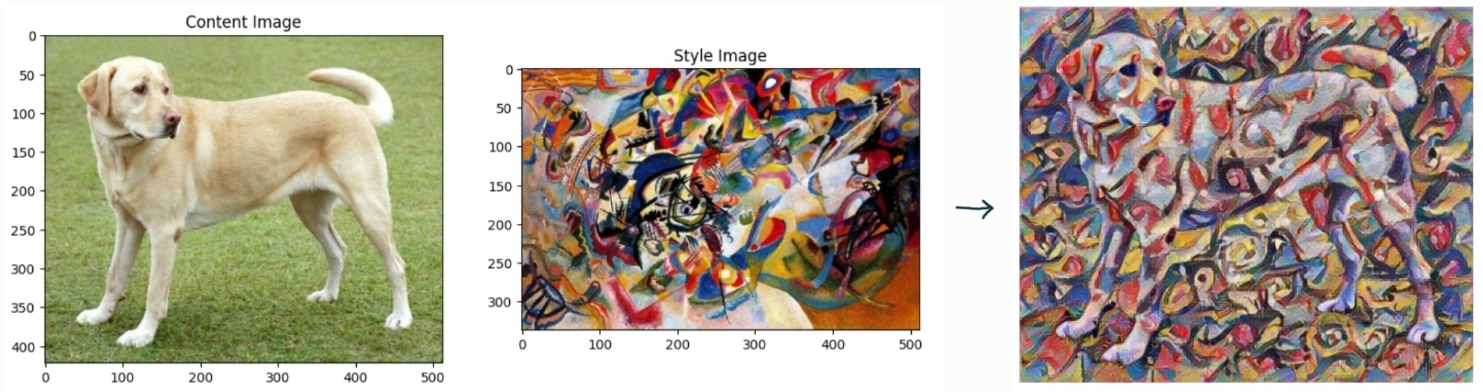
\includegraphics[width=0.9\textwidth]{img/GAN_style_trtansfer.jpg}
            \caption{\url{https://www.tensorflow.org/tutorials/generative/style_transfer}}
            \label{fig:GAN_style_transfer}
        \end{figure}
        
        GANs können auch verwendet werden, um Bilder mit höherer Auflösung oder besserer Qualität zu generieren, indem sie niedrig aufgelöste Bilder als Eingabe verwenden.
        GANs werden immer öfters in Bildverabreitungstools eingesetzt um fehlende Bereiche zu füllen, oder zum erweitern von Bildern (siehe \ref{fig:extend_image_imagen})\footnote{\url{https://imagen.research.google/}}.

        \begin{figure}[!h]
          \centering
          \begin{minipage}[b]{0.6\textwidth}
            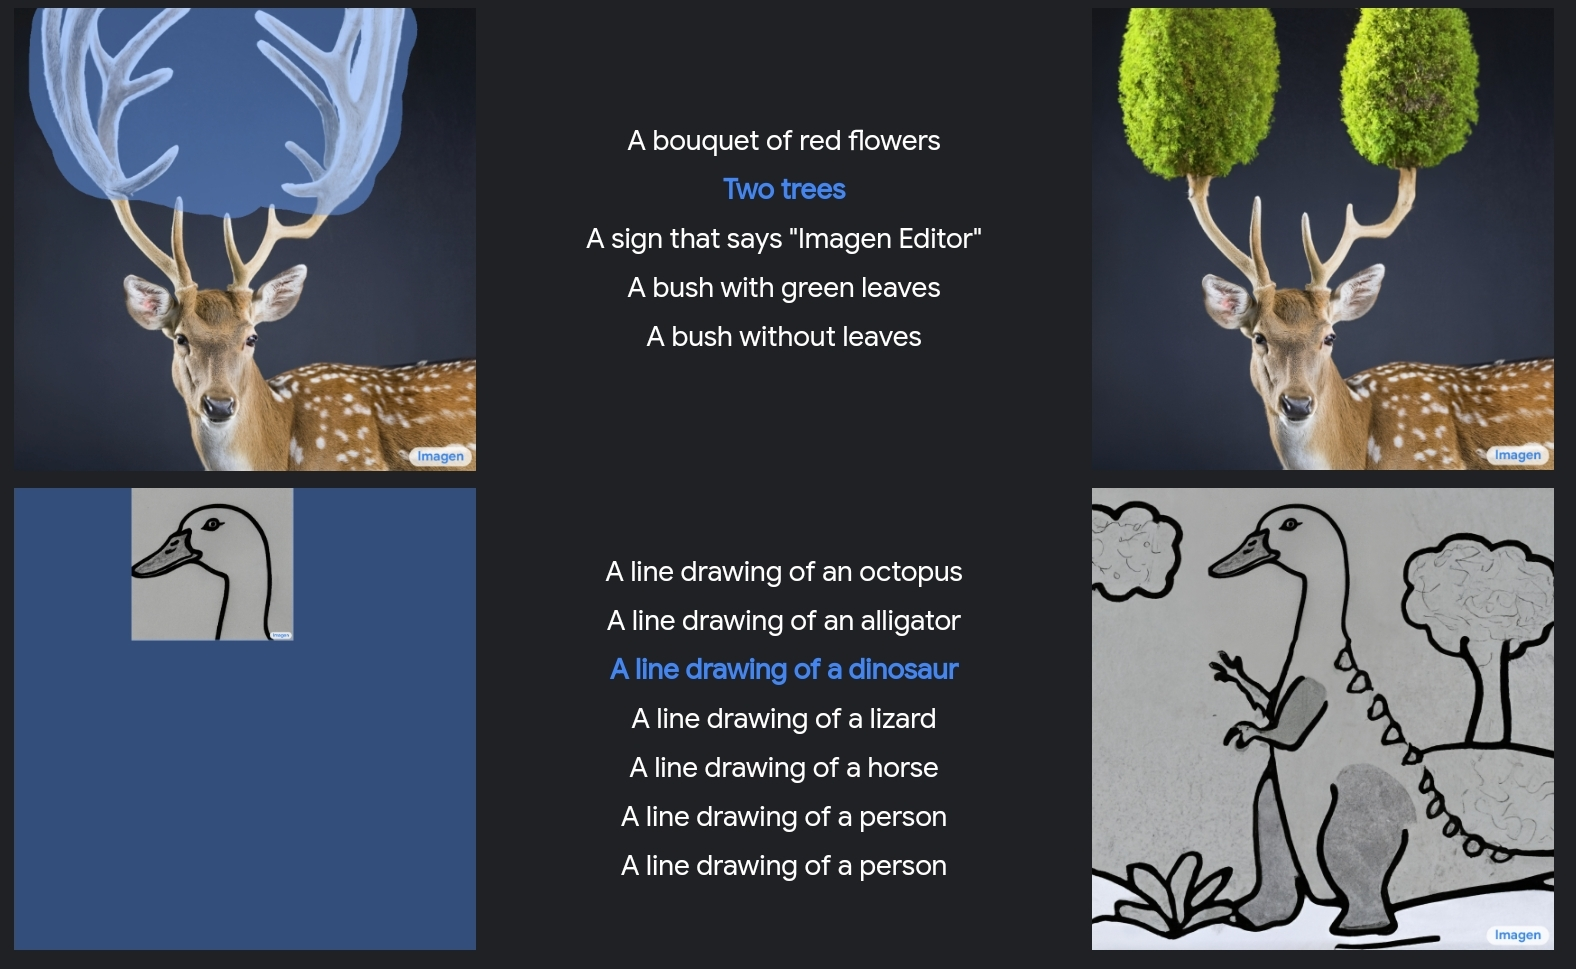
\includegraphics[width=\textwidth]{img/imagen_google_fill_and_extend.jpg}
          \end{minipage}
          \hfill
          \begin{minipage}[b]{0.35\textwidth}
            \caption{Füllen von markierten Bereichen eines Bildes durch verwendung von Imagen und Erweitern von Bildern mithilfe von Imagen, Google.}
          \end{minipage}
          \label{fig:extend_image_imagen}
        \end{figure}

        \newpage 
        % I cant deal with stupid latex anymore. Icant ocant icant

        In der Forschung können GANs verwendet werden, um Videosequenzen zu generieren oder zu verbessern. Ein modernes beispiel wäre Facebooks errungenschaften durch Make-A-Video\footnote{\url{https://ai.facebook.com/blog/generative-ai-text-to-video/}}, siehe \ref{fig:facebook_make_a_video}.

        \begin{figure}[!h]
            \centering
            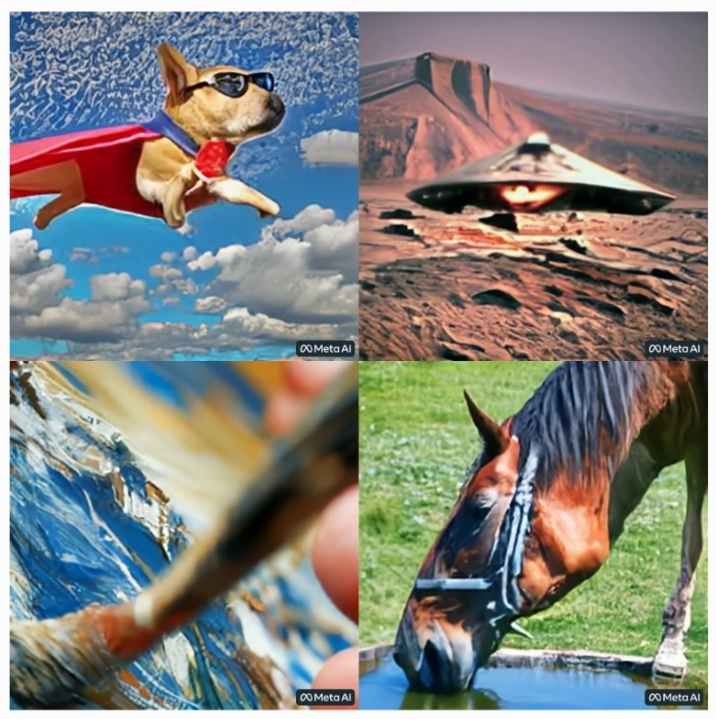
\includegraphics[width=0.6\textwidth]{img/facebook_make_a_video.jpg}
            \caption{Generierung kurzer Videos, anhand von sehr einfachen Beschreibungen.}
            \label{fig:facebook_make_a_video}
        \end{figure}
        
        Da wir leider nicht in Hogwards leben\footnote{Interaktive Zeitung aus Harry Potter: \url{https://youtu.be/xaBEFqFVSE8}}, können Videos \textit{nicht} auf PDFs angezeigt werden, noch weniger auf Papier. Die Eingaben für das Modell sind wie folgt: 
        Oben Links: A dog wearing a superhero cape flying through the sky.
        Oben rechts: A spaceship landing on Mars.
        Unten links: An artist's brush painting on a canvas close up, highly detailed. 
        Unten rechts: A horse drinking water.
        

    \subsection{Training von GANs und Evaluierung von generierten Ergebnissen}

        Das Training von GANs ist eine Herausforderung, da es sich um ein adversariales Lernverfahren handelt.      
        Das bedeutet, dass es zwei Netze gibt, die sich gegenseitig trainieren und verbessern.      %TODO Grafik & Quellen
        % Nö

        ~
        
        Das generative Netzwerk versucht, Bilder zu erzeugen, die von einem diskriminierenden Netzwerk nicht von echten Bildern unterschieden werden können.      
        Das diskriminierende Netzwerk wird trainiert, um echte Bilder von den vom generativen Netzwerk generierten Bildern zu unterscheiden.
        Das Training von GANs erfolgt durch die Minimierung einer Verlustfunktion, die als GAN-Verlust bezeichnet wird.

        ~
        
        Der GAN-Verlust besteht aus zwei Komponenten: dem Verlust des generativen Netzes und dem Verlust des diskriminierenden Netzes.      
        Der Verlust des generativen Netzes wird minimiert, wenn dasd Netzwerk Bilder erzeugt, die vom diskriminierenden Netzwerk nicht als gefälscht erkannt werden.      
        Der Verlust des diskriminierenden Netzes wird minimiert, wenn das Netzwerk in der Lage ist, besonders zuverlässig und schnell zwischen echten und generierten Bildern zu unterscheiden.
        Die Evaluierung von generierten Ergebnissen ist eine wichtige Aufgabe bei der Arbeit mit GANs.

~

        Es gibt verschiedene Methoden zur Bewertung von GANs, wie beispielsweise die visuelle Bewertung, die qualitative Bewertung und die quantitative Bewertung.  
        Die visuelle Bewertung beinhaltet das Betrachten der generierten Bilder, um zu beurteilen, ob sie realistisch aussehen oder nicht.      
        Die qualitative Bewertung beinhaltet die Verwendung von Bewertungsskalen, um die Qualität der generierten Bilder zu bewerten.      
        Die quantitative Bewertung beinhaltet die Verwendung von Metriken wie der Inception Score oder der Frechet Inception Distance, um die Qualität der generierten Bilder zu bewerten.

    \subsection{Ethische und soziale Implikationen von GANs}

    \begin{center}
        \textit{There are several ethical challenges facing text-to-image research broadly. We offer a more detailed exploration of these challenges in our paper and offer a summarized version here. First, downstream applications of text-to-image models are varied and may impact society in complex ways.}

        \url{https://imagen.research.google/}
    \end{center}
    
        Obwohl GANs eine vielversprechende Technologie sind, gibt es auch ethische und soziale Implikationen, die berücksichtigt werden müssen.      
        Ein Problem bei der Verwendung von GANs ist, dass sie zur Erzeugung gefälschter Bilder oder Videos verwendet werden können.      
        Dies kann zu Fälschungen und Manipulationen führen, die negative Auswirkungen auf die Gesellschaft haben können.
        Auch Rufschädigung kann durch GANs errleichtert werden.
        Ein weiteres Problem bei der Verwendung von GANs ist, dass sie möglicherweise nicht fair sind.  

        ~

        GANs können aufgrund ihrer Lernmethode unbewusste Vorurteile aufnehmen und in ihren generierten Ergebnissen widerspiegeln.      
        Dies kann zu diskriminierenden Ergebnissen führen, die unfaire Entscheidungen unterstützen.
        Es ist wichtig, dass bei der Verwendung von GANs Ethik und soziale Verantwortung berücksichtigt werden.      
        Es sollten Maßnahmen ergriffen werden, um sicherzustellen, dass GANs fair und ethisch korrekt arbeiten.      
        Zum Beispiel können spezielle Algorithmen entwickelt werden, um unbewusste Vorurteile zu minimieren.      
        Weiterhin können Regierungsbehörden und andere Organisationen Maßnahmen ergreifen, um den Missbrauch von GANs zu verhindern.   
        Das finden eines Kompromiss aus Forschung und politischer Einschränkung übersteigt jedoch den Rahmen dieser Arbeit.      
    
\section{Multiskalenskalierun}

    In vielen Anwendungen der Bildverarbeitung und Computergrafik ist es notwendig, Objekte oder Strukturen in verschiedenen Größenordnungen zu analysieren oder darzustellen.      
    Multiscale-Skalierung bezeichnet Techniken und Vorgehen, die es ermöglichen, Objekte oder Signale auf verschiedenen Skalen zu untersuchen oder zu manipulieren.      
    Dabei können sowohl lokale als auch globale Eigenschaften eines Objekts berücksichtigt werden.
    Diese Möglichkeiten komplementieren häufig Implementierungen von künstlichen Intelligenzen
    %TODO Zitat richtig einbauen

    \begin{center}
        \textit{Machine learning and multiscale modeling mutually complement one another.}\footfullcite{alber2019integrating}
    \end{center}
    
    \begin{center}
        \textit{Machine learning and multiscale modeling mutually complement one another.}\footfullcite{alber2019integrating}
    \end{center}
    
    \subsection{Grundlagen von Multiskalenskalierung}
    
        Multiscale-Skalierung ist ein Konzept aus der Signal- und Bildverarbeitung, das auf der Idee basiert, dass Signale und Bilder aus verschiedenen Skalen von Strukturen aufgebaut sind.
        In der Praxis bedeutet dies, dass ein Signal oder Bild auf verschiedene Skalen abgetastet oder transformiert wird, um Informationen auf verschiedenen Größenskalen zu erhalten.
        Ein grundlegendes Konzept der Multiscale-Skalierung ist die Skaleninvarianz.      
        Das bedeutet, dass die Informationen in einem Signal oder Bild unabhängig von der Skala erhalten bleiben sollten.      
        Das heißt, dass dieselben Merkmale oder Strukturen auf verschiedenen Skalen erkennbar sein sollten.
        \footfullcite{mallat1989theory,huang2017densely}
    
    \subsection{Methoden zur Multiskalenanalyse}
    
        Es gibt verschiedene Techniken zur Multiskalenanalyse, darunter Wavelet-Transformation und pyramidenartige Strukturen.      
        Wavelet-Transformation ist eine Methode zur Analyse und Synthese von Signalen oder Bildern auf verschiedenen Skalen.      
        Dabei wird das Signal oder Bild auf verschiedene Skalen und Frequenzen zerlegt, um Informationen auf verschiedenen Skalen zu erhalten.
        Pyramidenartige Strukturen sind eine weitere Methode zur Multiskalenanalyse, die in der Bildverarbeitung häufig verwendet wird.      
        Dabei wird das Signal oder Bild auf verschiedenen Skalen durch wiederholte Subsampling- und Filterungsoperationen reduziert.      
        Auf jeder Ebene der Pyramide wird das Signal oder Bild auf eine kleinere Größe reduziert, um Informationen auf verschiedenen Skalen zu erhalten.
        \footfullcite{burt1987laplacian,nah2017deep}
    
    \subsection{Methoden zur Multiskalenanalyse}
        Es gibt verschiedene Methoden zur Multiskalenanalyse, darunter Wavelets und Pyramiden.      
        Wavelets basieren auf der Zerlegung von Signalen in unterschiedliche Frequenzbänder, wodurch eine Multiskalenanalyse ermöglicht wird.      
        Eine Wavelet-Transformation kann auf ein Signal angewendet werden, um es in seine Hoch- und Niederfrequenzkomponenten zu zerlegen.      
        Diese Komponenten können dann unabhängig voneinander verarbeitet werden, um eine Analyse auf verschiedenen Skalen durchzuführen.
        Pyramiden sind eine weitere Methode zur Multiskalenanalyse, die auf der Idee der rekursiven Unterteilung von Signalen in immer feinere Skalen basiert.      Dabei wird ein Signal in eine Pyramide aus verschiedenen Ebenen unterteilt, wobei jede Ebene eine andere Skala darstellt.      
        Die unterste Ebene enthält das Originalsignal, während die oberen Ebenen eine immer gröbere Approximation des Signals enthalten.
        \footfullcite{simoncelli1996noise}
    
    \subsection{Anwendungen von Multiscale-Skalierung}
        Multiscale-Skalierung hat viele Anwendungen in der Bildverarbeitung und Computer Vision.
        Ein Beispiel ist die Texturanalyse, bei der Texturen auf verschiedenen Skalen analysiert werden, um Muster und Strukturen zu identifizieren.      
        Multiscale-Skalierung wird auch in der Bildkompression verwendet, um Bilder auf verschiedene Auflösungen zu skalieren und so Speicherplatz zu sparen.
        In jüngerer Zeit wurde die Multiskalenanalyse auch in Verbindung mit Deep Learning eingesetzt, um Modelle zu entwickeln, die auf verschiedenen Skalen arbeiten können.      
        Ein Beispiel ist das Multiscale Dense Network \ac{MSDN}, das eine skalierbare Architektur für die Bilderkennung bietet, die auf mehreren Skalen arbeiten kann.
    
    \subsection{Limitierungen und zukünftige Forschungsziele von Multiscale-Skalierung}
        Obwohl die Multiskalenanalyse in vielen Bereichen der Bildverarbeitung und Computer Vision erfolgreich eingesetzt wurde, gibt es auch einige Limitationen.  
        Eines der Hauptprobleme ist die Herausforderung, die richtige Skala für eine bestimmte Aufgabe zu wählen.      

        
        In einigen Fällen kann dies schwierig sein, da verschiedene Skalen unterschiedliche Informationen enthalten.
        Eine weitere Herausforderung besteht darin, die Multiskalenanalyse mit Deep Learning-Methoden zu integrieren.      
        Während einige Fortschritte in diesem Bereich gemacht wurden, gibt es immer noch Raum für Verbesserungen, um die Multiskalenanalyse nahtlos in Deep Learning-Architekturen zu integrieren\footfullcite{he2016deep}.
        
        Zukünftige Forschungsrichtungen könnten sich auf die Entwicklung von verbesserten Methoden zur Skalierung und Multiskalenanalyse konzentrieren, die eine höhere Genauigkeit und Effizienz ermöglichen.      
        Darüber hinaus könnten Forscher daran arbeiten, die Integration der Multiskalenanalyse in Deep Learning-Architekturen weiter zu verbessern, um noch bessere Ergebnisse zu erzielen.

\section{Vor- und Nachteile der fortgeschrittenen Methoden}

    Im Hinblick auf die Bildqualität sind Deep-Learning-basierte Methoden wie Super Resolution und GANs den traditionellen Methoden wie der Bilinear-Interpolation überlegen.      
    Diese Methoden können hochwertige Bilder mit hoher Auflösung und Details erzeugen, die den Originalbildern nahe kommen.      
    Insbesondere die GANs erlauben die Erzeugung von realistisch aussehenden Bildern, die schwer von echten Bildern zu unterscheiden sind.
    Ein weiterer Vorteil der fortgeschrittenen Methoden ist ihre Fähigkeit zur Generierung von neuen Inhalten.   
    So können GANs und Style Transfer genutzt werden, um neue Bilder zu erzeugen, die auf den Stil und Inhalt anderer Bilder basieren.      
    Dies bietet neue kreative Möglichkeiten in der Kunst und Design.

    Jedoch stellen diese fortgeschrittene Methoden auch Herausforderungen bei der Anwendung dar.      
    Beispielsweise benötigen Deep-Learning-Methoden große Datensätze und Rechenleistung, um optimal zu funktionieren\footfullcite{li2021beginner}.      
    Ein weiteres Problem ist die Interpretierbarkeit\footfullcite{he2023segmentation} der Ergebnisse, da es schwierig sein kann, zu verstehen, wie ein Modell zu seinen Ergebnissen gekommen ist.
    Die Anwendung von fortgeschrittenen Skalierungsmethoden hat auch Auswirkungen auf die Leistung und Effizienz von Systemen\footfullcite{Wang2018}.      
    So können Deep-Learning-basierte Methoden in Echtzeit-Anwendungen, wie beispielsweise autonomen Fahrzeugen, zu Verzögerungen führen.      
    Es ist daher wichtig, dass die Anforderungen an Leistung und Effizienz bei der Auswahl der Skalierungsmethode berücksichtigt werden.
    
    Es gibt moderne Architekturen und Techniken für höchst effiziente und leistungsstarke Ergebnisse.
    Zukunftsaussichten für fortgeschrittene Skalierungsmethoden liegen in der Kombination verschiedener Methoden. 
    So können beispielsweise GANs und Super Resolution zusammen genutzt werden, um qualitativ hochwertige und realistisch aussehende Bilder zu erzeugen.      
    Ein weiteres Forschungsgebiet ist die Verbesserung der Interpretierbarkeit und Erklärbarkeit von Deep-Learning-Modellen.      
    
    Insgesamt bieten fortgeschrittene Skalierungsmethoden in der Bildverarbeitung und Computergrafik viele Vorteile, jedoch müssen auch die Herausforderungen bei der Anwendung und die Auswirkungen auf die Leistung und Effizienz von Systemen berücksichtigt werden\footfullcite{Klver2022}.      
    Zukünftige Forschung sollte darauf abzielen, die verschiedenen Methoden zu kombinieren und die Interpretierbarkeit von Deep-Learning-Modellen zu verbessern.

\newpage


\chapter{Evaluation von Skalierungsmethoden}

\section{Qualitätsmetriken von Skalierungsmethoden}

    Die Evaluation von Skalierungsmethoden in der Bildverarbeitung bedarf einer facettenreichen Palette an Qualitätsmetriken, welche eine präzise Analyse und Vergleichbarkeit unterschiedlicher Methoden ermöglichen. 
    Im Rahmen dieser Arbeit werden ausgewählte sowie zentrale Qualitätsmetriken für die Bewertung von Skalierungsmethoden erörtert und diskutiert.

    \subsection{\ac{PSNR}}
        Das Peak Signal-to-Noise Ratio \ac{PSNR} ist eine der am häufigsten verwendeten Metriken zur Bewertung der Qualität von Bildern.
        Es misst die Qualität einer Bildrekonstruktion, indem es den Unterschied zwischen einem Originalbild und einem rekonstruierten Bild berechnet und diesen Unterschied durch das maximale Signal (Peak) und das Rauschen (Noise) im Originalbild teilt. 
        Je höher der PSNR-Wert, desto geringer ist der Unterschied zwischen Original- und Rekonstruktionsbildern und desto besser ist die Qualität der Rekonstruktion.
        \footfullcite{wang2004image}
        
        \subsubsection{Definition und Berechnung von \ac{PSNR}}
            Die Definition von PSNR lautet wie folgt:
            \begin{equation}
            PSNR = 20 \log_{10} \left( \frac{MAX_I}{\sqrt{MSE}} \right)
            %TODO prüf mal ob die Formel stimmt. Bin verzweifelt und hab die irwo aus stackoverflow geholt
            \end{equation}

            Dabei ist $MAX_I$ der maximal mögliche Pixelwert des Bildes.
            Bei der Darstellung von Pixeln mit 8 Bits pro Abtastwert ist dieser Wert 255.
            Allgemeiner ausgedrückt: Wenn die Samples mit linearer PCM mit B Bits pro Sample dargestellt werden, ist MAXI $2^B - 1$\footfullcite{wiki:Peak_signal-to-noise_ratio}.

            % wobei Peak der höchste mögliche Wert des Signals ist, der meist auf 255 bei 8-Bit-Graustufenbildern oder 65535 bei 16-Bit-Graustufenbildern gesetzt wird. %nur so semi verstanden aber die Quellen haben da ünbereingestimmt (stackoverflow help me)

            \begin{equation}
                MSE = \frac{1}{n*m} \sum_{i=0}^{n-1} \sum_{i=0}^{m-1} (I(i,j) - K(i,j))^2
            \end{equation}

            Der Mean Squared Error \ac{MSE} ist definiert als der Durchschnitt der quadrierten Unterschiede zwischen jedem Pixel des Originalbildes und dem rekonstruierten Bild.
            Je höher der PSNR-Wert, desto geringer ist der \ac{MSE} und desto besser ist die Qualität der Rekonstruktion.

        %TODO Quelle für Formel (wWill kein Stackoverflow link angeben) 
        \subsubsection{Anwendung von \ac{PSNR} bei der Bewertung von Bildqualität}
            Obwohl \ac{PSNR} eine weit verbreitete Methode zur Bewertung der Qualität von Bildern ist, hat sie auch ihre Limitationen\footfullcite{sheikh2006image}.
            Zum einen berücksichtigt sie nur die Fehler zwischen Original- und Rekonstruktionsbildern und vernachlässigt andere Faktoren wie Bildverzerrungen, die durch Komprimierung oder Filterung entstehen können.
            Zum andern ist der \ac{PSNR}-Wert nicht sensitiv für menschlich wahrgenommene Verzerrungen\footfullcite{mittal2012no}, wie z.B. Farbverschiebungen oder Artefakte.
            Trotz dieser Limitationen bleibt \ac{PSNR} eine wichtige Metrik in der Bildverarbeitung und wird oft in der Praxis verwendet, um die Qualität von Bildrekonstruktionen zu bewerten und zu vergleichen.
            \footfullcite{korhonen2012peak}
    \subsection{Structural Similarity Index Measure (SSIM)}

        Der Structural Similarity Index \ac{SSIM} ist eine Metrik zur Bewertung der strukturellen Ähnlichkeit zwischen einem Originalbild und einem rekonstruierten Bild.
        Im Gegensatz zum PSNR berücksichtigt der \ac{SSIM} nicht nur die Pixelwerte, sondern auch die Struktur und Textur des Bildes.
        Der \ac{SSIM} berechnet die Ähnlichkeit zwischen den beiden Bildern anhand von drei Faktoren: Helligkeit, Kontrast und Struktur. Die Formel zur Berechnung von \ac{SSIM} ist wie folgt:

        \begin{equation}
            \text{SSIM}(x, y) = \frac{{(2\mu_x\mu_y + c_1)(2\sigma_{xy} + c_2)}}{{(\mu_x^2 + \mu_y^2 + c_1)(\sigma_x^2 + \sigma_y^2 + c_2)}}
        \end{equation}

        In dieser Formel repräsentieren \(x\) und \(y\) zwei verglichene Bilder.
        Die \ac{SSIM} misst die strukturelle Ähnlichkeit zwischen diesen Bildern.
        \(\mu_x\) und \(\mu_y\) sind die Mittelwerte von \(x\) und \(y\), während \(\sigma_x^2\) und \(\sigma_y^2\) die Varianzen von \(x\) und \(y\) darstellen.
        \(\sigma_{xy}\) repräsentiert die Kovarianz zwischen \(x\) und \(y\).
        Die Konstanten \(c_1\) und \(c_2\) sind kleine Werte, die zur Stabilisierung der Division hinzugefügt werden
        \footfullcite{chen2011fast}\footfullcite{wiki:Structural_similarity}.


        \subsubsection{Anwendung von SSIM bei der Bewertung von Bildqualität}
        
            \ac{SSIM} wird häufig verwendet, um die Qualität von Bildrekonstruktionen zu bewerten. Es hat sich gezeigt, dass \ac{SSIM} besser als PSNR die wahrgenommene Bildqualität wiederspiegelt.
            Dies liegt daran, dass \ac{SSIM} die strukturelle Ähnlichkeit zwischen den beiden Bildern berücksichtigt, während \ac{PSNR} nur die Differenz der Pixelweite betrachtet.

        \subsubsection{Vorteile von SSIM im Vergleich zu PSNR}
        
            Im Vergleich zum \ac{PSNR} hat \ac{SSIM} mehrere Vorteile. Zum einen berücksichtigt es die strukturelle Ähnlichkeit zwischen den beiden Bildern, was zu einer besseren Bewertung der wahrgenommenen Bildqualität führt.
            Zum anderen ist \ac{SSIM} in der Lage, Verzerrungen zu erkennen, die durch Kompression oder andere Arten von Bildverarbeitung verursacht werden, während \ac{PSNR} dies nicht tut.
        \footfullcite{5596999}
        
        \subsubsection{Limitationen von SSIM}
        
            Obwohl \ac{SSIM} eine bessere Metrik zur Bewertung der Bildqualität als \ac{PSNR} darstellt, hat es auch seine Limitationen.
            \ac{SSIM} ist anfällig für Helligkeits- und Kontrastunterschiede zwischen den beiden Bildern und kann bei der Bewertung von stark komprimierten Bildern ungenau sein.
            Auch bei der Anwendung auf Bilder mit unterschiedlichen Strukturen kann die \ac{SSIM} eine ungenaue Bewertung liefern.
        \footfullcite{1284395}
    \subsection{Mean Opinion Score (MOS)}
        Der Mean Opinion Score \ac{MOS} ist eine subjektive Metrik, die die wahrgenommene Qualität einer Bildrekonstruktion misst.
        MOS basiert auf der Bewertung durch menschliche Beobachter, die gebeten werden, die Qualität von Original- und Rekonstruktionsbildern auf einer Skala von 1 bis 5 oder 1 bis 10 zu bewerten.
        MOS ist eine wichtige Metrik, da sie die subjektive Wahrnehmung der Qualität eines Bildes durch den Betrachter berücksichtigt.
        \footfullcite{sheikh2006image}
        
    \subsection{Peak Signal-to-Noise Ratio der Y-Komponente (PSNR-Y)}
        Die Y-Komponente im YCbCr-Farbraum enthält die Helligkeitsinformationen des Bildes. 
        Das Peak Signal-to-Noise Ratio der Y-Komponente \ac{PSNR-Y} ist eine spezielle Version des \ac{PSNR}, die nur die Helligkeitsinformationen des Originalbildes und des rekonstruierten Bildes berücksichtigt.
        \ac{PSNR}-Y ist eine wichtige Metrik zur Bewertung der Qualität von Skalierungsmethoden für Graustufen- oder Schwarz-Weiß-Bilder.
        Diese Qualitätsmetriken sind wichtigeWerkzeuge für diew Bewertung und den Vergleich von Skalierungsmelthoden in der Bildverarbeitung.
        Es ist jedoch wichtig zu beachten, dass keine einzelne Metrik alle Aspekte der Bildqualität abdeckt. Eine umfassende Bewertung sollte mehrere Metriken kombinieren und auch die subjektive Wahrnehmung 
        \footfullcite{huang2010new}
        
    \subsection{Computational Speed}
    
        Die Wahl einer Skalierungsmethode hängt nicht nur von der Bildqualität, sondern auch von der benötigten Rechenleistung ab. 
        Die Computational Speed ist daher ein wichtiger Faktor bei der Auswahl einer Skalierungsmethode.
        Es gibt verschiedene Methoden zur Messung von Computational Speed, wie z.B. die Messung der benötigten Zeit, um ein Bild zu skalieren oder die Berechnung von \ac{FLOPS}. 
        Eine genauere Messung kann durch die Verwendung von Benchmarks erreicht werden, die es ermöglichen, verschiedene Skalierungsmethoden auf derselben Hardware zu vergleichen.
        Jedoch muss bei der Messung der Computational Speed berücksichtigt werden, dass die Leistung des verwendeten Computers die Ergebnisse beeinflussen kann. 
        Ein schnellerer Computer kann eine Methode schneller ausführen als ein langsamerer Computer. 
        Daher ist es wichtig, die Messungen auf einem vergleichbaren Computer durchzuführen und die Ergebnisse zu normalisieren.
        Ein wichtiger Trade-off besteht zwischen der Bildqualität und der Computational Speed. 
        Eine Methode, die eine höhere Bildqualität liefert, benötigt in der Regel mehr Rechenleistung und ist daher langsamer als eine Methode mit niedrigerer Bildqualität. 
        Es ist daher wichtig, die gewünschte Bildqualität und die verfügbare Rechenleistung abzuwägen und eine Methode zu wählen, die den Anforderungen am besten entspricht. 
        Es können auch Techniken wie progressiver Skalierung verwendet werden, um eine gute Bildqualität mit einer angemessenen Geschwindigkeit zu erreichen.
        \footfullcite{xu2017efficient,choi2019lightweight}
        
    \subsection{Root-Mean-Square Error (RMSE)}
    
        Der Root-Mean-Square Error \ac{RMSE} ist eine Metrik zur Bewertung der Qualität von Bildrekonstruktionen. 
        Ein Nachteil von RMSE ist, dass er nur den Fehler zwischen Pixelwerten betrachtet und keine Berücksichtigung von strukturellen Unterschieden im Bild nimmt. 
        Daher wird RMSE oft in Kombination mit anderen Metriken wie \ac{PSNR} und \ac{SSIM} verwendet, um ein umfassenderes Bild der Bildqualität zu erhalten.
        Abschließend ist zu sagen, dass beider Bewertung von Bildqualität die Wahl der Metrik von der spezifischen Anwendung abhängt. 
        Während \ac{PSNR} und \ac{SSIM} für die Bewertung von Bildern in vielen Anwendungen ausreichend sein können, kann in anderen Fällen die subjektive Wahrnehmung des menschlichen Betrachters durch MOS eine bessere Metrik sein.
        Darüber hinaus ist bei der Wahl einer Skalierungsmethode auch die Messung von Computational Speed und das Abwägen von Trade-offs zwischen Bildqualität und Geschwindigkeit von entscheidender Bedeutung.
        \footfullcite{morad1996role}
        
\section{Kriterien zur Auswahl der Skalierungsmethode} %TODO Hier können wir viele Bilder einbauen um die Vergleichsgrafiken besser zu erklären (@MARC)

    \subsection{Bildvergleich und visuelle Bewertung}
        
        Die Evaluation von Skalierungsmethoden in der Bildverarbeitung erfordert eine umfassende und präzise Analyse verschiedener Kriterien, um die optimale Methode auszuwählen. 
        Ein wesentlicher Aspekt bei dieser Bewertung ist der Bildvergleich und die visuelle Bewertung, die auf der subjektiven Wahrnehmung von menschlichen Beobachtern beruhen.
        Die visuelle Bewertung von Bildern durch menschliche Beobachter ermöglicht eine direkte und subjektive Beurteilung der Bildqualität basierend auf wahrgenommenen visuellen Eigenschaften. 
        Verschiedene Methoden des Bildvergleichs werden eingesetzt, wie beispielsweise der Side-by-Side-Vergleich, bei dem zwei Bilder direkt miteinander verglichen werden, oder der Triple-Stimulus-Test, bei dem ein Originalbild mit zwei rekonstruierten Bildern verglichen wird.
        Diese Methoden des Bildvergleichs und der visuellen Bewertung werden auch bei der Evaluierung von Skalierungsmethoden angewendet. 
        Durch den Vergleich der rekonstruierten Bilder mit dem Originalbild können verschiedene Skalierungsmethoden anhand ihrer visuellen Qualität beurteilt und verglichen werden. 
        dies ermöglicht eine umfangreiche Analyse und eine direkte Gegenüberstellung der unterschiedlichen Methoden.
        Es ist jedoch von entscheidender Bedeutung, die Limitationen und Vorbehalte im Zusammenhang mit der visuellen Bewertung von Bildern zu berücksichtigen. 
        Die subjektive Wahrnehmung kann von Person zu Person variieren und wird auch von anderen Faktoren wie Beleuchtung, Betrachtungsabstand und individuellen Präferenzen beeinflusst. 
        Darüber hinaus können komplexe visuelle Verzerrungen nicht immer präzise durch die visuelle Bewertung erfasst werden. 
        Daher sollten bei der Bewertung von Skalierungsmethoden auch objektive Metriken und weitere Evaluierungskriterien einbezogen werden.
        Insgesamt spielt der Bildvergleich und die visuelle Bewertung eine bedeutende Rolle bei der Evaluierung von Skalierungsmethoden in der Bildverarbeitung.
        Durch die Kombination der subjektiven visuellen Bewertung mit objektiven Metriken können fundierte Entscheidungen getroffen werden, um die optimale Methode gemäß den spezifischen Anforderungen der Anwendung auszuwählen. 
        Die sorgfältige Berücksichtigung der genannten Limitationen trägt dazu bei, zuverlässige und aussagekräftige Ergebnisse zu erzielen und die Qualität von Bildrekonstruktionen bestmöglich zu bewerten.
        \footfullcite{ye2012no,wang2004image,eckert1998perceptual}
    
    \subsection{Effektivität und Effizienz}

        Die Bewertung von Skalierungsmethoden in der Bildverarbeitung erfordert eine umfassende Betrachtung sowohl der Effektivität, also der Bildqualität, als auch der Effizienz, insbesondere der Computational Speed. 
        Es besteht ein inhärenter Trade-off zwischen der erzielten Bildqualität und der benötigten Rechenleistung, der bei der Auswahl der optimalen Skalierungsmethode berücksichtigt werden muss.
        Die Effektivität einer Skalierungsmethode bezieht sich auf die erzielte Bildqualität der rekonstruierten Bilder. 
        Eine Methode, die eine höhere Bildqualität liefert, wird in der Regel auch mehr Rechenleistung benötigen und somit langsamer sein als eine Methode mit geringerer Bildqualität. 
        Daher ist es von großer Bedeutung, die gewünschte Bildqualität und die verfügbare Rechenleistung sorgfältig abzuwägen, um die beste Skalierungsmethode zu wählen.


        \begin{table}[!h]
        \centering
        \begin{tabular}{ccccccc}
            \textbf{Model} & \textbf{PLCC} & \textbf{MAE} & \textbf{RMS} & \textbf{SRCC} & \textbf{KRCC} & \textbf{Computation time} \\ \hline
            PSNR           & 0.9062        & 7.4351       & 9.8191       & 0.8804        & 0.6886        & 1                                     \\
            SSIM           & 0.9253        & 6.9203       & 8.8069       & 0.9014        & 0.7246        & 22.65                                 \\
            MS-SSIM        & 0.8945        & 8.1969       & 10.384       & 0.8619        & 0.6605        & 48.49                                 \\
            SSIMplus       & 0.9732        & 4.3192       & 5.3451       & 0.9349        & 0.7888        & 7.83
        \end{tabular}
        \caption{Leistungsvergleich zwischen PSNR, SSIM, MS-SSIM, VQM, PQR-Tek, DMOS-Tek, JND-VC,
DMOS-VC und SSIMplus einschließlich aller Geräte\footfullcite{Rehman_Zeng_Wang_2015}.}
        \label{tab:Leistungsvergleich}
        \end{table}



        Die Evaluierung der Trade-offs zwischen Effektivität und Effizienz erfordert eine gründliche Analyse der Leistungsmerkmale verschiedener Skalierungsmethoden.
        Hierbei können Kosten-Nutzen-Analysen hilfreich sein, um die Auswirkungen der gewählten Methode auf die Bildqualität und die erforderliche Rechenleistung abzuschätzen. 
        Indem die Kosten in Bezug auf die erzielte Bildqualität bewertet werden, kann die optimale Methode entsprechend den spezifischen Anforderungen des Anwendungsbereichs ausgewählt werden.
        Die Relevanz von Effektivität und Effizienz variiert je nach Anwendungsbereich der Bildverarbeitung. 
        In einigen Fällen, wie beispielsweise medizinischen Bildgebungsverfahren oder hochauflösenden Videoanwendungen, ist eine hohe Bildqualität von größter Bedeutung, selbst wenn dies mit einem höheren Rechenaufwand einhergeht. 
        In anderen Szenarien, wie in Echtzeit-Anwendungen oder mobilen Geräten, kann die Effizienz und die schnelle Verarbeitung der Bilder priorisiert werden, auch wenn dies zu einer gewissen Einbuße der Bildqualität führt.
        Insgesamt ist es von entscheidender Bedeutung, sowohl die Effektivität als auch die Effizienz bei der Wahl der besten Skalierungsmethode zu berücksichtigen. 
        Die richtige Balance zwischen Bildqualität und erforderlicher Rechenleistung zu finden, ermöglicht die optimale Nutzung von Ressourcen und die Erfüllung der spezifischen Anforderungen des jeweiligen Anwendungsbereichs der Bildverarbeitung.
        \footfullcite{zhang2019efficiency}\footfullcite{gu2019comprehensive}\footfullcite{hu2020efficient}

    \subsection{Zukunftsaussichten und Herausforderungen}
    
        Die kontinuierliche Entwicklung von Technologien stellt neue Herausforderungen bei der Evaluierung von Skalierungsmethoden in der Bildverarbeitung dar.
        Fortschritte in der Hardware, wie leistungsstärkere Prozessoren und spezialisierte Beschleuniger, können die Rechenleistung erhöhen und somit neue Möglichkeiten für komplexe Skalierungsalgorithmen eröffnen. Gleichzeitig führen neue Technologien wie Virtual Reality, Augmented Reality und 8K-Bildschirme zu höheren Anforderungen an die Bildqualität und erfordern präzisere Bewertungsmethoden.
        Spezifische Anwendungsbereiche, wie die medizinische Bildgebung oder die Videokompression, stellen weitere Herausforderungen bei der Evaluierung von Skalierungsmethoden dar. 
        In der medizinischen Bildgebung ist die genaue Beurteilung der Bildqualität von entscheidender Bedeutung für die richtige Diagnosestellung und Behandlungsplanung. 
        Hier müssen spezielle Metriken und Evaluierungsverfahren entwickelt werden, um den Anforderungen dieses Bereichs gerecht zu werden. 
        Ebenso erfordert die Videokompression eine sorgfältige Evaluierung der Skalierungsmethoden, um eine ausreichende Qualität der komprimierten Videos zu gewährleisten und gleichzeitig die Effizienz der Kompression zu maximieren.
        Ein vielversprechendes Potenzial für die zukünftige Evaluierung von Skalierungsmethoden liegt in der Anwendung von KI-basierten Evaluierungsmethoden. 
        Durch den Einsatz von maschinellem Lernen und neuronalen Netzwerken können automatisierte Bewertungsalgorithmen entwickelt werden, die die menschliche Wahrnehmung von Bildqualität besser simulieren. 
        Diese KI-basierten Ansätze können eine schnellere und objektivere Evaluierung ermöglichen und den Entwicklungsprozess von Skalierungsmethoden beschleunigen.
        Bei der Bewertung von Skalierungsmethoden sollten jedoch auch ethische und soziale Implikationen berücksichtigt werden. 
        Die Entwicklung von immer leistungsfähigeren Skalierungsmethoden kann auch potenzielle Risiken mit sich bringen, wie zum Beispiel die Manipulation von Bildern oder die Schaffung von gefälschten Inhalten. 
        Es ist daher wichtig, entsprechende Schutzmechanismen zu entwickeln, um den Missbrauch solcher Technologien zu verhindern und die Privatsphäre und Integrität von Personen zu wahren.
        Zusammenfassend lassen sich die Zukunftsaussichten für die Evaluierung von Skalierungsmethoden als vielversprechend betrachten. 
        Durch die Berücksichtigung technologischer Entwicklungen, die Bewältigung spezifischer Herausforderungen in verschiedenen Anwendungsbereichen, die Nutzung von KI-basierten Evaluierungsmethoden und die Beachtung ethischer und sozialer Implikationen können wir die Qualität und Effizienz von Skalierungsmethoden weiter verbessern und gleichzeitig sicherstellen, dass sie verantwortungsvoll und zum Wohl der Gesellschaft eingesetzt werden.
        \footfullcite{zhang2015learning}\footfullcite{blau2018perception}\footfullcite{liu2016ssd,zhang2018split}
\newpage




\chapter{Grundlagen von Convolutional Neural Networks}

\section{Wie lernen Maschinen?}

    In diesem Abschnitt werden die fundamentalen Konzepte des maschinellen Lernens und des Deep Learnings erläutert. 
    Das maschinelle Lernen bezieht sich auf einen Prozess, bei dem maschinelle Systeme mithilfe von statistischen Modellen und Algorithmen automatisch aus Erfahrung lernen, ohne dass eine explizite Programmierung erforderlich ist. 
    Das Deep Learning stellt einen spezifischen Teilbereich des maschinellen Lernens dar und konzentriert sich auf die Anwendung von neuronalen Netzwerken mit zahlreichen Schichten, um komplexe abstrakte Repräsentationen zu erlernen.
    \footfullcite{el2015machine}
    
\subsection{Definition von maschinellem Lernen}
    
    Das maschinelle Lernen ist ein Prozess, bei dem computergestützte Systeme mithilfe von statistischen Methoden und Algorithmen aus Erfahrung lernen, ohne dass eine explizite Programmierung erforderlich ist. 
    Im Gegensatz zur traditionellen Programmierung, bei der eine festgelegte Abfolge von Anweisungen gegeben wird, basiert das maschinelle Lernen auf der Analyse und Verarbeitung großer Mengen an Daten. 
    Durch diesen iterativen Lernprozess können Maschinen Muster, Zusammenhänge und Regeln erkennen, um Vorhersagen zu treffen oder komplexe Aufgaben zu automatisieren.
    Der Kern des maschinellen Lernens liegt in der Verwendung von Algorithmen und statistischen Modellen, um aus den vorhandenen Daten zu lernen. 
    Diese Modelle werden trainiert, indem sie mit Eingabedaten gefüttert werden und ihre internen Parameter so angepasst werden, dass sie die gewünschten Ausgabewerte erzeugen. 
    Der Trainingsprozess erfolgt durch die Optimierung von Modellparametern unter Verwendung von mathematischen Optimierungsmethoden wie dem Gradientenabstieg.
    Durch wiederholtes Training und Feinabstimmung der Modelle können sie kontinuierlich verbessert werden, um präzisere Vorhersagen zu generieren oder überlegene Leistungen bei bestimmten Aufgaben zu erzielen.
    \footfullcite{rebala2019machine,el2015machine}

\subsection{Deep Learning}

    Deep Learning ist ein Teilbereich des maschinellen Lernens, der sich auf die Verwendung neuronaler Netzwerke mit vielen Schichten konzentriert. 
    Neuronale Netzwerke sind mathematische Modelle, die biologische Neuronen simulieren und miteinander verbundene Schichten von Neuronen enthalten. 
    Jede Schicht nimmt Eingaben von der vorherigen Schicht entgegen und gibt Ausgaben an die nächste Schicht weiter.
    Der Hauptvorteil von Deep Learning liegt in der Fähigkeit, automatisch Merkmale aus den Daten zu extrahieren, anstatt dass diese manuell von einem Experten definiert werden müssen. 
    Durch die Kombination vieler Schichten können neuronale Netzwerke komplexe Muster und abstrakte Darstellungen erfassen, wodurch sie in der Lage sind, hochdimensionale Daten effektiv zu verarbeiten.
    Das Training von Deep-Learning-Modellen erfolgt in der Regel mit Hilfe von großen Datensätzen und leistungsstarken GPUs, um die erforderlichen Berechnungen effizient durchführen zu können. 
    Durch das iterative Training der Netzwerke werden die Gewichtungen und Parameter der einzelnen Neuronen angepasst, um die Fähigkeit des Modells zu verbessern, genaue Vorhersagen zu treffen oder komplexe Aufgaben zu lösen.
    In den folgenden Abschnitten werden wir uns mit den grundlegenden Komponenten und Funktionen von Convolutional Neural Networks (CNNs) befassen, die eine spezielle Art von neuronalen Netzwerken sind, die insbesondere in der Bildverarbeitung weit verbreitet sind.
    \footfullcite{lecun2015deep,schmidhuber2015deep,learning2020deep}

\subsection{Grundlagen von Convolutional Neural Networks}

    Convolutional Neural Networks (CNNs) sind eine spezielle Art von neuronalen Netzwerken, die in der Lage sind, Muster und Merkmale in Bildern effektiv zu erkennen. 
    Sie zeichnen sich durch ihre Fähigkeit aus, lokale Verbindungen und Gewichtungen zwischen den Neuronen herzustellen und so räumliche Informationen in den Daten zu berücksichtigen.
    Die grundlegende Architektur eines CNNs besteht aus mehreren Schichten, darunter Convolutional Layers, Pooling Layers und Fully Connected Layers. 
    In den Convolutional Layers werden Filter verwendet, um lokale Muster und Merkmale zu extrahieren, indem sie über das Eingabebild verschoben werden und die Faltungsoperation durchgeführt wird. 
    Diese Filter können beispielsweise Kanten, Texturen oder spezifische Formen erfassen.
    Nach den Convolutional Layers folgen Pooling Layers, die dazu dienen, die räumliche Dimension der Merkmale zu reduzieren und die wichtigsten Informationen beizubehalten. 
    Typische Pooling-Operationen umfassen das Max-Pooling, bei dem der maximale Wert in einem Bereich ausgewählt wird, und das Average-Pooling, bei dem der Durchschnittswert berechnet wird.
    Die Ausgabe der Pooling Layers wird dann an die Fully Connected Layers weitergeleitet, die eine traditionelle neuronale Netzwerkstruktur aufweisen. Diese Schichten dienen dazu, die erfassten Merkmale zu klassifizieren oder eine Vorhersage zu treffen, indem sie die Gewichtungen der Neuronen anpassen und die Aktivierungsfunktionen anwenden.
    Die Stärke von CNNs liegt in ihrer Fähigkeit, hierarchische Merkmale in den Daten zu erfassen. 
    Die früheren Schichten lernen einfache Merkmale wie Kanten und Ecken, während die späteren Schichten komplexere Merkmale und abstrakte Darstellungen lernen. 
    Durch das Training des Netzwerks mit großen Datensätzen können CNNs die Gewichtungen ihrer Neuronen so anpassen, dass sie die gewünschte Aufgabe, wie beispielsweise die Klassifizierung von Bildern, mit hoher Genauigkeit erfüllen können.
    CNNs haben eine breite Anwendungspalette in der Bildverarbeitung und sind in der Lage, komplexe Aufgaben wie Objekterkennung, Gesichtserkennung, Semantische Segmentierung und Bildgenerierung zu bewältigen. 
    Ihre Leistungsfähigkeit beruht auf der Fähigkeit, automatisch relevante Merkmale aus den Daten zu extrahieren und sie in einer hierarchischen Weise zu verarbeiten.
    In den nächsten Abschnitten werden wir uns genauer mit den einzelnen Komponenten von CNNs befassen, ihre Funktionsweise im Detail untersuchen und verschiedene Architekturen und Techniken kennenlernen, die in der Praxis weit verbreitet sind.
    \footfullcite{lecun1998gradient,krizhevsky2012imagenet,simonyan2014very,he2016deep}

[Graph mit 3 Kreisen: KI > ML > DL]

    \subsection{Definition und Anwendungen von Convolutional Neural Networks (CNNs)}
    
        Convolutional Neural Networks (CNNs) sind eine Art von künstlichen neuronalen Netzwerken, die speziell für die Verarbeitung von Daten mit räumlicher Struktur entwickelt wurden. 
        Sie zeichnen sich durch ihre Fähigkeit aus, hierarchische Muster und Merkmale in komplexen Daten wie Bildern, Videos oder Tonaufnahmen zu erkennen. 
        CNNs haben in den letzten Jahren enorme Fortschritte in verschiedenen Bereichen der Informatik gemacht, insbesondere in der Bildverarbeitung, Computer Vision und Mustererkennung.
        
        \subsubsection{Einsatz von Convolutional Neural Networks in der Bildverarbeitung}
    
            Convolutional Neural Networks (CNNs) spielen eine entscheidende Rolle bei der automatischen Analyse und Verarbeitung von visuellen Daten in der Bildverarbeitung. 
            Durch ihre einzigartige Architektur sind sie in der Lage, Bilder in ihre Bestandteile zu zerlegen und räumliche Merkmale wie Kanten, Formen und Texturen zu extrahieren. 
            Dies geschieht durch die Kombination mehrerer Convolutional Layers und Pooling Layers, wodurch komplexe visuelle Muster erlernt und hochdimensionale Daten effektiv verarbeitet werden können. Als Ergebnis haben sich zahlreiche Anwendungen wie Objekterkennung, Gesichtserkennung, semantische Segmentierung und Bildgenerierung entwickelt. 
            Die fortschrittlichen Fähigkeiten von CNNs haben die Leistungsfähigkeit von Bildverarbeitungssystemen erheblich verbessert und zu bahnbrechenden Fortschritten in Bereichen wie autonomes Fahren, medizinische Bildgebung und Überwachungstechnologie geführt.
        
        \subsubsection{Anwendungen von Convolutional Neural Networks in der Computer Vision}
        
            Die Computer Vision ist ein interdisziplinäres Forschungsfeld, das sich mit der Entwicklung von Algorithmen und Techniken zur Erfassung, Interpretation und Verarbeitung von visuellen Informationen befasst. 
            In diesem Bereich haben Convolutional Neural Networks (CNNs) eine Revolution ausgelöst, da sie die Fähigkeit besitzen, automatisch relevante visuelle Merkmale aus Bildern oder Videosequenzen zu extrahieren. 
            Durch das Training mit großen Datensätzen können CNNs lernen, Objekte und Szenen zu erkennen, Gesichter zu identifizieren, Gesten zu verstehen und komplexe visuelle Aufgaben zu lösen. 
            Die Anwendungen von CNNs in der Computer Vision sind vielfältig und umfassen Bereiche wie automatische Fahrzeugerkennung, Augmented Reality, Robotik und intelligente Überwachungssysteme. 
            Durch den Einsatz von CNNs wurden die Grenzen der Computer Vision erweitert und Computer sind nun in der Lage, die visuelle Welt um uns herum besser zu verstehen und mit ihr zu interagieren.
        
        \subsubsection{Mustererkennung und Klassifikation mit Convolutional Neural Networks}
    
            Ein weiterer bedeutender Anwendungsbereich von Convolutional Neural Networks (CNNs) liegt in der Mustererkennung und Klassifikation. 
            Durch das Training mit annotierten Datensätzen sind CNNs in der Lage, Muster und Zusammenhänge in den Daten zu erkennen und verschiedene Klassen oder Kategorien von Objekten zu unterscheiden. 
            Dies ermöglicht die automatische Klassifizierung von Bildern, Texten, Tonaufnahmen und vielen anderen Datenarten. 
            In den Bereichen der Texterkennung, Spracherkennung, Sprachübersetzung und anderen Bereichen der Mustererkennung haben CNNs bahnbrechende Fortschritte erzielt. 
            Sie demonstrieren bemerkenswerte Fähigkeiten zur Bewältigung komplexer Klassifikationsaufgaben mit hoher Genauigkeit und haben somit die Effizienz und Genauigkeit von maschinellen Lernsystemen in erheblichem Maße verbessert.
            
        \subsubsection{Weitere Anwendungen}
    
    Neben den oben genannten Bereichen finden Convolutional Neural Networks auch in vielen anderen Bereichen Anwendung. Hier sind einige Beispiele:
    \begin{itemize}
    \item Medizinische Bildgebung: CNNs werden verwendet, um medizinische Bilder wie Röntgenaufnahmen, MRT-Scans und CT-Scans zu analysieren und Krankheiten zu diagnostizieren. Sie können Tumore, Anomalien oder andere gesundheitliche Zustände identifizieren, was Ärzten bei der genauen Diagnose und Behandlung unterstützt.

    \item Sprachverarbeitung: CNNs können in der automatischen Spracherkennung und Sprachsynthese eingesetzt werden. Sie können Audiosignale analysieren und Transkriptionen von gesprochener Sprache generieren. Dies ermöglicht Anwendungen wie Sprachsteuerungssysteme, Sprachassistenten und Untertitelungsdienste.

    \item Finanzanalyse: CNNs werden zur Vorhersage von Finanzmärkten und zur Erkennung von betrügerischen Transaktionen eingesetzt. Sie können komplexe Muster in historischen Finanzdaten erkennen und Modelle entwickeln, um zukünftige Trends oder Risiken vorherzusagen.

    \item Naturwissenschaften: In den Naturwissenschaften werden CNNs zur Analyse von großen Datensätzen aus Bereichen wie Astronomie, Genetik und Teilchenphysik eingesetzt. Sie können dabei helfen, Muster, Zusammenhänge und neue Erkenntnisse in komplexen wissenschaftlichen Daten zu identifizieren.

    \end{itemize}
    
    Insgesamt bieten Convolutional Neural Networks eine vielfältige Bandbreite an Anwendungen, die von der Bildverarbeitung über die Computer Vision bis hin zur Mustererkennung reichen. Ihre Fähigkeit, komplexe Muster in hochdimensionalen Daten zu erfassen, hat die Möglichkeiten der automatisierten Datenverarbeitung und -analyse erweitert und damit zahlreiche innovative Lösungen in verschiedenen Bereichen ermöglicht.
    
\subsection{Wie unterscheiden sich CNNs von anderen neuronalen Netzwerkarchitekturen?}

    Convolutional Neural Networks (CNNs) stellen eine spezifische Architektur von künstlichen neuronalen Netzwerken dar, die sich in einigen wesentlichen Punkten von anderen Netzwerkarchitekturen unterscheiden. 
    Im Folgenden werden zwei wichtige Unterschiede hervorgehoben:

\subsubsection{Räumlich-sensitive Neuronen und feste Gewichtungen}

    Im Gegensatz zu vollständig verbundenen neuronalen Netzwerken verwenden CNNs räumlich-sensitive Neuronen und feste Gewichtungen, um lokale Muster in den Eingabedaten zu erkennen. 
    Bei einem vollständig verbundenen Netzwerk sind alle Neuronen einer Schicht mit allen Neuronen der nächsten Schicht verbunden. 
    Dies führt dazu, dass die räumliche Struktur der Daten nicht berücksichtigt wird und das Netzwerk möglicherweise nicht in der Lage ist, lokale Muster und Zusammenhänge effektiv zu erfassen. 
    CNNs hingegen verwenden sogenannte Filter oder Kernel, die über das Eingabebild verschoben werden, um lokale Merkmale zu extrahieren. 
    Diese Filter haben feste Gewichtungen, die während des Trainings angepasst werden, um auf spezifische Muster zu reagieren. 
    Durch die Verwendung räumlich-sensitiver Neuronen und fester Gewichtungen sind CNNs in der Lage, lokalisierte Merkmale wie Kanten, Texturen und spezifische Formen zu erfassen.

    \subsubsection{Pooling-Operationen zur Dimensionalitätsreduktion und Erhöhung der Robustheit}
    
        Ein weiterer Unterschied besteht darin, dass CNNs Pooling-Operationen verwenden, um die Dimensionalität der Eingabedaten zu reduzieren und die Robustheit gegenüber Translationen zu erhöhen. 
        Nach den Convolutional Layers folgen in einem CNN typischerweise Pooling Layers. 
        In diesen Schichten werden lokal aggregierte Informationen aus den vorherigen Schichten extrahiert, indem beispielsweise der maximale Wert (Max-Pooling) oder der Durchschnittswert (Average-Pooling) innerhalb eines bestimmten Bereichs ausgewählt wird. 
        Durch das Anwenden von Pooling-Operationen wird die räumliche Auflösung der Merkmalskarten reduziert, während wichtige Informationen beibehalten werden. 
        Dies führt zu einer effizienteren Verarbeitung der Daten und einer erhöhten Robustheit gegenüber kleinen Translationen in den Eingabedaten. 
        Diese Eigenschaft ist besonders vorteilhaft, wenn die genaue Position der Merkmale in den Daten nicht von entscheidender Bedeutung ist.
        Die Verwendung räumlich-sensitiver Neuronen und fester Gewichtungen sowie die Integration von Pooling-Operationen sind charakteristische Merkmale von Convolutional Neural Networks, die es ihnen ermöglichen, räumliche Informationen zu berücksichtigen, lokale Muster zu erkennen und komplexe visuelle Aufgaben effektiv zu bewältigen.

\subsection{Warum sind Convolutional Neural Networks besonders nützlich für Bild- und Videodaten?}

    Convolutional Neural Networks (CNNs) haben sich als äußerst nützlich und effektiv bei der Verarbeitung von Bild- und Videodaten erwiesen. Im Folgenden werden einige Gründe dafür erläutert:

\subsubsection{Automatische Merkmalsextraktion}

    CNNs haben die Fähigkeit, automatisch Merkmale aus Bildern und Videos zu extrahieren, ohne dass eine manuelle Merkmalsextraktion erforderlich ist. 
    Traditionelle Ansätze zur Verarbeitung von visuellen Daten erforderten oft die Definition und Konstruktion von spezifischen Merkmalsvektoren durch Experten. 
    Im Gegensatz dazu können CNNs lernen, hierarchische Merkmale direkt aus den Rohdaten zu extrahieren. 
    Durch die Kombination von Faltungs- und Pooling-Schichten sind CNNs in der Lage, lokale Muster wie Kanten, Texturen und Formen zu erkennen, die zur Identifizierung von Objekten und zur Klassifizierung von Bildern wesentlich sind.
    \footfullcite{ertel2016grundkurs}

\subsubsection{Lernen räumlicher Hierarchien von Merkmalen}

    Die Verwendung von faltenden Schichten ermöglicht es CNNs, räumliche Hierarchien von Merkmalen zu lernen, was sie besonders effektiv für die Objekterkennung und Klassifizierung macht. 
    Durch die schrittweise Anwendung von Faltung und Pooling in aufeinanderfolgenden Schichten können CNNs komplexe visuelle Konzepte erfassen. 
    Anfängliche Schichten lernen einfache Merkmale wie Kanten und Farbkontraste, während tiefere Schichten komplexere Merkmale wie Formen, Strukturen und Objekte auf höheren Abstraktionsebenen erkennen können. 
    Diese Hierarchie von Merkmalen ermöglicht es CNNs, Objekte mit hoher Genauigkeit zu identifizieren und Bilder korrekt zu klassifizieren.

\subsubsection{Anpassung auf weitere Anwendungsbereiche}

    Ein weiterer Vorteil von CNNs ist ihre Fähigkeit, ohne viel Aufwand und vortrainiertes Wissen auf verschiedene Anwendungsbereiche angepasst zu werden. 
    Ein bereits vortrainiertes CNN für die Segmentierung von Menschen kann beispielsweise für die Erkennung von Objekten wiederverwendet werden. 
    Indem man das Netzwerk auf neue Daten feinabstimmt (Fine-Tuning), kann es auf spezifische Aufgaben oder Domänen angepasst werden, ohne von Grund auf neu trainiert werden zu müssen.
    Dies spart Zeit und Ressourcen und ermöglicht es, CNNs für eine Vielzahl von Bild- und Videodaten-Anwendungen einzusetzen.

\subsubsection{Toleranz gegenüber Translationen, Skalierungen und Verzerrungen}

    CNNs sind auch in der Lage, Translationen, Skalierungen und Verzerrungen in den Eingabedaten zu tolerieren, was für die Verarbeitung von Bildern und Videos von Vorteil ist. 
    Aufgrund der Verwendung von Faltungsschichten und Pooling-Operationen sind CNNs invariant gegenüber kleinen räumlichen Verschiebungen in den Eingabedaten. 
    Dies bedeutet, dass ein Objekt, das sich leicht innerhalb eines Bildes bewegt oder skaliert oder verzerrt wird, immer noch von einem CNN erkannt und klassifiziert werden kann. 
    Dies ist besonders vorteilhaft für Anwendungen wie die Objekterkennung in Videos oder die Klassifizierung von Bildern, bei denen die Position, Größe oder Ausrichtung der Objekte variieren können.
    Durch die Toleranz gegenüber solchen Variationen wird die Robustheit und Zuverlässigkeit von CNNs in der Verarbeitung von Bild- und Videodaten verbessert. 
    Sie können auch mit unterschiedlichen Auflösungen von Bildern umgehen und sind in der Lage, Informationen auf verschiedenen Skalenebenen zu extrahieren.
    Diese Fähigkeiten machen CNNs zu einem effektiven Werkzeug für eine Vielzahl von Bild- und Videodaten-Anwendungen. 
    Von der automatischen Erkennung von Objekten und Gesichtern bis hin zur semantischen Segmentierung und Bildgenerierung haben CNNs die Grenzen der Bildverarbeitung und Computer Vision erweitert und bahnbrechende Fortschritte in Bereichen wie autonomes Fahren, medizinische Bildgebung und Überwachungstechnologie ermöglicht.
    Insgesamt sind Convolutional Neural Networks aufgrund ihrer automatischen Merkmalsextraktion, des Lernens räumlicher Hierarchien von Merkmalen, der Anpassungsfähigkeit auf verschiedene Anwendungsbereiche und der Toleranz gegenüber Translationen, Skalierungen und Verzerrungen besonders nützlich für die Verarbeitung und Analyse von Bild- und Videodaten.

\section{Anwendungen von CNNs}

	Convolutional Neural Networks (CNNs) finden in vielen Anwendungsgebieten Anwendung, insbesondere in der Bildverarbeitung und Mustererkennung.
	Durch ihre Fähigkeit, komplexe Merkmale zu erkennen und Bilder automatisch zu klassifizieren, haben sie bahnbrechende Fortschritte in verschiedenen Bereichen erzielt.

\subsection{Bildklassifikation}

    Bildklassifikation ist eine der grundlegenden Anwendungen von CNNs. 
    Mit Hilfe von trainierten Modellen können CNNs Bilder automatisch in verschiedene Kategorien klassifizieren, wie beispielsweise Hund vs. Katze, Auto vs. Fahrrad usw. Diese Fähigkeit beruht auf der Nutzung tieferer Schichten in einem CNN. 
    Durch diese tieferen Schichten können komplexe Merkmale wie Texturen, Formen und Strukturen erkannt werden, was zu einer verbesserten Bildklassifikation führt. 
    Indem CNNs lernen, spezifische Merkmale auf verschiedenen Abstraktionsebenen zu erfassen, können sie komplexe visuelle Muster in Bildern effizient identifizieren und analysieren.
    \footfullcite{guo2017simple}
    
\subsection{Objekterkennung}

	CNNs werden häufig für die Erkennung und Lokalisierung von Objekten in Bildern eingesetzt.
	Durch die Nutzung tieferer Schichten können CNNs komplexe Merkmale wie Texturen, Formen und Strukturen erkennen, was die Genauigkeit der Bildklassifikation verbessert.
	Zusätzlich ermöglicht der Einsatz von Region Proposal Networks (RPNs) den CNNs, die genauen Begrenzungsrahmen der erkannten Objekte zu berechnen.

\subsection{Gesichtserkennung}

	CNNs haben in der Gesichtserkennung signifikante Fortschritte gemacht und werden häufig für die Identifizierung von Personen in Bildern und Videos eingesetzt.
	Durch den Einsatz von CNNs können Gesichtsmerkmale wie Augen, Nase und Mund erkannt und zur Identifizierung von Personen verwendet werden.
	Diese Technologie findet Anwendung in Zugangskontrollen, Überwachungssystemen und biometrischer Authentifizierung.

\subsection{Natural Language Processing (NLP)}

	Obwohl CNNs hauptsächlich für die Verarbeitung von Bildern entwickelt wurden, können sie auch in bestimmten Anwendungen des Natural Language Processing (NLP) eingesetzt werden.
	In der NLP können CNNs zur Klassifizierung von Texten, Sentimentanalyse, maschinellen Übersetzung und Textgenerierung eingesetzt werden.
	Durch die Anwendung von Faltungsschichten auf Textsequenzen können CNNs relevante Merkmale extrahieren und wichtige Informationen für die Klassifizierung liefern.

\subsection{Weitere Anwendungen}

	Neben den oben genannten Anwendungen finden CNNs in vielen anderen Bereichen Anwendung, wie zum Beispiel in der medizinischen Bildgebung, bei autonomen Fahrzeugen und der Spracherkennung.
	Sie ermöglichen die Automatisierung und Verbesserung verschiedener Aufgaben, indem sie Muster und Zusammenhänge in den Daten erkennen.
	Mit der kontinuierlichen Weiterentwicklung von CNNs eröffnen sich ständig neue Anwendungsmöglichkeiten in verschiedenen Branchen.

\section{Architektur von CNNs}

\subsection{Input Layer}

    Die Input Layer eines Convolutional Neural Networks (CNNs) spielt eine entscheidende Rolle bei der Aufnahme und Vorverarbeitung der Rohdaten, die in der Regel Bilder oder Videos sind. 
    Sie ist die erste Schicht des Netzwerks und ermöglicht den Datenfluss in das CNN.
    Die Eingabeschicht besteht aus einer Anordnung von Neuronen, wobei jedes Neuron mit einem bestimmten Bereich des Eingabebildes verbunden ist. 
    Diese Verbindungen stellen sicher, dass jedes Neuron Informationen aus einem begrenzten lokalen Bereich des Bildes erhält. Auf diese Weise kann das CNN räumliche Informationen über die Daten berücksichtigen und lokalisierte Merkmale erfassen.
    Die Größe der Input Layer ist normalerweise fest vorgegeben, um eine konsistente Verarbeitung der Daten sicherzustellen. 
    Für RGB-Bilder beträgt die typische Größe beispielsweise 244x244x3, wobei die ersten beiden Dimensionen die Breite und Höhe des Bildes repräsentieren und die letzte Dimension die Farbkanäle (Rot, Grün, Blau) darstellt.
    Die Input Layer spielt eine wichtige Rolle bei der Einführung der Daten in das CNN und ermöglicht die weitere Verarbeitung und Extraktion von Merkmalen in den nachfolgenden Schichten. 
    Durch die Struktur der Input Layer können CNNs komplexe visuelle Muster in den Daten erkennen und in der Lage sein, komplexe Aufgaben wie Objekterkennung, Gesichtserkennung und Semantische Segmentierung effektiv zu bewältigen.
    \footfullcite{murphy2016overview}

\subsection{Hidden Layers}

    %https://pyimagesearch.com/2021/05/14/convolutional-neural-networks-cnns-and-layer-types/
    %TODO: Grafiken einbauen
    
    Die Hidden Layers bilden die Hauptkomponente eines Convolutional Neural Networks (CNNs) und bestehen standardmäßig aus Convolutional-Layern, Pooling-Layern, vollständig verbundenen Layern und Aktivierungsfunktionen. 
    Diese Schichten spielen eine entscheidende Rolle bei der Verarbeitung und Extraktion von Merkmalen aus den Eingabedaten.
    Die Convolutional-Layer führen Faltungsoperationen auf den Eingabedaten durch, um lokale Muster und Merkmale zu extrahieren. Durch die Anwendung von Filtern auf die Eingabedaten werden wichtige Informationen hervorgehoben und irrelevante Details unterdrückt. 
    Dies ermöglicht es dem CNN, Merkmale wie Kanten, Texturen und Formen zu erkennen, die für die spätere Klassifizierung oder Segmentierung von entscheidender Bedeutung sind.
    Die Pooling-Layer sind für die Reduzierung der Dimensionalität der Daten verantwortlich. 
    Sie ermöglichen es, die Größe der Merkmalskarten zu verkleinern und die Anzahl der Parameter im Modell zu reduzieren. 
    Der Hauptzweck des Pooling besteht darin, die Rechenkomplexität des Modells zu verringern, indem weniger Merkmale beibehalten werden. 
    Durch das Zusammenfassen von Informationen wird auch die Lokalisierungsinvarianz verbessert, da die genaue Position eines bestimmten Merkmals in den Merkmalskarten weniger wichtig wird.
    Jedoch erhöhen Pooling-Layer nicht unbedingt die Translationssicherheit. Während des Pooling-Prozesses kann ein gewisser Informationsverlust auftreten, da nur die dominanten Merkmale beibehalten werden. 
    Dadurch können Feinheiten und detaillierte Informationen verloren gehen, die möglicherweise für die genaue Klassifizierung oder Segmentierung von Objekten von Bedeutung sind.
    Insgesamt sind Pooling-Layer eine wichtige Komponente von CNNs, da sie die Dimensionalität reduzieren und die Rechenressourcen effizienter nutzen können. 
    Es ist jedoch wichtig, sie mit Bedacht einzusetzen, abhängig von den Anforderungen der spezifischen Aufgabe und dem Trade-off zwischen Dimensionsreduktion und dem Erhalt wichtiger Informationen. 
    Die Auswahl der richtigen Pooling-Strategie und -Parameter ist entscheidend, um ein optimales Gleichgewicht zwischen Dimensionalitätsreduktion und Informationsbewahrung zu erreichen.
    \footfullcite{pyimagesearch,murphy2016overview}

\subsection{Output Layers}

    Die Output Layers bilden die letzte Schicht eines Convolutional Neural Networks (CNNs) und sind für die Generierung der endgültigen Vorhersage, Klassifizierung oder Segmentierung verantwortlich. 
    Die Ausgabeschicht ist entscheidend für die Interpretation der durch das CNN ermittelten Merkmale und ermöglicht die Ausgabe der gewünschten Ergebnisse.
    Ähnlich wie bei den Hidden Layers führen Convolutional-Layer auch in der Ausgabeschicht Faltungsoperationen auf den vorverarbeiteten Eingabedaten durch. 
    Diese Operationen dienen dazu, die relevanten Merkmale zu extrahieren und sie für die weitere Verarbeitung und Interpretation verfügbar zu machen. Die in den vorherigen Schichten erlernten Merkmale werden hier zusammengeführt, um eine aussagekräftige Vorhersage oder Klassifizierung zu ermöglichen.
    Die Form der Ausgabeschicht variiert je nach Anwendungsfall. Bei binärer Klassifizierung besteht die Ausgabeschicht in der Regel aus einem einzelnen Neuron, das eine Wahrscheinlichkeit oder Entscheidung für eine der beiden Klassen ausgibt. 
    Bei Multi-Klassen-Klassifizierung hingegen werden mehrere Neuronenausgaben verwendet, um die Wahrscheinlichkeiten oder Entscheidungen für jede einzelne Klasse zu liefern.
    In unserem spezifischen Projekt ist die Ausgabeschicht ein weiteres Bild, das genau die gleiche Größe wie das Eingangsbild hat. 
    Dies ermöglicht die Segmentierung des Eingangsbildes in verschiedene Bereiche oder die Generierung eines verarbeiteten Ausgabebildes mit spezifischen Eigenschaften.
    Die Ausgabeschicht stellt somit das Endergebnis des CNNs dar und ist entscheidend für die Interpretation und Verwendung der ermittelten Merkmale. 
    Durch eine passende Auswahl der Ausgabeschicht können wir die gewünschten Ergebnisse erzielen, sei es eine Klassifizierung, Segmentierung oder die Generierung eines verarbeiteten Ausgabebildes.

\section{Convolutional layers}

\subsection{Pooling Layers}

    Die Pooling Layers spielen eine wichtige Rolle in der Architektur von Convolutional Neural Networks (CNNs). 
    Ihr Hauptzweck besteht darin, die Dimensionalität der Daten zu reduzieren, indem sie die Aktivierungswerte in bestimmten Bereichen zusammenfassen. 
    Dies ermöglicht eine effizientere Verarbeitung der Daten und eine Verbesserung der räumlichen Invarianz gegenüber kleinen Translationen.
    In der Regel werden in CNNs zwei gängige Pooling-Operationen verwendet: das Max-Pooling und das Average-Pooling. 
    Beim Max-Pooling wird der maximale Aktivierungswert in einem bestimmten Bereich ausgewählt und als Ergebnis verwendet. 
    Beim Average-Pooling hingegen wird der Durchschnitt der Aktivierungswerte in diesem Bereich berechnet. 
    Diese Operationen ermöglichen eine Reduktion der Merkmalsdimensionen und helfen dabei, relevante Informationen beizubehalten.
    In den meisten CNN-Architekturen werden Max-Pooling-Layers eingesetzt, da sie in der Regel bessere Ergebnisse erzielen. 
    Durch die Auswahl des maximalen Aktivierungswerts wird sichergestellt, dass die dominanten Merkmale erhalten bleiben und die Netzwerkperformance verbessert wird.
    Pooling-Schichten bieten auch den Vorteil, die Anzahl der Parameter im Netzwerk zu reduzieren. 
    Durch das Zusammenfassen der Informationen wird die Anzahl der zu lernenden Parameter verringert, was zu einer effizienteren Verarbeitung führt und Overfitting reduzieren kann.
    Ein weiterer Vorteil von Pooling-Layern besteht darin, dass sie die räumliche Invarianz gegenüber kleinen Translationen fördern. Da nur die relevanten Merkmale beibehalten werden, wird die Position dieser Merkmale in den Merkmalskarten weniger wichtig. 
    Dies ermöglicht dem CNN, auf ähnliche Merkmale in verschiedenen Bereichen eines Bildes zu reagieren und eine gewisse Robustheit gegenüber Translationen zu erreichen.
    Zusammenfassend kann gesagt werden, dass Pooling Layers eine wichtige Komponente in der Architektur von CNNs sind. 
    Sie helfen dabei, die Dimensionalität zu reduzieren, die Anzahl der Parameter zu verringern und die räumliche Invarianz gegenüber Translationen zu verbessern. 
    Durch die sorgfältige Auswahl und Platzierung von Pooling-Schichten können wir die Effizienz und Leistungsfähigkeit des CNNs steigern.

\subsection{Fully Connected Layers}

    Fully Connected Layers, auch bekannt als vollständig verbundene Schichten, sind traditionelle neuronale Netzwerk-Schichten, bei denen alle Neuronen mit allen Neuronen der vorherigen Schicht verbunden sind. Diese Schichten spielen eine wichtige Rolle in der Architektur von Convolutional Neural Networks (CNNs) und dienen normalerweise am Ende des Netzwerks, um die extrahierten Merkmale zu klassifizieren.   
    In einem CNN werden vor den vollständig verbundenen Schichten in der Regel Convolutional-Layers und Pooling-Layers verwendet, um Merkmale aus den Eingabedaten zu extrahieren und die Dimensionalität zu reduzieren. Diese Merkmale werden dann in den vollständig verbundenen Schichten verwendet, um eine endgültige Klassifizierung oder Vorhersage durchzuführen.    
    Die Anzahl der Neuronen in den vollständig verbundenen Schichten hängt von der Anzahl der Klassen oder der spezifischen Aufgabe ab. Wenn beispielsweise ein CNN zur Klassifizierung von Bildern in 10 verschiedene Kategorien verwendet wird, wird die Anzahl der Neuronen in der letzten vollständig verbundenen Schicht in der Regel auf 10 festgelegt, um eine Vorhersage für jede Klasse zu ermöglichen.    
    Es ist wichtig anzumerken, dass Overfitting ein häufiges Problem in neuronalen Netzwerken ist, insbesondere wenn die Anzahl der Parameter hoch ist. Um Overfitting zu minimieren und die Generalisierungsfähigkeit des Modells zu verbessern, kann Dropout eingesetzt werden. Dropout ist eine Technik, bei der während des Trainings zufällig bestimmte Neuronen und ihre Verbindungen in den vollständig verbundenen Schichten deaktiviert werden. Dadurch wird die Vernetzung der Neuronen reduziert und das Modell wird robuster gegenüber Overfitting.    
    Zusammenfassend sind Fully Connected Layers ein wesentlicher Bestandteil der Architektur von CNNs. Sie ermöglichen die Klassifizierung der extrahierten Merkmale und spielen eine entscheidende Rolle bei der Ausführung verschiedener Aufgaben. Die Anzahl der Neuronen in den vollständig verbundenen Schichten wird entsprechend der spezifischen Anforderungen der Aufgabe festgelegt. Durch den Einsatz von Techniken wie Dropout kann das Modell vor Overfitting geschützt werden und eine verbesserte Generalisierungsfähigkeit erzielen.

\subsection{Aktivierungsfunktionen}

    Aktivierungsfunktionen spielen eine wichtige Rolle in der Architektur von Convolutional Neural Networks (CNNs). 
    Sie werden auf die Ausgaben der Neuronen angewendet und führen nichtlineare Transformationen durch. 
    Diese Funktionen ermöglichen es dem Netzwerk, komplexe Zusammenhänge zu modellieren und eine höhere Ausdrucksfähigkeit zu erreichen.    
    In CNNs werden verschiedene Aktivierungsfunktionen verwendet, von denen einige besonders häufig anzutreffen sind. 
    Eine gängige Aktivierungsfunktion ist die ReLU (Rectified Linear Unit), die für positive Eingaben den Wert beibehält und negative Eingaben auf Null setzt. 
    Die ReLU-Funktion ist bekannt für ihre Einfachheit und Effektivität bei der Behandlung von Vanishing-Gradient-Problemen, bei denen die Gradienten während des Trainings verschwinden können.
    Eine weitere gängige Aktivierungsfunktion ist die Sigmoid-Funktion, die eine S-förmige Kurve erzeugt. 
    Sie komprimiert den Wertebereich der Ausgabe auf den Bereich zwischen 0 und 1, wodurch die Funktion gut zur Modellierung von Wahrscheinlichkeiten geeignet ist. 
    Die Sigmoid-Funktion wird oft in binären Klassifizierungsaufgaben verwendet.    
    Die tanh-Funktion (Hyperbolic Tangent) ist eine weitere Aktivierungsfunktion, die eine S-förmige Kurve erzeugt, aber im Vergleich zur Sigmoid-Funktion eine symmetrische Ausgabe mit einem Wertebereich zwischen -1 und 1 liefert. 
    Die tanh-Funktion wird oft in mehrklassigen Klassifizierungsaufgaben eingesetzt.    
    Die Verwendung von Aktivierungsfunktionen ermöglicht es CNNs, nichtlineare Zusammenhänge zu erlernen und komplexe Muster in den Daten zu erkennen. 
    Durch die Einführung von Nichtlinearität können CNNs flexibler auf verschiedene Eingabemuster reagieren und ihre Fähigkeit zur Modellierung komplexer Zusammenhänge verbessern.    
    Zusammenfassend spielen Aktivierungsfunktionen eine wesentliche Rolle in der Architektur von CNNs. 
    Sie ermöglichen nichtlineare Transformationen der Neuronausgaben und helfen dabei, die Fähigkeit des Netzwerks zur Modellierung komplexer Zusammenhänge zu verbessern. 
    Die Auswahl der geeigneten Aktivierungsfunktion hängt von der Art der Aufgabe und den spezifischen Anforderungen des Modells ab.

\subsection{Verlustfunktionen}

    Verlustfunktionen sind ein wesentlicher Bestandteil der Architektur von Convolutional Neural Networks (CNNs). 
    Sie dienen dazu, den Unterschied zwischen den Vorhersagen des Modells und den tatsächlichen Werten der Daten zu messen. 
    Die Wahl einer geeigneten Verlustfunktion ist entscheidend, um das CNN für die spezifische Aufgabe zu optimieren und die Genauigkeit der Vorhersagen zu verbessern.
    In der Klassifizierung werden häufig Verlustfunktionen wie die Cross-Entropy-Loss-Funktion verwendet. 
    Diese Funktion misst den Abstand zwischen den Vorhersagen des Modells und den tatsächlichen Klassenlabels der Daten. Sie wird häufig in Multi-Klassen-Klassifizierungsaufgaben eingesetzt und ermöglicht es dem Netzwerk, die Wahrscheinlichkeiten für jede Klasse zu modellieren und den Fehler basierend auf den Abweichungen von den richtigen Klassenlabels zu berechnen.
    Die Verlustfunktionen dienen als Grundlage für die Berechnung des Fehlersignals und die Aktualisierung der Gewichte im Netzwerk während des Trainingsprozesses. Durch die Minimierung der Verlustfunktion kann das CNN lernen, die optimalen Gewichtungen zu finden und die Genauigkeit der Vorhersagen zu verbessern.
    Es ist wichtig zu beachten, dass die Wahl der Verlustfunktion von der spezifischen Aufgabe abhängt. 
    In einigen Fällen können andere Verlustfunktionen wie die Mean Squared Error (MSE) oder die Binary Cross-Entropy verwendet werden, je nach den Anforderungen der Aufgabe und der Art der Daten.
    Die Verlustfunktionen spielen eine zentrale Rolle in der Architektur von CNNs, da sie den Unterschied zwischen den Vorhersagen und den tatsächlichen Werten der Daten messen. 
    Sie dienen als Leitfaden für die Optimierung des Modells während des Trainingsprozesses und helfen dabei, die Genauigkeit der Vorhersagen zu verbessern. 
    Die Auswahl der richtigen Verlustfunktion ist entscheidend, um die Leistung des CNNs zu maximieren und die gestellte Aufgabe erfolgreich zu lösen.
    Indem wir die Architektur und die verschiedenen Schichten eines Convolutional Neural Networks verstehen, können wir die Funktionsweise und die Fähigkeiten dieser leistungsstarken neuronalen Netzwerkarchitektur besser erfassen. 
    \footfullcite{janocha2017loss,gu2018recent}
%Folgendes einbauen 
%So sieht es bei uns aus:

%Training [   0/10000] ..........0 ) Loss= 1.1146412
%Training [   1/10000] ..........1 ) Loss= 1.0547378
%Training [   2/10000] ..........2 ) Loss= 1.1281569
%Training [   3/10000] ..........3 ) Loss= 1.1044791

%...

%Training [7077/10000] ..........7077 ) Loss= 0.059984926
%Training [7078/10000] ..........7078 ) Loss= 0.073117875
%Training [7079/10000] ..........7079 ) Loss= 0.05900609
%Training [7080/10000] ..........7080 ) Loss= 0.040167235



% Das soll als fazit dienen, keine ahnung du... 

\chapter{Datenverarbeitung (Data Preprocessing)}

Im Folgenden wird die Datenverarbeitung, insbesondere das Data Preprocessing, in all ihren wichtigen Aspekten behandelt.
Hierbei werden die Schritte der Datenbereinigung, Datennormalisierung und Datenaugmentierung erläutert.
Diese grundlegenden Vorverarbeitungsschritte sind unverzichtbar, um hochwertige Daten zu erhalten, die für Analysen und Modellierungszwecke geeignet sind.

\section{Was sind Daten? Natur der Daten}

Eine präzise Definition von Daten ist von zentraler Bedeutung, um ein umfassendes Verständnis der Datenverarbeitung zu gewährleisten.
Daten repräsentieren Informationen oder Fakten, die aus verschiedenen Quellen und in unterschiedlichen Formen gesammelt werden.
Sie dienen als Grundlage (Ground truth) für Analysen und Modellbildung, um Muster und Erkenntnisse zu identifizieren, die zur Lösung von Problemen oder zur Gewinnung von Informationen dienen.

\section{Die Bedeutung von qualitativ hochwertigen Daten}

In der Welt der Datenanalyse und des maschinellen Lernens ist die Qualität der Daten von entscheidender Bedeutung.
Daten können fehlerhaft, inkonsistent oder unvollständig sein, da sie aus unterschiedlichen Quellen, von all-möglichen Quellen annotiert werden und in verschiedenen Formaten stammen.
Die Resultate und Ergebnisse welche die Modelle zurückgegeben, stehen in direkter Korrelation zur Qualität der genutzten Trainingsdaten\footfullcite{rahm2000data}.
Um zuverlässige und aussagekräftige Ergebnisse zu erzielen, ist es unerlässlich, die Daten zu bereinigen und sicherzustellen, dass sie für Analysen und Modellierungszwecke geeignet sind.
Dieser kritische Prozess wird als Datenbereinigung oder Data Cleaning bezeichnet.

Die Datenbereinigung beinhaltet den Prozess, fehlerhafte, inkonsistente oder unvollständige Daten aus einem Datensatz zu entfernen.
Das Hauptziel besteht darin, die Datenqualität zu verbessern und sicherzustellen, dass sie für die weiteren Schritte der Datenanalyse und des maschinellen Lernens verwendet werden können.
Eine sorgfältige Datenbereinigung ist von entscheidender Bedeutung, da fehlerhafte oder inkonsistente Daten zu fehlerhaften Analysen oder Modellen führen können\footfullcite{chapman2005principles}.
Typische Schritte der Datenbereinigung umfassen die Entfernung von Duplikaten, die Behandlung von fehlenden Werten und die Korrektur von inkonsistenten Dateneinträgen.
Duplikate können die Analyseergebnisse verfälschen und sollten daher entfernt werden. 
Fehlende Werte sind ein häufiges Problem in Datensätzen und müssen angemessen behandelt werden, entweder durch das Auffüllen der fehlenden Werte oder das Entfernen der betroffenen Datensätze. 
Inkonsistente Dateneinträge, wie zum Beispiel unterschiedliche Schreibweisen oder Formatierungen, sollten korrigiert werden, um eine einheitliche und konsistente Datenbasis zu gewährleisten.  

Die Bedeutung der richtigen Datenbereinigung kann nicht unterschätzt werden. 
Sie trägt maßgeblich zur Zuverlässigkeit und Genauigkeit der Analyseergebnisse bei und bildet die Grundlage für fundierte Entscheidungen. 
Eine unzureichende Datenbereinigung kann zu falschen Schlussfolgerungen führen und das Vertrauen in die Analyse oder das Modell beeinträchtigen.    

Insgesamt ist die Datenbereinigung ein wesentlicher Schritt in der Datenverarbeitung, der sicherstellt, dass die Daten von hoher Qualität sind und für Analysen und Modellierungszwecke geeignet sind.

\section{Datennormalisierung (Data Normalization)}

Die Datennormalisierung ist ein wichtiger Schritt in der Datenverarbeitung, der dazu dient, die Daten auf eine einheitliche Skala oder Verteilung zu transformieren. 
Oftmals enthalten Datensätze verschiedene Merkmale mit unterschiedlichen Skalen oder Einheiten. 
Durch die Normalisierung der Daten werden diese in einen bestimmten Wertebereich gebracht, um Probleme aufgrund von Skalenunterschieden oder unterschiedlichen Einheiten zu vermeiden.
Der Prozess der Datennormalisierung spielt eine entscheidende Rolle in der Vorverarbeitung von Daten, da er die Grundlage für viele statistische Analysen und maschinelle Lernverfahren bildet.

Durch die Normalisierung der Daten können Muster und Zusammenhänge besser erkannt werden, da keine Verzerrungen aufgrund unterschiedlicher Skalen auftreten. 
Darüber hinaus kann die Normalisierung die Leistung von Algorithmen verbessern und die Konvergenz während des Trainingsprozesses beschleunigen.
Es gibt verschiedene Methoden zur Datennormalisierung, die je nach Anwendungsfall und Art der Daten verwendet werden können.

\begin{description}
    \item[Min-Max-Normalisierung] Eine gängige Methode ist die Min-Max-Normalisierung\footfullcite{Patro2015}, bei der die Daten auf einen bestimmten Wertebereich transformiert werden. 
    Dabei werden die Daten auf einen Wertebereich zwischen 0 und 1 skaliert, wobei der kleinste Wert auf 0 und der größte Wert auf 1 abgebildet wird. 
    Diese Methode eignet sich gut, wenn die genaue Verteilung der Daten nicht von großer Bedeutung ist. 
    \item[Z-Scrore-Normalisierung] Eine weitere Methode ist die Z-Score-Normalisierung\footfullcite{Fei2021}, bei der die Daten auf ihre Standardabweichung transformiert werden. 
    Hierbei werden die Daten so verschoben und skaliert, dass sie einen Mittelwert von 0 und eine Standardabweichung von 1 haben. 
    Diese Methode berücksichtigt die Verteilung der Daten und ist insbesondere dann nützlich, wenn die Daten einer Normalverteilung folgen.
    \item[Einheitsverktor] Eine weitere gängige Methode ist die Skalierung auf den Einheitsvektor\footfullcite{Tian2013}, bei der die Daten auf eine Länge von 1 normiert werden. 
    Diese Methode wird häufig in maschinellen Lernalgorithmen verwendet, bei denen die Richtung der Daten von Bedeutung ist, aber nicht die genaue Länge.
    Die Auswahl der geeigneten Normalisierungsmethode hängt von der Art der Daten und den Anforderungen des spezifischen Anwendungsfalls ab. 
\end{description}

 
    Insgesamt spielt die Datennormalisierung eine wichtige Rolle in der Datenverarbeitung, um die Daten auf eine einheitliche Skala oder Verteilung zu bringen.
    Es ist wichtig, die Daten vor der Normalisierung sorgfältig zu analysieren und zu verstehen, um die richtige Methode auszuwählen.
    Durch die Anwendung geeigneter Normalisierungsmethoden können Verzerrungen aufgrund von Skalenunterschieden oder unterschiedlichen Einheiten vermieden werden, was zu besseren Analysen und Modellen führt. 
    Es ist entscheidend, die Daten sorgfältig zu analysieren und die richtige Normalisierungsmethode entsprechend den Anforderungen des Anwendungsfalls auszuwählen.

\section{Datenaugmentierung (Data Augmentation)}

    Die Datenaugmentierung bezieht sich auf den Prozess der künstlichen Erweiterung des Trainingsdatensatzes durch Anwendung von Transformationen oder Manipulationen auf die vorhandenen Daten.
    Sie spielt eine wichtige Rolle in der Datenverarbeitung, insbesondere bei begrenzten Datenmengen oder wenn das Modell eine größere Vielfalt an Beispielen lernen soll.    
    
    Durch die Datenaugmentierung wird die Varianz im Datensatz erhöht, indem verschiedene Transformationen auf die Daten angewendet werden. Dadurch erhält das Modell Zugang zu einer größeren Bandbreite an Datenmustern und kann robuster und vielfältiger werden\footfullcite{Taylor2018}. 
    Die Datenaugmentierung hilft dabei, Überanpassung\footfullcite{thanapol2020reducing} (Overfitting) zu vermeiden und die allgemeelle Fähigkeit des Modells zur Verallgemeinerung auf neue Daten zu verbessern.    
    Es gibt verschiedene Techniken der Datenaugmentierung, die je nach Anwendungsfall und Art der Daten angewendet werden können:
    
    Ein etwas moderneres Verfahren ist das Zufällige Zuschneiden\footfullcite{Zhong2020} (Random Cropping), bei dem zufällige Ausschnitte aus den Bildern genommen werden, um den Trainingsdatensatz zu erweitern. 
    Dadurch wird das Modell in der Lage, Objekte in unterschiedlichen Positionen und Größen zu erkennen.
    Ähnlich dazu kann Zufälliges Löschen (random Erasing) von Bereichen aus Bildern angewendet werden, um Lückenhafte Daten im Daten satz zu nutzen.
    Das Zufällige Löschen (Random Erasing) von Bereichen aus Bildern ermöglicht es, Lücken in den Daten zu nutzen und die Modelle auf unvollständige oder teilweise verdeckte Objekte vorzubereiten.
    Es trägt zur Verbesserung der Robustheit und Allgemeinheit der Bilderkennungsmodelle bei.

    \begin{figure}[!h]
        \centering
        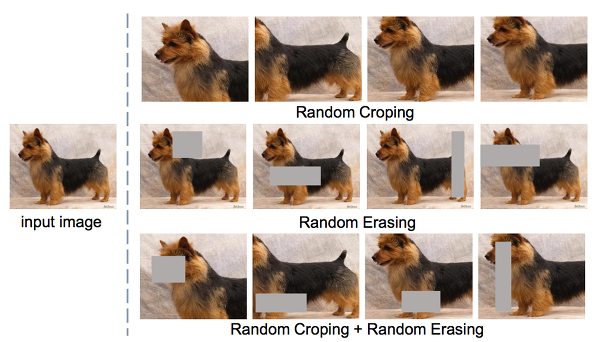
\includegraphics[width=0.6\textwidth]{img/data_augmentation.png}
        \caption{Verschiedene Methoden und Kombinationen zur Datenaugementation.}
        \label{fig:data_augmentation}
    \end{figure}
    
    Eine weitere Technik ist das Horizontale Spiegeln (Horizontal Flipping), bei dem die Bilder horizontal gespiegelt werden. Dadurch werden die Daten umgekehrt und das Modell lernt, Objekte aus verschiedenen Blickwinkeln zu erkennen. 
    Diese Technik ist besonders nützlich, wenn die Orientierung der Objekte in den Bildern nicht von Bedeutung ist.    
    Das Hinzufügen von Rauschen (Noise Addition) ist eine weitere Methode der Datenaugmentierung, bei der Rauschen in die Daten eingefügt wird.
    Dies kann helfen, das Modell widerstandsfähiger gegenüber Störungen zu machen und es auf den Umgang mit realen Daten vorzubereiten.    
    Weitere Techniken umfassen das Skalieren, Drehen, Farbveränderungen und das Hinzufügen von Text oder Objekten zu den Bildern. 

    \begin{figure}[!h]
        \centering
        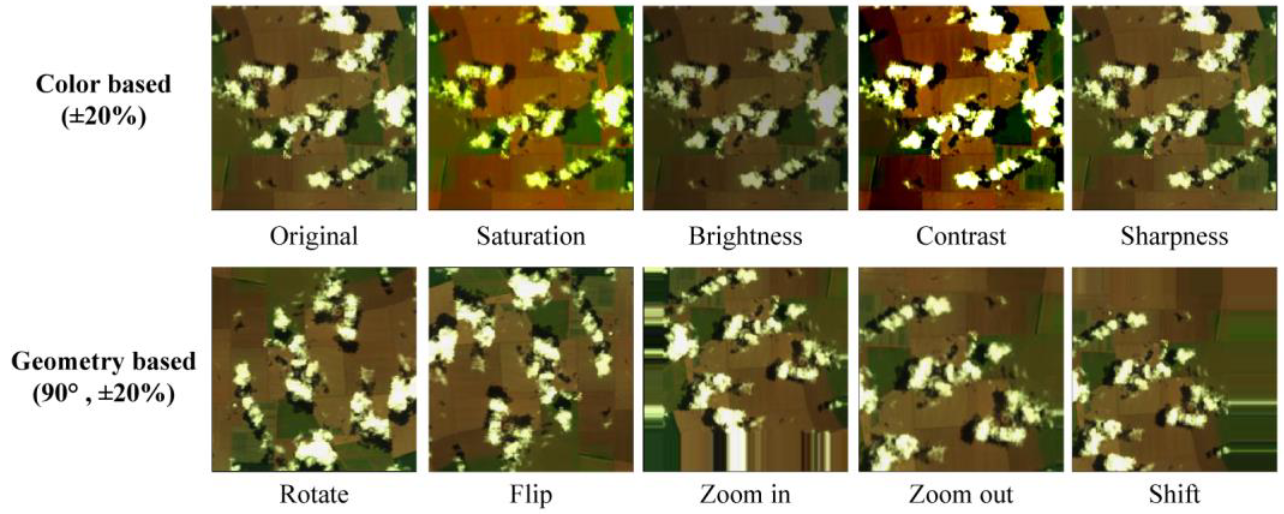
\includegraphics[width=0.6\textwidth]{img/data_augmentation_classics.png}
        \caption{Klassische Methoden und Kombinationen zur Datenaugementation.}
        \label{fig:data_augmentation_classics}
    \end{figure}
    
    Diese Methoden ermöglichen es, den Trainingsdatensatz zu diversifizieren und sicherzustellen, dass das Modell auf verschiedene Situationen und Variationen vorbereitet ist.    
    Insgesamt spielt die Datenaugmentierung eine bedeutende Rolle in der Datenverarbeitung, da sie die Qualität und Vielfalt der Trainingsdaten verbessert. 
    Durch die Anwendung verschiedener Transformationen auf die Daten kann das Modell robustere und leistungsfähigere Modelle erstellen. 
    Es ist wichtig, die richtigen Techniken der Datenaugmentierung entsprechend der Domäne und des Anwendungsfalls auszuwählen, um die Leistung des Modells zu verbessern.
    \footfullcite{shorten2019data,}

\section{Fazit}

Die richtige Vorverarbeitung der Daten ist entscheidend für den Erfolg von Modellen und Analysen. 
Durch Datenbereinigung, Datennormalisierung und Datenaugmentierung kann die Qualität und Aussagekraft der Daten verbessert werden, was zu besseren Ergebnissen führt. 
Die Datenbereinigung ermöglicht es, fehlerhafte oder unvollständige Daten zu entfernen oder zu korrigieren, um eine solide Grundlage für präzise und verlässliche Analysen und Modelle zu schaffen.

Obwohl in diesem Projekt der verwendete Datensatz bereits vorbereitet ist, ist es dennoch wichtig, zu prüfen, ob solch einer den Anforderungen des spezifischen Problems gerecht wird.
Dies könnte die Überlegung beinhalten, ob ein vorgefertigter Datensatz verwendet werden kann oder ob Anpassungen erforderlich sind, um sicherzustellen, dass die Daten die relevanten Informationen für die Analysen enthalten.
    


\chapter{Architektur des DeepLabV3+ Modells mit ResNet-50 Backbone}

Das DeepLabV3+ Modell ist eine leistungsstarke Architektur für die semantische Segmentierung von Bildern. In diesem Kapitel werden wir uns näher mit der Architektur des Modells befassen, insbesondere mit dem ResNet-50 Backbone.

\section{Backbone-Netzwerk}
    Das Backbone-Netzwerk ist für die Extraktion aussagekräftiger Merkmale aus dem Eingangsbild verantwortlich. In diesem Fall basiert das Backbone-Netzwerk auf der ResNet-50 Architektur. ResNet-50 ist ein tiefes CNN, das in verschiedenen Computer Vision Aufgaben herausragende Leistung erzielt hat. Es besteht aus mehreren Faltungs­schichten, die in verschiedene Stufen gruppiert sind, wobei Residualverbindungen zwischen ihnen verwendet werden, um das Problem des verschwindenden Gradienten zu lösen. Diese Residualverbindungen ermöglichen es dem Netzwerk, effektiver zu lernen, indem sie Gradienten über Verbindungen mit geringerer Tiefe propagieren.

\section{Prediction-Head}
    Der Prediction-Head nimmt die von dem Backbone-Netzwerk extrahierten Merkmale und generiert die endgültigen Vorhersagen. Im DeepLabV3+ Modell verwendet der Prediction-Head atrous (oder dilatierte) Faltungen mit unterschiedlichen Dilationsraten, um mehrskalige Informationen zu erfassen. Dadurch kann das Modell sowohl detaillierte lokale Informationen als auch Kontextinformationen berücksichtigen.
    
    Das ursprüngliche DeepLabV3+ Modell wird auf dem ImageNet-Datensatz vortrainiert, der Millionen von gelabelten Bildern aus Tausenden von Kategorien enthält. Dieses Vortraining hilft dem Modell, generische visuelle Merkmale zu erlernen, die für spezifische Aufgaben feinabgestimmt werden können.
    
    Im bereitgestellten Code wird das vortrainierte DeepLabV3+ Modell mit dem ResNet-50 Backbone geladen. Das bedeutet, dass das Backbone die anfänglichen Schichten von ResNet-50 umfasst, die für die Merkmalsextraktion verantwortlich sind. Die genauen Schichten und ihre Konfigurationen können recht komplex sein, aber sie beinhalten in der Regel mehrere Faltungsschichten, Pooling-Schichten zur Verkleinerung der Auflösung und Residualverbindungen.
    
    Die Modifikation im Code betrifft die letzte Schicht des Modells, den Klassifizierer. Im ursprünglichen DeepLabV3+ Modell handelt es sich dabei um eine 1x1-Faltungsschicht, die einen Tensor mit den Dimensionen [Batchgröße, Anzahl der Klassen, Höhe, Breite] erzeugt. Die Anzahl der Klassen im Originalmodell beträgt 21, da es auf dem COCO-Datensatz trainiert wurde, der Objekte aus 21 verschiedenen Kategorien enthält.
    
    Im bereitgestellten Code wird die letzte Schicht jedoch durch eine andere 1x1-Faltungsschicht mit einer geänderten Anzahl von Ausgabekanälen ersetzt. Die ursprüngliche Anzahl von Ausgabekanälen beträgt 256, was der Anzahl der vom Backbone-Netzwerk erlernten Merkmale entspricht. In der modifizierten Version des Codes wird jedoch die Anzahl der Ausgabekanäle auf 3 gesetzt, was darauf hinweist, dass das Modell einen Tensor mit den Dimensionen [Batchgröße, 3, Höhe, Breite] ausgibt. Diese Änderung der Anzahl der Ausgabekanäle erfolgt, um das Modell für eine spezifische Aufgabe mit drei Klassen anstelle der ursprünglichen 21 Klassen anzupassen.
    
    Insgesamt handelt es sich bei dem DeepLabV3+ Modell mit ResNet-50 Backbone um eine leistungsstarke Architektur für semantische Segmentierungsaufgaben. Durch die Modifikation der letzten Schicht passt der Code das Modell an, um Pixel in eine von drei Klassen zu klassifizieren.
    
    \textbf{Code-Beispiel:}
    
    \begin{lstlisting}[language=Python]
    Net = torchvision.models.segmentation.deeplabv3_resnet50(pretrained=True)  # Modell laden
    Net.classifier[4] = torch.nn.Conv2d(
        256,
        3,
        kernel_size=(1, 1),
        stride=(1, 1)
    )  # Letzte Schicht auf 3 Klassen ändern
    Net = Net.to(device)
    
    optimizer = torch.optim.Adam(params=Net.parameters(), lr=Learning_Rate)  # Adam-Optimizer erstellen
    \end{lstlisting}
    
\section{Laden des Modells}
    Der Code beginnt damit, das DeepLabV3+ Modell mit ResNet-50 Backbone mithilfe der torchvision-Bibliothek zu laden. DeepLabV3+ ist ein beliebtes Modell für die semantische Segmentierung, d.h., es weist jedem Pixel in einem Eingangsbild eine Klassenbezeichnung zu. Das ResNet-50 Backbone ist ein Typ von Faltungsneuronalem Netzwerk (CNN), das für seine Effektivität bei der Extraktion von Merkmalen aus Bildern bekannt ist.
    
\section{Modifikation der letzten Schicht}
    Anschließend wird die letzte Schicht des geladenen Modells modifiziert. Im Originalmodell ist die letzte Schicht ein Klassifizierer, der eine Wahrscheinlichkeitsverteilung über 21 verschiedene Klassen (wie "Person", "Auto", "Hund", usw.) erzeugt. In diesem Code wird die letzte Schicht jedoch durch eine 1x1-Faltungsschicht ersetzt. Diese Modifikation ändert die Ausgabe des Modells so, dass eine Wahrscheinlichkeitsverteilung über 3 Klassen anstelle von 21 erzeugt wird. Die spezifischen Werte für die Kernelgröße und den Stride bestimmen das Verhalten der Faltung.

\section{Verschieben des Modells auf ein Gerät}
    Das modifizierte Modell wird dann auf ein spezifiziertes Gerät verschoben, das entweder die CPU oder eine GPU sein kann. Dieser Schritt stellt sicher, dass die Berechnungen, die das Modell durchführt, auf dem ausgewählten Gerät durchgeführt werden. Die Nutzung einer GPU kann die Schulung und Inferenz von Deep Learning Modellen erheblich beschleunigen.

\section{Erstellen des Optimierers}
    Ein Optimierer ist ein Algorithmus, der die Parameter des Modells während des Trainingsprozesses anpasst, um die Verlustfunktion zu minimieren. In diesem Code wird ein Adam-Optimierer erstellt, der das Modellparameter (erhalten durch \texttt{Net.parameters()}) und die Lernrate (angegeben durch \texttt{Learning\_Rate}) als Eingabe verwendet. Die Lernrate bestimmt die Schrittgröße, mit der der Optimierer die Modellparameter basierend auf den berechneten Gradienten während der Rückwärtspropagation aktualisiert.
    
    Indem Sie dieser Architektur folgen, haben Sie ein modifiziertes DeepLabV3+ Modell mit ResNet-50 Backbone, das Bilder in eine von drei Klassen segmentieren kann. Die Modellparameter werden während des Trainings mit dem Adam-Optimierer und der angegebenen Lernrate optimiert.



\chapter{Convolutional Neural Network Trainings Prozess}

\section{Was ist Training?}
    Bevor wir uns mit dem Trainingsprozess von Convolutional Neural Networks (CNNs) befassen, ist es sinnvoll, das Konzept des Trainings von neuronalen Netzwerken kurz aufzufrischen. Training bezieht sich auf den Prozess des Anpassens der Gewichte und Bias-Werte eines neuronalen Netzwerks, um eine bestimmte Aufgabe zu erlernen. Im Fall von CNNs besteht das Ziel darin, das Netzwerk auf eine bestimmte Bildklassifizierung oder ein anderes visuelles Erkennungsproblem vorzubereiten.
    
    Der Trainingsprozess ist von entscheidender Bedeutung für die Leistungsfähigkeit von CNNs. Während des Trainings lernt das Netzwerk, relevante Merkmale aus den Trainingsdaten zu extrahieren und Muster zu erkennen. Durch die Optimierung der Gewichte und Bias-Werte kann das Netzwerk lernen, geeignete Entscheidungen zu treffen und präzise Vorhersagen zu treffen.

\section{Trainingsprozess}
    Der Trainingsprozess eines CNNs lässt sich grob in verschiedene Schritte und Phasen unterteilen. Zunächst werden die Trainingsdaten geladen und gegebenenfalls vorverarbeitet, um eine optimale Eingabe für das Netzwerk zu gewährleisten. Dies kann Aufgaben wie das Skalieren der Bilder, das Normalisieren der Daten oder das Anwenden von Data Augmentation-Techniken umfassen.
    Während des Trainingsprozesses werden die Eingabedaten durch das CNN propagiert, wobei die Convolutional-Schichten und Pooling-Schichten verwendet werden, um Merkmale auf verschiedenen Abstraktionsebenen zu extrahieren. Aktivierungsfunktionen wie die ReLU-Funktion werden angewendet, um die Nichtlinearität des Netzwerks zu erhöhen.
    
    Ein entscheidender Schritt ist die Berechnung des Verlusts (Loss), der den Unterschied zwischen den vom Netzwerk vorhergesagten Ausgaben und den tatsächlichen Labels misst. Die Wahl des geeigneten Verlustmaßes hängt von der spezifischen Aufgabe ab, beispielsweise der Kreuzentropie-Verlust für Klassifizierungsaufgaben.
    Um den Verlust zu minimieren und die Gewichte anzupassen, wird der Backpropagation-Algorithmus angewendet. Dabei werden die Gradienten der Verlustfunktion bezüglich der Gewichte berechnet und anschließend mittels eines Optimierungsverfahrens, wie zum Beispiel dem Stochastic Gradient Descent (SGD), verwendet, um die Gewichte in die richtige Richtung zu aktualisieren.
    
    Der Trainingsprozess wird in der Regel über mehrere Epochen durchgeführt, wobei jede Epoche eine Durchlauf der gesamten Trainingsdaten umfasst. Dies ermöglicht es dem Netzwerk, schrittweise zu lernen und seine Leistung zu verbessern. Es ist auch üblich, das Netzwerk regelmäßig auf einem separaten Validierungsdatensatz zu testen, um die Überanpassung (Overfitting) zu vermeiden.

\section{Stochastic Gradient Descent (SGD)}
    Der Stochastic Gradient Descent\footfullcite{amari1993backpropagation} (SGD) ist ein Optimierungsverfahren, das eine zentrale Rolle im Trainingsprozess von CNNs spielt. Im Gegensatz zum Gradientenabstiegsverfahren (Gradient Descent), bei dem der Verlust über den gesamten Trainingsdatensatz berechnet wird, verwendet SGD eine zufällige Teilmenge der Daten, um den Gradienten zu approximieren.
    
    Der Einsatz von SGD hat mehrere Vorteile. Erstens ermöglicht er eine schnellere Berechnung des Gradienten, da nur eine Teilmenge der Daten betrachtet wird. Zweitens macht die zufällige Auswahl der Daten das Verfahren robuster gegenüber lokalen Minima, da das Netzwerk unterschiedliche Datenmuster im Verlauf des Trainingsprozesses betrachtet.
    
    \begin{figure}[h]
        \centering
        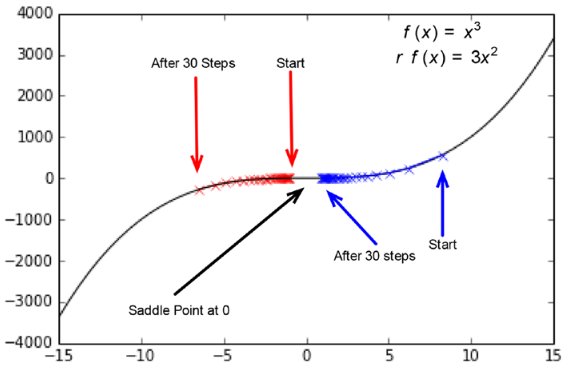
\includegraphics[width=0.8\textwidth]{img/gradient_descent.png}
        \caption{Beispiel von Stochastic Gradient Descent mit 30 Lernschriten.}
        \label{fig:Stochastic_Gradient_Descent}
    \end{figure}
    
    Die Anpassung der Lernrate ist ein wichtiger Aspekt im SGD-Algorithmus. Die Lernrate bestimmt die Größe der Aktualisierungen der Gewichte und beeinflusst somit die Konvergenzgeschwindigkeit des Netzwerks. Eine zu hohe Lernrate kann zu instabilen oder schlecht konvergierenden Lösungen führen, während eine zu niedrige Lernrate den Trainingsprozess verlangsamen kann. Es ist daher oft erforderlich, die Lernrate im Laufe des Trainings anzupassen, beispielsweise durch den Einsatz von Lernrateplanern oder adaptiven Methoden wie Adam.

\section{Backpropagation}
    Backpropagation\footfullcite{amari1993backpropagation} ist ein wesentlicher Bestandteil des Trainingsprozesses von neuronalen Netzwerken, einschließlich CNNs. Es handelt sich um ein Verfahren zur Berechnung der Gradienten der Verlustfunktion bezüglich der Gewichte des Netzwerks.
    
    Der Backpropagation-Algorithmus funktioniert, indem er die Fehlerinformationen vom Ausgabeneuron zurück durch das Netzwerk propagiert. Dabei werden die partiellen Ableitungen der Verlustfunktion nach den Gewichten in den Schichten berechnet. Dies ermöglicht es, den Gradienten des Verlusts bezüglich der Gewichte zu bestimmen und somit die Gewichte entsprechend anzupassen.
    
    Dank der effizienten Berechnung des Backpropagation-Algorithmus ist es möglich, CNNs mit vielen Schichten zu trainieren. Die Gradienten werden schichtweise berechnet, wodurch eine effektive Ausbreitung der Fehler ermöglicht wird. Dieser Prozess des Gradientenabstiegs ermöglicht es dem Netzwerk, seine Gewichte so anzupassen, dass der Verlust minimiert wird.

\section{Hyperparameter-Tuning}
    Hyperparameter\footfullcite{mantovani2016hyper} sind Parameter, die nicht direkt aus den Daten gelernt werden, sondern vor dem Trainingsprozess festgelegt werden müssen. Sie haben einen erheblichen Einfluss auf die Leistungsfähigkeit des CNNs und müssen sorgfältig ausgewählt werden.
    
    Das Tuning von Hyperparametern beinhaltet die Suche nach den besten Werten für diese Parameter, um eine optimale Leistung des CNNs zu erzielen. Dies kann durch manuelles Ausprobieren verschiedener Hyperparameterkombinationen oder durch den Einsatz von automatisierten Methoden wie Grid Search oder Bayesian Optimization erfolgen\footfullcite{amari1993backpropagation}.
    
    \begin{figure}[h]
        \centering
        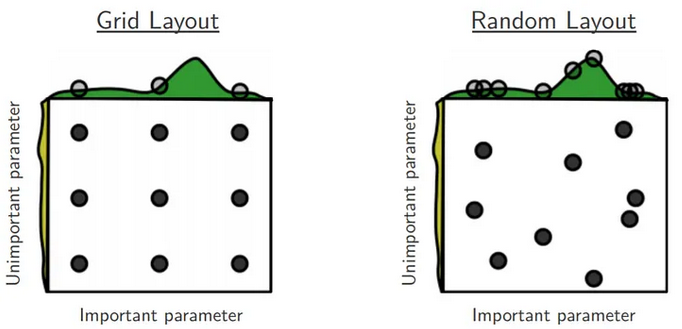
\includegraphics[width=\textwidth]{img/hyperparameter_tuning.png}
        \caption{Hyperparameter tuning.}
        \label{fig:hyperparameter_tuning}
    \end{figure}
    
    Beispiele für Hyperparameter sind die Lernrate, die Anzahl der Schichten und Filter im Netzwerk, die Größe des Mini-Batches, die Dropout-Rate und die Regularisierungsparameter. Das richtige Tuning dieser Hyperparameter kann dazu beitragen, eine bessere Generalisierungsfähigkeit des Netzwerks zu erreichen und Überanpassung zu vermeiden.

\section{Regularisierungstechniken}
    Regularisierungstechniken\footfullcite{ghiasi2018dropblock} sind Methoden, die während des Trainingsprozesses angewendet werden, um die Überanpassung des Netzwerks an die Trainingsdaten zu reduzieren und die allgemeine Leistungsfähigkeit zu verbessern.
    
    Eine gängige Regularisierungstechnik ist die L1- und L2-Regularisierung\footfullcite{ibrahim2023anomaly}, bei der ein Regularisierungsterm zur Verlustfunktion hinzugefügt wird, der die Gewichte des Netzwerks beeinflusst. Dies hilft, die Gewichte zu reduzieren und die Modellkomplexität zu verringern.
    
    Ein weiteres Regularisierungsverfahren ist Dropout\footfullcite{labach2019survey}, bei dem während des Trainings zufällig einige Neuronen deaktiviert werden. Dadurch wird das Netzwerk gezwungen, redundante Merkmale zu lernen und erhöht die Robustheit gegenüber Überanpassung.
    
    Data Augmentation ist eine weitere Regularisierungstechnik, bei der die Trainingsdaten künstlich erweitert werden, indem sie transformiert oder mit Rauschen versehen werden. Dies ermöglicht es dem Netzwerk, mehr Variationen der Daten zu sehen und generalisierbarere Merkmale zu lernen.
    
    Die Anwendung von Regularisierungstechniken während des Trainingsprozesses trägt dazu bei, die Leistungsfähigkeit des CNNs zu verbessern und die Überanpassung an die Trainingsdaten zu reduzieren.

\chapter{Transfer Learning}

\section{Einführung in Transfer Learning}

    Transfer Learning ist eine leistungsstarke Technik im Bereich des Deep Learnings, die es uns ermöglicht, das Wissen von vorgefertigten Modellen zu nutzen und es auf neue Aufgaben anzuwenden.
    Dabei werden die erlernten Repräsentationen oder Parameter eines Modells wiederverwendet und auf eine andere verwandte Aufgabe übertragen. 
    Diese Herangehensweise hat in den letzten Jahren aufgrund ihrer Fähigkeit, Zeit und Rechenressourcen zu sparen und dennoch hohe Leistung bei neuen Aufgaben zu erzielen, erhebliche Aufmerksamkeit und Beliebtheit erlangt.
    Die grundlegende Idee hinter Transfer Learning ist, dass Modelle, die auf großen und vielfältigen Datensätzen wie ImageNet trainiert wurden, allgemeine Merkmale gelernt haben, die für eine Vielzahl von visuellen Erkennungsaufgaben nützlich sind. 
    Anstatt den Lernprozess für eine neue Aufgabe mit begrenzten Daten von Grund auf zu beginnen, können wir unser Modell mit den vorab trainierten Gewichten aus einer verwandten Aufgabe initialisieren. 
    Dadurch besitzt das Modell bereits Wissen über niedrig eingestufte Merkmale, Formen und Muster, was in der neuen Aufgabe von Vorteil sein kann.
    Einer der Hauptvorteile von Transfer Learning besteht darin, das Problem des Datenmangels zu umgehen. 
    Das Sammeln und Markieren großer Datenmengen für jede spezifische Aufgabe kann zeitaufwändig und kostspielig sein. 
    Durch die Nutzung von Transfer Learning können wir jedoch auf die große Menge an markierten Daten zurückgreifen, die für das Vortraining verfügbar sind, und somit den Bedarf an einem großen markierten Datensatz für die Ziel-Aufgabe verringern. 
    Dies ist besonders vorteilhaft in Bereichen, in denen das Erlangen von markierten Daten herausfordernd oder nicht praktikabel ist.
    Ein weiterer Vorteil von Transfer Learning liegt in seiner Fähigkeit zur Generalisierung auf neuen Aufgaben. 
    Indem wir Wissen von vortrainierten Modellen übertragen, nutzen wir effektiv die erlernten Repräsentationen, die aussagekräftige Merkmale erfassen. 
    Diese Fähigkeit zur Generalisierung ermöglicht es dem Modell, auch mit begrenzten Trainingsdaten für die Ziel-Aufgabe gute Leistungen zu erbringen. 
    Es trägt auch zur Reduzierung von Overfitting bei, da das Modell bereits aus einem vielfältigen Datensatz gelernt hat und robuste und diskriminierende Merkmale entwickelt hat.
    Darüber hinaus ermöglicht Transfer Learning, von der Expertise und den Forschungsanstrengungen zu profitieren, die in die Entwicklung vortrainierter Modelle investiert wurden. 
    Viele fortschrittliche Modelle und Architekturen wurden auf groß angelegten Datensätzen vortrainiert und erreichen hohe Genauigkeit bei verschiedenen Benchmark-Aufgaben. 
    Indem man diese vortrainierten Modelle als Ausgangspunkt nutzen, kann man ihre Architekturen und Merkmalsextraktoren verwenden und sie für eine spezifische Aufgabe abstimmen. Dadurch kann der Lernprozess beschleunigt werden.
    \footfullcite{pan2010transfer,yosinski2014transfer}

\section{Pre-Trained Models}

    Ein wichtiger Bestandteil des Transfer Learnings sind vortrainierte Modelle. 
    Diese vortrainierten Modelle sind neuronale Netzwerkmodelle, die auf großen Datensätzen trainiert wurden, in der Regel für eine andere Aufgabe als die aktuelle. 
    Durch das Training auf umfangreichen Datensätzen haben diese Modelle allgemeine Merkmale und Muster erlernt, die für eine Vielzahl von verwandten Aufgaben nützlich sein können.
    Vortrainierte Modelle sind das Ergebnis umfangreicher Trainingsverfahren auf großen Rechenressourcen, um komplexe Muster in den Daten zu erkennen. 
    Typischerweise werden vortrainierte Modelle auf großen Bilderkennungsdatensätzen wie ImageNet trainiert, die Millionen von Bildern mit verschiedenen Klassen umfassen. 
    Während des Trainings lernen diese Modelle, verschiedene visuelle Merkmale wie Kanten, Formen, Texturen und Objekte zu erkennen und zu extrahieren. 
    Durch diese umfangreiche Vorarbeit können vortrainierte Modelle als Ausgangspunkt für andere Aufgaben dienen, indem sie bereits gelernte Merkmale zur Verfügung stellen.
    Die Idee hinter der Verwendung vortrainierter Modelle im Transfer Learning besteht darin, das Wissen und die Merkmale, die in den vortrainierten Modellen enthalten sind, auf neue Aufgaben zu übertragen. 
    Anstatt ein Modell von Grund auf neu zu trainieren, können wir ein vortrainiertes Modell verwenden und es an die spezifischen Anforderungen unserer Aufgabe anpassen. 
    Da vortrainierte Modelle bereits eine gewisse Vorstellung von visuellen Merkmalen haben, können sie uns dabei unterstützen, auch mit begrenzten Daten gute Ergebnisse zu erzielen.
    Bei der Verwendung vortrainierter Modelle müssen wir jedoch beachten, dass die vortrainierte Aufgabe und die aktuelle Aufgabe zusammenpassen sollten.
    Wenn die vortrainierte Aufgabe ähnliche Merkmale oder Konzepte wie die aktuelle Aufgabe beinhaltet, ist die Wahrscheinlichkeit höher, dass das Transfer Learning erfolgreich ist. 
    Zum Beispiel könnte ein vortrainiertes Modell, das auf Bilderkennung trainiert wurde, als Ausgangspunkt für eine Aufgabe der Objekterkennung dienen, da beide Aufgaben visuelle Merkmale nutzen.

\section{Fine-tuning von vortrainierten Modellen}

    Die Feinabstimmung (Fine-tuning) ist ein wichtiger Schritt im Transfer Learning, der es ermöglicht, ein vortrainiertes Modell für eine spezifische Aufgabe anzupassen. 
    Bei der Feinabstimmung wird das vortrainierte Modell zunächst als Ausgangspunkt verwendet und anschließend werden die Gewichte des Modells mithilfe eines kleineren, auf die spezifische Aufgabe zugeschnittenen Datensatzes aktualisiert. 
    Dieser Prozess erlaubt es dem Modell, sich an die spezifischen Merkmale und Nuancen der neuen Aufgabe anzupassen.
    Der erste Schritt bei der Feinabstimmung besteht darin, das vortrainierte Modell zu laden, das auf einer großen, allgemeinen Aufgabe trainiert wurde. Dieses Modell verfügt bereits über ein gewisses Verständnis von visuellen Merkmalen, das durch das Training auf umfangreichen Datensätzen erworben wurde. 
    Anschließend werden die oberen Schichten des Modells, die für die spezifische Aufgabe weniger relevant sind, eingefroren, um zu verhindern, dass sie während des Trainings aktualisiert werden. 
    Dies ermöglicht es uns, die vortrainierten Merkmale beizubehalten, während wir die Gewichte der unteren Schichten des Modells anpassen.
    Der nächste Schritt besteht darin, ein kleineres, auf die spezifische Aufgabe zugeschnittenes Datenset zu verwenden, um das Modell zu trainieren. 
    Da die Anzahl der verfügbaren Daten möglicherweise begrenzt ist, ist es wichtig, Overfitting zu vermeiden und gleichzeitig das Modell an die spezifischen Merkmale der neuen Aufgabe anzupassen. 
    Durch die Verwendung eines kleineren Datensatzes können wir die Rechenressourcen effizienter nutzen und den Trainingsprozess beschleunigen.
    Während des Trainingsprozesses werden die Gewichte der unteren Schichten des Modells aktualisiert, um die Merkmale der neuen Aufgabe besser zu erfassen. 
    Da die oberen Schichten des Modells eingefroren sind, bleiben die bereits erlernten Merkmale erhalten, während die Gewichte der unteren Schichten an die neuen Daten angepasst werden. 
    Dadurch kann das Modell spezifische Muster und Merkmale der neuen Aufgabe erlernen, während es gleichzeitig von den allgemeinen Merkmalen des vortrainierten Modells profitiert.
    Die Feinabstimmung bietet mehrere Vorteile. 
    Erstens ermöglicht sie eine schnellere Konvergenz, da das Modell bereits über eine gute initiale Gewichtung verfügt und somit weniger Trainingsiterationen benötigt werden. 
    Zweitens kann die Leistung des Modells durch die Anpassung an die spezifischen Merkmale der neuen Aufgabe verbessert werden.
    Indem das Modell auf die Besonderheiten der neuen Aufgabe abgestimmt wird, kann es genauere Vorhersagen treffen und bessere Ergebnisse erzielen.

\section{Verwendung von vortrainierten Modellen}

    Eine alternative Methode des Transfer Learning besteht darin, das vortrainierte Modell als festen Merkmalsextraktor zu verwenden. 
    Dabei werden die Faltungsschichten des vortrainierten Modells genutzt, um Merkmale aus den Eingabedaten zu extrahieren, die anschließend einem neuen Klassifikator oder Regressor zugeführt werden. 
    Dieser Ansatz bietet verschiedene Vorteile, wie zum Beispiel die Möglichkeit, vortrainierte Modelle auf kleineren Datensätzen einzusetzen.
    Bei dieser Methode werden die Gewichte des vortrainierten Modells beibehalten und die oberen Schichten eingefroren, um sicherzustellen, dass die bereits erlernten Merkmale nicht verändert werden. 
    Die Faltungsschichten des Modells dienen dann als Merkmalsextraktoren, die relevante Informationen aus den Eingabedaten extrahieren. 
    Diese Merkmale werden anschließend als Eingabe für einen neuen Klassifikator oder Regressor verwendet, der auf die spezifische Aufgabe abgestimmt ist.
    Der Vorteil dieser Vorgehensweise liegt darin, dass das vortrainierte Modell bereits über ein umfangreiches Wissen verfügt, das auf großen Datensätzen trainiert wurde. 
    Indem wir diese vortrainierten Merkmalsextraktoren verwenden, können wir von dem bereits erlernten Wissen profitieren, ohne das gesamte Modell neu trainieren zu müssen. 
    Dies ist insbesondere dann vorteilhaft, wenn wir nur über einen begrenzten Datensatz verfügen, da das Training eines Modells von Grund auf mit wenigen Daten schwierig sein kann.
    Ein weiterer Vorteil besteht darin, dass die Merkmalsextraktionsschichten des vortrainierten Modells bereits gute Ergebnisse bei der Erkennung allgemeiner Merkmale erzielen. 
    Dies ermöglicht es uns, auch auf kleineren Datensätzen aussagekräftige Merkmale zu extrahieren und sie als Eingabe für den Klassifikator oder Regressor zu verwenden. 
    Somit können wir die Vorteile des vortrainierten Modells nutzen, um bessere Ergebnisse auf unseren spezifischen Aufgaben zu erzielen.
    Es ist wichtig zu beachten, dass die Verwendung vortrainierter Modelle als Merkmalsextraktoren bestimmte Einschränkungen hat. 
    Da die oberen Schichten des Modells eingefroren sind, können sie nicht auf die spezifischen Merkmale der neuen Aufgabe angepasst werden. 
    Daher ist diese Methode besonders geeignet, wenn die Merkmale der neuen Aufgabe bereits in den vortrainierten Schichten erfasst werden können. 
    In solchen Fällen bietet die Nutzung der vortrainierten Merkmalsextraktoren eine effiziente Möglichkeit, um genaue Vorhersagen zu treffen.

\section{Anwendung von DeepLabV3 ResNet50}

    In diesem Abschnitt wird die konkrete Umsetzung des Transfer Learning in unserem Projekt durch die Verwendung des DeepLabV3 ResNet50-Modells erläutert.
    DeepLabV3 ist eine hochmoderne Architektur, die für semantische Segmentierungsaufgaben entwickelt wurde und für ihre herausragende Leistung in der Bildverarbeitung und Szenenanalyse bekannt ist.
    Das ResNet50 dient als grundlegende Netzwerkstruktur innerhalb des DeepLabV3-Frameworks und nutzt Residual-Lernen, um das Training tiefer faltungs­basierter neuronaler Netzwerke zu erleichtern.
    Die Entscheidung, das DeepLabV3 ResNet50-Modell in unserem Projekt zu verwenden, basierte auf einer Vielzahl von Überlegungen.
    Die Architektur des Modells hat sich insbesondere im Bereich der semantischen Segmentierung als äußerst leistungsstark erwiesen, was eine wesentliche Aufgabe in unseren Projektzielen darstellt.
    Durch den Einsatz des DeepLabV3 ResNet50-Modells kann man das umfangreiche Training und die erlernten Repräsentationen nutzen, die das Modell auf großen Datensätzen erfasst hat.
    Dadurch kann das Netzwerk feine semantische Details in unserem spezifischen Anwendungsbereich erkennen.
    Die Verwendung eines vortrainierten Modells wie DeepLabV3 ResNet50 bietet eine Vielzahl von Vorteilen.
    Ein bemerkenswerter Vorteil besteht darin, dass man das Wissen, das durch vorherige Modelle erlangt wurde, in das Projekt übertragen kann, ohne ein neuronales Netzwerk von Grund auf trainieren zu müssen.
    Das vortrainierte Modell enthält eine Vielzahl von allgemeinen Merkmalen und Mustern, die während der umfangreichen Exposition des Modells gegenüber vielfältigen visuellen Daten während seiner Trainingsphase erlernt wurden.
    Durch die Nutzung dieser erlernten Merkmale kann man die Entwicklungsdauer des Projekts verkürzen und die Rechenbelastung, die mit dem Training eines Modells von Grund auf verbunden ist, verringern.
    Darüber hinaus bietet das DeepLabV3 ResNet50-Modell eine solide Grundlage für die Feinabstimmung, die es ermöglicht, das Netzwerk an spezifische Aufgaben anzupassen.
    Bei der Feinabstimmung werden die vortrainierten Gewichte des Netzwerks beibehalten und an die Feinheiten des Ziel-Datensatzes angepasst.
    Dieser Prozess ermöglicht eine schnellere Konvergenz des Lernprozesses des Modells, verkürzt die Gesamttrainingszeit und verbessert die endgültige Leistung bei der Segmentierungsaufgabe.
    Die Feinabstimmung ermöglicht es auch, das im vortrainierten Modell vorhandene Wissen an die spezifische Anwendungsdomäne anzupassen.
    Dabei können die allgemeinen Merkmale, die vom Modell extrahiert wurden, verfeinert und an die Feinheiten der Zielaufgabe angepasst werden.
    Zusammenfassend bietet die Einbindung des DeepLabV3 ResNet50-Modells in das Projekt mittels Transfer Learning eine solide Grundlage, um eine präzise semantische Segmentierung zu erreichen. 
    Indem man auf das vorhandene Wissen des Modells zurückgreift und die Vorteile der Feinabstimmung nutzt, kann man die Fachkenntnisse von DeepLabV3 ResNet50 nutzen und sie effektiv auf die einzigartige Anwendungsdomäne anpassen. 
    Diese Vorgehensweise beschleunigt nicht nur den Entwicklungsprozess des Projekts, sondern führt auch zu einer hochwertigen Lösung, indem das Modell von seinem umfangreichen Training mit vielfältigen visuellen Daten profitiert.
    Ein entscheidender Aspekt bei der Anwendung des DeepLabV3 ResNet50-Modells besteht darin, dass die vortrainierten Gewichte des Modells eingefroren bleiben, um die extrahierten Merkmale beizubehalten. 
    Die Faltungsschichten des Modells werden verwendet, um Merkmale aus den Eingabedaten zu extrahieren, die dann in einen neuen Klassifizierer oder Regressor eingespeist werden können. 
    Dieser Ansatz ermöglicht es, die Vorteile des vortrainierten Modells als leistungsstarken Feature-Extraktor zu nutzen, während man gleichzeitig einen neuen, auf die spezifische Aufgabe abgestimmten Klassifizierer oder Regressor trainiert.
    Die Verwendung von vortrainierten Modellen als Feature-Extraktoren bietet eine Reihe von Vorteilen. Insbesondere kann man auf kleineren Datensätzen arbeiten, da die vortrainierten Modelle bereits allgemeine Merkmale gelernt haben, die auf verschiedene Aufgaben übertragbar sind. 
    Dadurch wird der Bedarf an großen Trainingsdatensätzen reduziert, was sowohl die Datenbeschaffung als auch die Rechenressourcen erleichtert. 
    Darüber hinaus ermöglicht die Verwendung von vortrainierten Modellen als Feature-Extraktoren eine schnellere Entwicklung von Modellen, da der Schwerpunkt auf der Anpassung des Klassifizierers oder Regressors liegt, anstatt das gesamte Modell von Grund auf neu zu trainieren.
    Insgesamt bietet die Anwendung des DeepLabV3 ResNet50-Modells als Feature-Extraktor eine effektive Methode des Transfer Learning, um hochwertige Ergebnisse in der semantischen Segmentierungsaufgabe zu erzielen. 
    Durch die Kombination der Stärken des vortrainierten Modells und der Anpassung an die spezifische Anwendungsdomäne kann man die Effizienz verbessern und gleichzeitig genaue und zuverlässige Ergebnisse erzielen.


\chapter{Common Challenges and Solutions}

\section{Overfitting and underfitting}
\section{Vanishing and exploding gradients}
\section{Gradient descent optimization}
\section{Solutions to common challenges}


% Ist nur als platzhalter gedacht..

\chapter{Tools and Frameworks for CNN Training}

\section{PyTorch}
Introduce PyTorch as a popular deep learning framework known for its flexibility and dynamic computational graph. Discuss its key features, such as automatic differentiation, GPU acceleration, and extensive support for neural network architectures. Provide examples of PyTorch code snippets to demonstrate its ease of use and showcase its capabilities for CNN training.

\section{TensorFlow}
Discuss TensorFlow, one of the most widely used deep learning frameworks. Explain its static computational graph paradigm and its ability to efficiently utilize GPUs for accelerated training. Discuss TensorFlow's ecosystem, which includes high-level APIs like Keras and TensorFlow 2.0's eager execution mode. Illustrate the usage of TensorFlow through code snippets and highlight its strengths and popularity in the deep learning community.

\section{Keras}
Introduce Keras as a high-level deep learning library that runs on top of TensorFlow, CNTK, or Theano. Emphasize Keras' user-friendly interface, which simplifies the process of building, training, and evaluating neural networks. Discuss its versatility in supporting various neural network architectures, including CNNs, and its integration with popular backends. Provide examples of Keras code snippets to showcase its simplicity and accessibility.

\section{Caffe}
Discuss Caffe, a deep learning framework widely used for its efficiency and speed in CNN training. Explain Caffe's model definition language, which allows easy specification of network architectures. Discuss Caffe's pre-trained models and model zoo, which provide a vast collection of well-performing models for various tasks. Describe its popularity in computer vision applications and provide examples of Caffe code snippets.

\section{Other Popular Frameworks}
Discuss other notable deep learning frameworks that are commonly used for CNN training. Include frameworks such as MXNet, Theano, and Torch. Highlight their unique features, advantages, and any notable use cases. Briefly explain how they compare to the previously discussed frameworks.

\chapter{Schlusswort}

\section{Zusammenfassung und Fazit der Arbeit}

Das Ziel dieser Arbeit war es, einen umfassenden Überblick über Skalierungsmethoden in der Bildverarbeitung zu geben.
In den Grundlagen wurden verschiedene Arten der Skalierung und wichtige Aspekte behandelt. Anschließend wurden klassische Skalierungsmethoden wie Pixel-Verdopplung, Nearest-Neighbor-Interpolation, bilineare Interpolation, Bikubische Interpolation und Lanczos-Interpolation untersucht und deren Vor- und Nachteile analysiert.

Darüber hinaus wurden fortgeschrittene Skalierungsmethoden wie Convolutional Neural Networks (CNNs), Super Resolution, Generative Adversarial Networks (GANs) und Multiscale-Skalierung vorgestellt.
Es wurde auf die Grundlagen, Architekturen, Anwendungen und Limitationen dieser Methoden eingegangen.

Die Evaluation von Skalierungsmethoden wurde anhand verschiedener Qualitätsmetriken wie Peak Signal-to-Noise Ratio (PSNR), Structural Similarity Index Measure (SSIM) und Mean Opinion Score (MOS) durchgeführt.
Zudem wurden Kriterien zur Auswahl der geeigneten Skalierungsmethode diskutiert.

Ein Schwerpunkt der Arbeit lag auf der Einführung in Deep Learning und speziell Convolutional Neural Networks.
Die Architektur von CNNs, deren Anwendungen und der Trainingsprozess wurden detailliert erläutert.
Des Weiteren wurde die Bedeutung von Datenverarbeitung, einschließlich Datennormalisierung und Datenaugmentierung, betont.

Abschließend wurden gängige Herausforderungen und Lösungen im Bereich des Deep Learning diskutiert, wie Overfitting, Exploding und Vanishing Gradients sowie Gradient Descent Optimization.
Verschiedene Tools und Frameworks für das Training von CNNs, wie PyTorch, TensorFlow, Keras und Caffe, wurden vorgestellt.

Zusammenfassend liefert diese Arbeit einen umfassenden Einblick in Skalierungsmethoden und deren Anwendungen in der Bildverarbeitung.
Zukünftige Forschungsrichtungen könnten sich auf die Verbesserung der Skalierungsgenauigkeit, die Effizienz der Methoden und die Anwendung auf spezifische Domänen konzentrieren.

\section{Perspektiven für zukünftige Forschungen}

In Anbetracht der vorliegenden Forschungsergebnisse und des implementierten Bildverarbeitungsverfahrens zur Segmentierung und Auswertung von Füllständen in Bildern eröffnen sich mehrere vielversprechende Perspektiven für zukünftige Forschungen. Diese Perspektiven können zur weiteren Verbesserung der Bildverarbeitungsmethoden und neuronalen Netze sowie zur Erweiterung des Anwendungsbereichs beitragen. Im Folgenden werden einige relevante Themen für zukünftige Forschungen skizziert:

\subsection{Optimierung der Bildverarbeitungsmethoden}

Obwohl die in dieser Studienarbeit verwendeten Bildverarbeitungsmethoden gute Ergebnisse bei der Füllstandserkennung gezeigt haben, gibt es noch Raum für Verbesserungen. Zukünftige Forschungen könnten darauf abzielen, neue Bildverarbeitungstechniken zu entwickeln oder vorhandene Methoden weiter zu optimieren, um die Genauigkeit und Effizienz der Füllstandserkennung zu steigern. Die Verwendung fortschrittlicher Algorithmen zur Bildverbesserung, Rauschunterdrückung und Kantenextraktion könnte beispielsweise zu präziseren Segmentierungsergebnissen führen. Darüber hinaus könnten adaptive Methoden untersucht werden, die sich an verschiedene Arten von Behältern und Beleuchtungsbedingungen anpassen können.

\subsection{Integration fortschrittlicher neuronaler Netze}

Die vorgestellten neuronalen Netzwerkarchitekturen haben sich als wirksam erwiesen, aber es gibt noch viele weitere Architekturen und Ansätze, die in Betracht gezogen werden könnten. Zukünftige Forschungen könnten den Einsatz fortschrittlicher neuronaler Netze wie Convolutional Neural Networks (CNNs), Recurrent Neural Networks (RNNs) oder Transformer-Netzwerken für die Füllstandserkennung untersuchen. Diese Netze könnten in Kombination mit Transfer Learning oder generativen Modellen wie Generative Adversarial Networks (GANs) eingesetzt werden, um bessere Ergebnisse zu erzielen und die Robustheit gegenüber verschiedenen Szenarien und Datenqualitäten zu verbessern.

\subsection{Erweiterung des Anwendungsbereichs}

Die Anwendung des entwickelten Bildverarbeitungsverfahrens wurde auf die Segmentierung und Auswertung von Füllständen in Bildern beschränkt. Zukünftige Forschungen könnten jedoch den Anwendungsbereich erweitern und das Verfahren auf andere ähnliche Aufgaben anwenden. Beispielsweise könnten ähnliche Techniken zur Erkennung und Klassifizierung von Objekten in Bildern eingesetzt werden, oder das Verfahren könnte auf andere Bildverarbeitungsaufgaben wie Gesichtserkennung, medizinische Bildgebung oder autonome Fahrzeuge angewendet werden. Eine solche Erweiterung würde dazu beitragen, die Einsatzmöglichkeiten des entwickelten Verfahrens zu erweitern und dessen praktischen Nutzen zu maximieren.

\subsection{Evaluation auf größeren und vielfältigeren Datensätzen}

Eine weitere vielversprechende Perspektive für zukünftige Forschungen besteht darin, das entwickelte Bildverarbeitungsverfahren auf größeren und vielfältigeren Datensätzen zu evaluieren. Die in dieser Studienarbeit verwendeten Datensätze waren begrenzt und möglicherweise nicht repräsentativ für alle potenziellen Anwendungsfälle. Zukünftige Forschungen könnten die Performance des Verfahrens auf umfangreicheren Datensätzen mit unterschiedlichen Behältertypen, Füllstandsniveaus und Beleuchtungsbedingungen untersuchen. Dies würde dazu beitragen, die Robustheit und Allgemeingültigkeit des Verfahrens zu validieren und mögliche Einschränkungen oder Herausforderungen bei der Anwendung auf verschiedene Szenarien aufzudecken.

\subsection{Integration von Echtzeitverarbeitung und Echtzeitfeedback}

Die Echtzeitverarbeitung von Bildern und das Echtzeitfeedback sind für viele Anwendungen entscheidend. Zukünftige Forschungen könnten darauf abzielen, das entwickelte Bildverarbeitungsverfahren so zu optimieren, dass es in Echtzeit arbeitet und sofortiges Feedback zu den Füllstandsergebnissen liefert. Dies würde den praktischen Nutzen des Verfahrens erheblich erhöhen und es für Anwendungen in Echtzeitüberwachungssystemen, automatisierten Prozessen oder reaktiven Steuerungssystemen geeignet machen. Die Integration von fortschrittlichen Technologien wie GPUs, FPGAs oder spezialisierten Hardwareplattformen könnte erforscht werden, um die Verarbeitungsgeschwindigkeit zu verbessern und die Latenzzeiten zu minimieren.

\subsection{Integration von KI-gestütztem Lernen}

Die Integration von KI-gestütztem Lernen in das entwickelte Bildverarbeitungsverfahren könnte einen weiteren Forschungsbereich darstellen. Zukünftige Forschungen könnten untersuchen, wie das Verfahren durch die kontinuierliche Analyse und das Lernen aus den erfassten Füllstandsinformationen verbessert werden kann. Die Anwendung von Reinforcement Learning oder Online-Learning-Methoden könnte es dem Verfahren ermöglichen, sich an neue Gegebenheiten, Veränderungen in den Behälterbedingungen oder individuelle Präferenzen anzupassen. Durch die Integration von KI-gestütztem Lernen könnte das Verfahren adaptiver und selbstlernender werden, was zu einer kontinuierlichen Verbesserung der Leistung und der Anpassungsfähigkeit führen würde.

\subsection{Berücksichtigung von Datenschutz und Sicherheit}

Ein wichtiger Aspekt bei der weiteren Erforschung und Anwendung von Bildverarbeitungsmethoden und neuronalen Netzen ist die Berücksichtigung von Datenschutz und Sicherheit. Zukünftige Forschungen sollten den Schutz personenbezogener Daten und die Vermeidung von Missbrauch oder unerwünschter Überwachung in Betracht ziehen. Die Entwicklung von Datenschutzrichtlinien, Anonymisierungstechniken oder Privatsphäreschutzmechanismen könnte erforscht werden, um sicherzustellen, dass das entwickelte Verfahren ethischen Richtlinien und gesetzlichen Bestimmungen entspricht.

\subsection{Integration von weiteren Sensordaten} 

Die Integration von weiteren Sensordaten in die Füllstandserkennung könnte eine interessante Forschungsrichtung sein. Zukünftige Untersuchungen könnten die Möglichkeit erforschen, zusätzliche Sensorinformationen wie Druck-, Temperatur- oder Schwingungssensoren in das Bildverarbeitungsverfahren zu integrieren. Durch die Kombination von Bildinformationen mit anderen Messdaten könnten genauere Füllstandsinformationen gewonnen werden und eine umfassendere Analyse des Behälterzustands ermöglicht werden.

\subsection{Langzeitstudien zur Zuverlässigkeit und Stabilität}

Um die Langzeitzuverlässigkeit und Stabilität des entwickelten Bildverarbeitungsverfahrens zu gewährleisten, könnten zukünftige Forschungen Langzeitstudien durchführen. Durch die kontinuierliche Überwachung und Bewertung der Leistung des Verfahrens über einen längeren Zeitraum hinweg könnten potenzielle Auswirkungen von Umweltbedingungen, Alterungseffekten oder Änderungen in den Einsatzumgebungen ermittelt werden. Dies würde helfen, die praktische Anwendbarkeit des Verfahrens im Langzeitbetrieb zu bewerten und gegebenenfalls Optimierungen oder Wartungsmaßnahmen vorzunehmen.

Insgesamt bieten diese Perspektiven für zukünftige Forschungen spannende Möglichkeiten zur Weiterentwicklung und Verbesserung der Bildverarbeitungsmethoden und neuronalen Netze zur Segmentierung und Auswertung von Füllständen in Bildern. Die vorgeschlagenen Forschungsthemen können zur Weiterentwicklung des Fachgebiets beitragen und den praktischen Nutzen dieser Technologien in verschiedenen Anwendungsdomänen erweitern.

MIIAAUUUUU
ψ(._. )>


\clearpage
%%%%%%%%%%%%%%%%%%%%%%%%%%%%%%%%%%%%%%%%%%%%%%%%%%%%%%%%%%%%%%%%%%%%%%%%%%%%%%
%% Descr:       Vorlage für Berichte der DHBW-Karlsruhe, Datei mit Abkürzungen
%% Author:      Prof. Dr. Jürgen Vollmer, vollmer@dhbw-karlsruhe.de
%% $Id: abk.tex,v 1.4 2017/10/06 14:02:03 vollmer Exp $
%% -*- coding: utf-8 -*-
%%%%%%%%%%%%%%%%%%%%%%%%%%%%%%%%%%%%%%%%%%%%%%%%%%%%%%%%%%%%%%%%%%%%%%%%%%%%%%%

\chapter*{Abkürzungsverzeichnis}                   % chapter*{..} -->   keine Nummer, kein "Kapitel"
						         % Nicht ins Inhaltsverzeichnis
% \addcontentsline{toc}{chapter}{Akürzungsverzeichnis}   % Damit das doch ins Inhaltsverzeichnis kommt

% Hier werden die Abkürzungen definiert
\begin{acronym}[DHBW]
  % \acro{Name}{Darstellung der Abkürzung}{Langform der Abkürzung}
 \acro{Abk}[Abk.]{Abkürzung}

 % Folgendes benutzen, wenn der Plural einer Abk. benöigt wird
 % \newacroplural{Name}{Darstellung der Abkürzung}{Langform der Abkürzung}
 \newacroplural{Abk}[Abk-en]{Abkürzungen}

 \acro{H2O}[\ensuremath{H_2O}]{Di-Hydrogen-Monoxid}

 % Wenn neicht benutzt, erscheint diese Abk. nicht in der Liste
 \acro{NUA}{Not Used Acronym}
\end{acronym}
              % Abkürzungsverzeichnis
\listoffigures             % Liste der Abbildungen
\listoftables              % Liste der Tabellen
\lstlistoflistings         % Liste der Listings
\listofequations           % Liste der Formeln

% Ab hier beginnt der Anhang
\appendix
\addcontentsline{toc}{chapter}{Anhang}

\addcontentsline{toc}{chapter}{Index}
\printindex

\addcontentsline{toc}{chapter}{Literaturverzeichnis}

% Haben Sie das "biblatex"-Paket nicht installiert, benutzen Sie folgendes:
% Ohne das "biblatex"-Paket (s. bericht.sty) produziert folgendes
% "deutsche" Zitate in Literaturverzeichnissen gemaß der Norm DIN 1505,
% Teil 2 vom Jan. 1984.
% Die Zitatmarken werden alphabetisch nach Verfassern
% sortiert und sind durch abgekürzte Verfasserbuchstaben plus
% Erscheinungsjahr in eckigen Klammern gekennzeichnet.

% \bibliographystyle{alphadin}
% \bibliography{bericht}

%%%%%%%%%%%%%%%%%%%%%%%%%%%%%%%%%%%%%%%5
% BIBLATEX
% Benutzt man das "biblatex"-Paket, muß man folgendes schreiben:
\def\refname{Literaturverzeichnis}
\printbibliography
%%%%%%%%%%%%%%%%%%%%%%%%%%%%%%%%%%%%%%%5


%%%%%%%%%%%%%%%%%%%%%%%%%%%%%%%%%%%%%%%%%%%%%%%%%%%%%%%%%%%%%%%%%%%%%%%%%%%%%%%
%% Descr:       Vorlage für Berichte der DHBW-Karlsruhe, Änderungshistorie
%% Author:      Prof. Dr. Jürgen Vollmer, vollmer@dhbw-karlsruhe.de
%% $Id: changelog.tex,v 1.16 2020/03/13 15:12:39 vollmer Exp $
%% -*- coding: utf-8 -*-
%%%%%%%%%%%%%%%%%%%%%%%%%%%%%%%%%%%%%%%%%%%%%%%%%%%%%%%%%%%%%%%%%%%%%%%%%%%%%%%

\chapter*{Änderungen}

\begin{description}
\item[2020/03/13] Tippfehler korrigiert\\
                  aktuelle Formulierungen aus der Prüfungsordnung Technik übernommen\\
                  Formatdatei erklärt
\item[2017/10/06] Anpassung an neuer Versionen diverse Pakete.
\item[2016/03/16] Auf UTF-8 umgestellt, Indices.
\item[2010/04/12] ToDo-Markierungen mit dem \verb+\todo+-Kommando.
\item[2010/01/27] Anhang (\texttt{appendix}), Selbständigkeits-Erklärung, \texttt{framed}-Paket.
\item[2010/01/21] Abkürzungen (\texttt{acronym}), \texttt{table} und \texttt{tabular} benutzt,
     unübliche Pakete beigelegt.
\item[2010/01/18] Code-Listings (\texttt{listings}), Literaturreferenzen \texttt{biblatex})
\item[2010/01/11] Initiale Version.
\end{description}


\newpage
\addcontentsline{toc}{chapter}{Liste der ToDo's}
\listoftodos[Liste der ToDo's]


\end{document}
